% ------------------------------------------------------------
% This is a template for technical reports
% The Main_thesis.txt is the master control file. It is like the
% main function in a C code. Here we use it to load individual chapters.

% Author: Pham Hung Thinh, NTU, Singapore
% Date: 12, 2012
% Template from: Xiao Xiong, NTU, Singapore
% ------------------------------------------------------------


%----------------------------------------------------------------------------
% File          PpHd.tex
% Author        Ong Kok Leong
% Description   preamble: the global settings
%-----------------------------------------------------------------------------

% 1. Define your report format here
\documentclass[12pt,a4paper,twoside]{report}

% 2. Specify the packages to be included
\usepackage{graphicx}
\usepackage{subfigure,amssymb,amsmath,epsfig,fancyheadings,citesort}
\usepackage{times,eqnarray,amsmath,epsfig}
\usepackage{pgfplots}
\pgfplotsset{compat=1.5}
\usepackage{todonotes}
\usepackage{booktabs}

\usepackage{tikz}
\usepackage{xcolor}	
\usepackage{makecell}
\usepackage{slashbox}
\usetikzlibrary{arrows, positioning, calc}

\oddsidemargin  +0.10in %
\evensidemargin +0.00in %
\topmargin      +0.15in %
\textheight     +8.50in %
\textwidth      +6.25in %

\pagestyle{plain}

\font\Bold=cmbx10 scaled \magstep3
\def\EndOfProof{\nolinebreak\ \hfill\rule{1.5mm}{2.7mm}}
\def\endOfProof{\ \hfill\rule{1.5mm}{2.7mm}}

\def\proof{\noindent \textbf{Proof:}\quad}

%\renewcommand{\theequation}{\mbox{\rm Eq.\ \thechapter.\arabic{equation}}}

\newcounter{theorem}
\newtheorem{theorem}{Theorem}
\renewcommand{\thetheorem}{\thechapter.\arabic{theorem}}

\newcounter{lemma}
\newtheorem{lemma}{Lemma}
\renewcommand{\thelemma}{\thechapter.\arabic{lemma}}

\newcounter{corollary}
\newtheorem{corollary}{Corollary}
\renewcommand{\thecorollary}{\thechapter.\arabic{corollary}}

\newcounter{definition}
\newtheorem{definition}{Definition}
\renewcommand{\thedefinition}{\thechapter.\arabic{definition}}

\newcounter{algo}
\newtheorem{algo}{Algorithm}
\renewcommand{\thealgo}{\thechapter.\arabic{algo}}

\renewcommand{\thefigure}{\thechapter.\arabic{figure}}
\renewcommand{\thesubfigure}{\thefigure.\alph{subfigure}}
\makeatletter
\renewcommand{\@thesubfigure}{\thesubfigure:\space}
\renewcommand{\p@subfigure}{}

\def\LEQ.#1.#2.#3{#1\!\leqslant\!#2\!\leqslant\!#3}
\def\GEQ.#1.#2.#3{#1\!\geqslant\!#2\!\geqslant\!#3}
\def\emptyset{\varnothing}
\renewcommand{\theenumi}{\rm \roman{enumi}}
\renewcommand{\labelenumi}{\rm (\theenumi)}
\renewcommand{\theenumii}{\rm \alph{enumii}}
\renewcommand{\labelenumii}{\rm (\theenumii)}

\renewcommand{\topfraction}{0.75}
\renewcommand{\bottomfraction}{0.75}
\renewcommand{\textfraction}{0.10}

%
% Report specific definitions
%

%
% Definition in the context of this report.
%
\def\reporttitle    {An Algorithmic Framework for Web Data Mining}
\def\supp           {\varphi}
\def\psupp          {\varphi^{\mathcal{P}}}
\def\conf           {\delta}
\def\pconf          {\delta^{\mathcal{P}}}
\def\tab            {\hspace{0.8cm}}

%
% Define the set of symbols for the constraint set.
%
\def\map            {\Pi}
\def\gen            {\Upsilon}
\def\prune          {\Phi}
\def\selcand        {\Psi}
\def\compute        {\Theta}
\def\check          {\Omega}

%
% The set of operators
%
\def\select         {\sigma}
\def\proj           {\pi}
\def\join           {\bowtie}
\def\apply          {\mu}
\def\undo           {\eta}
\def\rename         {\leftarrow}

\def\linespaceNormal        {\baselineskip=24pt}
\def\linespaceTight         {\baselineskip=21pt}
\def\linespaceVeryTight     {\baselineskip=19pt}

\renewcommand{\bibname}{References}

% Define some new macros
%\def\addnotation #1: #2#3{$#1$\indent \parbox{5in}{#2 \dotfill  \pageref{#3}}}
\def\addnotation #1: #2#3{$#1$ & #2 & \pageref{#3}}
\def\newnot#1{\label{#1}}
     % Input Global settings




\begin{document}    % Start of the text



% -------------------------------------------------------------------------------- %
% --------------------------- Part I. Front Matters ------------------------------ %
% -------------------------------------------------------------------------------- %

\title{\sc
\resizebox*{0.5\textwidth}{!}{
\includegraphics{NTU_new_logo.eps}}\\[3em]
\vspace{-0.5in}Power Optimisation for Adaptive Embedded Wideband Radios  \\
\vspace*{0.3in} \centering
}

\author{
A Thesis submitted to\\
the School of Computer Engineering\\
of Nanyang Technological University\\[1em]
by\\[1em]
{\rm\bf Pham Hung Thinh}\\[1.5em]
in fulfillment of the requirement for \\
the Degree of Doctor of Philosophy of\\
for Computer Engineering\\[1.5em]
}

\date{\today}
\maketitle
\thispagestyle{empty}        % no page number on this front cover page
       % Input the Cover page

\setlength{\baselineskip}{20pt plus 1pt minus 1pt} % Use 1-1/2 spacing for whole document
\pagenumbering{roman}   % Use small roman digits for the page number of front matters

%\chapter* {Abstract}
\addcontentsline{toc}{section}{\numberline{}\hspace{-0.35in}{\bf
Abstract}}  % Add the Abstract to the table of contents using the specified format

The thesis explores techniques for enabling cognitive radio design on field programmable gate arrays (FPGAs). We demonstrate the strengths of FPGAs in offering a high throughput, low-power baseband platform, and develop a flexible Orthogonal Frequency Division Multiplexing (OFDM) baseband chain with high-level control and support for multiple standards. We present contributions in OFDM synchronisation to enable more robust radios in harsher channels, and tolerating less precise RF components. We also present a novel technique for managing out of band leakage to enable more efficient spectral use in a dynamic spectrum allocation setting. For each of these approaches, we design, optimise, and characterise working hardware implementations of the required modules, with a focus on flexibility and low power. Finally, we present an approach for applying FPGA partial reconfiguration to minimise reconfiguration time when a radio switches modes, allowing intermediate data to be buffered and processed after reconfiguration is complete. These contributions form an important foundation in building a fully functional prototyping platform for cognitive radio systems.    % Input the abstract and acknowledgement
%\chapter* {Acknowledgments}
\addcontentsline{toc}{section}{\numberline{}\hspace{-.35in}{\bf Acknowledgments}}

It is great pleasure to me in expressing my gratitude to all those people who have continuously
supported me and had their contributions in making this thesis possible.

I would like to express my sincere thanks and appreciation to my supervisors, Prof. Suhaib Fahmy, and Prof. Ian McLoughlin for giving me constant trust during the entire research of my Ph.D. studies, for their helpful suggestions and advices, for their continuous support and their teachings essential to achieve this objective.

I express my sincere gratitude towards Prof. Samarjit Chakraborty at Institute for Real-Time Computer Systems, TU Munich for providing me an internship opportunity in the final stage of my PhD.

I also wish to thank all colleagues and technical staffs in CHiPES for their prompt support and helpful in providing all the facilities required for my research work.


Last but not least, I would like to acknowledge my family in Viet Nam, for their constant love and encouragement.
	
\chapter* {Publications}
\addcontentsline{toc}{section}{\numberline{}\hspace{-0.35in}{\bf Publications}}  % Add the Abstract to the table of contents using the specified format

\section*{Journals}

\begin{tabular}{p{15pt}p{385pt}}
	J1. & {\bf T. H. Pham}, S. A. Fahmy, and I. V. McLoughlin, ``Low-power correlation for IEEE 802.16 synchronisation on FPGA,'' \textit{IEEE Trans. on Very Large Scale Integration (VLSI) Systems, vol. 21, no. 8, pp. 1549–1553, Aug. 2013.}\\
	J2. & {\bf T. H. Pham}, I. V. McLoughlin, and S. A. Fahmy, ``Robust and Efficient OFDM Synchronisation for FPGA-Based Radios,'' \textit{Circuits, Systems, and Signal Processing, vol. 33, no. 8, pp. 2475–2493, Aug. 2014, Springer.}\\
\end{tabular}
\section*{Conferences}

\begin{tabular}{p{15pt}p{385pt}}
	C1. & {\bf T. H. Pham}, I. V. McLoughlin, and S. A. Fahmy, ``Shaping Spectral Leakage for IEEE 802.11p Vehicular Communications,'' in \textit{Proceedings of the IEEE Vehicular Technology Conference (VTC Spring), Seoul, Korea, May 2014.}\\
	C2. & {\bf T. H. Pham}, S. A. Fahmy, and I. V. McLoughlin, ``Efficient Multi-Standard Cognitive Radios on FPGAs,'' PhD Forum Poster in \textit{Proceedings of the International Conference on Field Programmable Logic and Applications (FPL), Munich, Germany, September 2014.}\\
\end{tabular}

\section*{Papers under Review}

\begin{tabular}{p{15pt}p{385pt}}
	J3. & {\bf T. H. Pham}, S. A. Fahmy, and I. V. McLoughlin, ``Enhanced OFDM Synchronization Through Novel Integer Frequency Offset Estimation Architecture,'' \\
	J4. & {\bf T. H. Pham}, S. A. Fahmy, and I. V. McLoughlin, ``Spectrally Efficient Emission Mask Shaping for OFDM Cognitive Radios,'' \\
	J5. & {\bf T. H. Pham}, S. A. Fahmy, and I. V. McLoughlin, ``Efficient Multi-Standard Cognitive Radios on FPGAs,'' \\
\end{tabular}


\newpage
\setcounter{secnumdepth}{3} % section numbering depth
\setcounter{tocdepth}{2}    % count to the depth of sections
\tableofcontents            % table of contents appears here

\newpage
\addcontentsline{toc}{section}{\numberline{}\hspace{-.35in}{\bf List of Figures}}
\listoffigures              % list of figures appears here

\newpage
\addcontentsline{toc}{section}{\numberline{}\hspace{-.35in}{\bf List of Tables}}
\listoftables              % list of tables appears here

%%\chapter* {List of Abbreviations}
%\addcontentsline{toc}{section}{\numberline{}\hspace{-.35in}{\bf List of Abbreviations}}
%\begin{tabular}{p{100pt}l}
\listofsymbols{ll}{
  % after \\: \hline or \cline{col1-col2} \cline{col3-col4} ...
ADC & Analogue to Digital Converter   \\
ASICs & Application Specific Integrated Circuits   \\
AWGN & Additive White Gaussian Noise   \\
AXI  & Advanced eXtensible Interface \\
BCU & Basic Channel Unit   \\
BER & Bit Error Rate   \\
BPSK & Binary Phase Shift Keying   \\
CFO & Carrier Frequency Offset   \\
CIR & Channel Impulse Response   \\
COTS & Commercial Off-The-Shelf   \\
CP & Cyclic Prefix   \\
CPE & Common Phase Error   \\
CR & Cognitive Radio   \\
DAC & Digital to Analogue Converter   \\
DFT & Discrete Fourier Transform   \\
DMT & Discrete Multi Tone   \\
DSA & Dynamic Spectrum Access   \\
DSP & Digital Signal Processing   \\
DSRC & Dedicated Short-Range Communications   \\
FBMC & Filter Bank Multi-Carrier   \\
FDM & Frequency Division Multiplexing   \\
FFO & Fractional Frequency Offset   \\
FFT & Fast Fourier Transform   \\
FPGA & Field Programmable Gate Array   \\
ICAP & Internal Configuration Access Port \\
ICI & Inter Carrier Interference   \\
IDFT & Inverse Discrete Fourier Transform   \\
IFFT & Inverse Fast Fourier Transform   \\
IFO& Integer Frequency Offset   \\
IQ & In-phase - Quadrature   \\
ISI & Inter Symbol Interference   \\
IUs & Incumbent Users   \\
LNA & Low Noise Amplifier   \\
%\end{tabular}
%\newpage %IVM added - this runs on below the end of the A4 page
%\begin{tabular}{p{100pt}l}
MAN & Metropolitan Area Networks   \\
MCM & Multi-Carrier Modulation   \\
MIMO & Multi-Input Multi-Output   \\
ML & Maximum Likelihood   \\
MPoC & Multiple Processors on Chip   \\
MSB& Most Significant Bit   \\
MSCRs & Multiple Standard Cognitive Radios   \\
MSE & Mean Squared Error   \\
NC-OFDM & Non-Contiguous Orthogonal Frequency Division Multiplexing   \\
OFDM & Orthogonal Frequency Division Multiplexing   \\
PAPR & Peak-to-Average Power Ratio   \\
PAR & Place And Route   \\
PDF & Probability Density Function   \\
PLL & Phase-Locked Loop   \\
PR & Partial Reconfiguration   \\
PUs & Primary Users   \\
QAM & Quadrature Amplitude Modulation   \\
QPSK & Quadrature Phase Shift Keying   \\
RF & Radio Frequency   \\
RTL & Register Transfer Level   \\
RTO & Residual Timing Offset   \\
RTV & Road to Vehicle   \\
SEM & Spectrum Emission Mask   \\
SER & Symbol Error Rate   \\
SNR & Signal to Noise Ratio   \\
STO & Symbol Timing Offset   \\
SUI & Stanford University Interim   \\
SUs & Secondary Users   \\
TVBD & TV Band Devices   \\
TVWS & Television White Spaces   \\
V2V & Vehicle-to-Vehicle   \\
WLAN & Wireless Local Area Networks   \\
XPA & Xilinx Power Analyzer   \\
XPE & Xilinx Power Estimator   \\
}
%\end{tabular}
      % Input the list of abbreviations and notations
%\chapter* {List of Notation}
\addcontentsline{toc}{section}{\numberline{}\hspace{-.35in}{\bf List of Notation}}

\begin{tabular}{p{70pt}p{330pt}}
    $\ast$ & Convolution\\
    $(\cdot)^T$ & Matrix or vector transpose \\
    $i$ 	& imaginary unit \\
   $|a|$ & absolute value of the number a \\
   $\angle{a}$ & argument of a complex number in $[0, 2 \pi]$ \\
   $\hat{a}$ 	& compensated for the parameter a \\
   $x(t)$ & time continuous signal \\
   $x[d]$ & time discrete signal; $d$ is time index \\
   $x[d]'$ &  offseted discrete signal \\
   $\widehat{x[d]}$ & compensated discreate signal \\
   $\Delta f_{C}$ & carrier frequency offset normalized to the intercarrier spacing \\
   $sinc(t)$ & $\triangleq \frac{sin(\pi t)}{(\pi t)}$ \\
   $(f * g)(m) $ &  $\triangleq \sum_{n} f(n)g(m - n)$ convolution product \\
\end{tabular}

%\addnotation \ast: {Convolution}{ast}\\
%\addnotation \otimes: {Kronecker product}{otimes}\\
%\addnotation (\cdot)^T: {Matrix or vector transpose}{transpose}\\
%\addnotation \bullet: {Elementary multiplication}{bullet}\\
%\addnotation \textrm{diag}(\textbf{x}): {Make a diagonal matrix whose diagonal elements are the elements of vector \textbf{x}}{diag}\\
%\addnotation ||\textbf{x}-\textbf{y}||^2: {Euclidian distance between \textbf{x} and \textbf{y}}{Euclidian}\\
%\addnotation |X|: {Determinant of matrix $X$}{determinant}\\
%\addnotation \textbf{x}\bullet\textbf{y}: {Element-wise multiplication of \textbf{x} and \textbf{y}}{element_multi}\\
%\addnotation \textbf{x}\bullet/\textbf{y}: {Element-wise division of \textbf{x} by \textbf{y}}{element_divide





% -------------------------------------------------------------------------------- %
% --------------------------- Part II.  The Body ---- ---------------------------- %
% -------------------------------------------------------------------------------- %
\addtolength{\headheight}{3pt} \pagestyle{fancy}
\setlength{\headrulewidth}{0.1pt}
\renewcommand{\chaptermark}[1]{\markboth{\chaptername\ \thechapter. #1}{}}
\lhead{\fancyplain{}{\bfseries\footnotesize\sc\leftmark}} \rhead{}
\addtolength{\headsep}{-0.1in}
\cfoot{\fancyplain{}{\bfseries\rm\thepage}}
\pagenumbering {arabic}     % Use arabic number for the page number of main body
    % Input the formating
%\chapter{Research Introduction}
%\label{chap:introduction}
\include{ch1-Introduction}         % Include the chapters
%%---------------------------------------------------------------------------------
\chapter{Background Literature}
\label{chap:BackgroundLiterature}
%---------------------------------------------------------------------------------

%-------------------------------------------------------------------------------------------------------------------------------------------------------------------------------------------------------------------------------------------------------------
\section{Power Consumption}
%-------------------------------------------------------------------------------------------------------------------------------------------------------------------------------------------------------------------------------------------------------------

The increasing computational requirements, and growing requirements for deployment in portable devices have prompted serious attention to reducing the power consumption of wireless communication systems, especially in the physical layer. 
High power dissipation by a system introduces high operating temperatures and follow-on effects that increase the cost of packaging as well as requiring larger batteries in the case of portable devices, or other power supply solutions.
Power dissipation has thus come to be considered as one of the most important design metrics, along with area and performance.
Reducing power consumption has been investigated at all levels of the digital design flow: from the system design stage to the layout stage. 
At every stage, the designer can act to optimise the power consumption of the design.
However, small changes at the lower levels may require more work and time to update the higher level optimisations, thus increasing the complexity of the optimization process. 
Moreover, at the system design level stage, the designer has more options to reduce power dissipation by a greater degree.
At the lower level, the architecture of the system is designed in terms of data flow between registers, leaving few options to optimize the system. 
Thus, most power saving opportunities may exist at the highest level of design abstraction \cite{Raghunathan1998}.
FPGAs, with their highly parallel architecture, are suitable for the increasing computational requirement of signal processing in wireless communication systems such as modulation, channel coding, and so on.
In order to optimise the power dissipation of systems on FPGA, the power consumption of FPGAs needs to be clearly understood, and accurate, as well as flexible, power estimation tools are needed in order to provide power profiles of the system to help the designer makes the best decisions.
In addition, low power design techniques must be investigated to optimise power consumption when a system design is implemented.

%---------------------------------------------------------------------------------
\subsection{Power Dissipation on FPGA}
%---------------------------------------------------------------------------------

Fast time-to-market, flexible programmability, and improving performance continue to render FPGAs an attractive platform for digital circuit implementation. 
FPGAs have been gaining ground as an alternative implementation technology in a wide range of application domains, due primarily to the increased cost and diminished economies of scale when building custom ASICs. 
However, power remains a key metric in which FPGAs lag behind custom ICs, although this gap is narrowing.
Total FPGA power is calculated as follows: 
\begin{center}
\begin{equation}
\label{Equ:Ptotal}
 P_{total} = P_{device static} + P_{design static} + P_{dynamic},
\end{equation}
\end{center}
where $P_{total}$ represent the total power consumption of the FPGA, $P_{device static}$ refers to the leakage power when the device is powered, $P_{design static}$ is the additional power dissipation when the design is configured on the device and has no switching activity. The leakage current is the only source of this static power dissipation.
$P_{dynamic}$ represents the additional average power consumption from user logic utilization and switching activity caused by signal transitions in the design. Increasing operating speed leads to a rise in switching activity and thus results in increased dynamic power consumption. The most significant source of dynamic power dissipation is the charging and discharging of parasitic capacitance in signal transitions.

Efficient power-aware designs for FPGA-based systems require estimation tools that gauge power consumption at an early stage in the design flow.
These tools allow design tradeoffs to be considered at a high level of abstraction, thus reducing design effort and cost.
Significant research on FPGA power consumption has appeared in the literature \cite {Shang2002,Anderson2004a,Anderson2004,Todorovich2005,Reimer2006}. 
These cited papers have shown that power consumption of FPGA devices is predominantly confined to the programmable interconnection. 
In the Xilinx Virtex-II family, for instance, it was reported that between 50-70\% of total power is dissipated on the interconnection network \cite{Shang2002}.
The majority of power dissipation in FPGAs is dynamic power dissipation \cite{Shang2002} as characterized by:

\begin{center}
\begin{equation}
\label{Pdynamic}
 P_{dynamic} =\frac{1}{2} \sum\limits_{i \in all nets} C_{i} \cdot f_{i} \cdot V^2,
\end{equation}
\end{center}
where $P_{dynamic}$ represents average power consumption, $C_{i}$ is the capacitance of a net, $f_{i}$ is the average transition rate (switching activity) of corresponding net, and $V$ is the voltage supply.
Thus, estimating dynamic power (\ref{Pdynamic}) requires two parameters for each net: switching activity and capacitance.
The net's capacitance is the parasitic effects on interconnection wires. It depends on the interconnection used resources.
The switching activity represents the signal transitions on the net, depending on how circuit delays are accounted for.
Zero delay activity can be calculated assuming logic and routing delays are zero. Logic delay activity can be calculated considering only logic delays.
Routed delay activity can be calculated using complete logic and routing delays.
When delays are accounted for, the presence of glitches, which are spurious logic transitions due to unequal path delays to the net’s driving gate, leads to an increase in switching activity.
The additional activity due to glitching actually causes a significant increase in dynamic power \cite{Anderson2004a}.
The path delays in FPGAs are also significantly dominated by interconnects, which have a different delay, compared to primitive logic delays. Therefore, the result of glitching on total power consumption may be more severe in FPGAs versus ASICs. 

%---------------------------------------------------------------------------------
\subsection{Power Estimation}
%---------------------------------------------------------------------------------

Several studies investigating power estimation techniques at different levels from the circuit level up to the system level have appeared in the literature.
At the circuit level, a circuit simulator such as SPICE \cite{Deng1994} provides one of the most accurate power estimation methods but the computational overhead involved in this is not really suitable for highly integrated and dense FPGA based systems and complex designs. 

A large amount of research has focused on logic-level power estimation \cite{Anderson2004a,Anderson2004,Todorovich2005}. 
Logic-level techniques can be classified into three categorises:  simulation-based techniques,  probability propagation techniques, and statistical techniques.

Simulation-based techniques rely on simulating the logic response with specific input signals to compute the power consumption. 
The PowerPlay power analyzer integrated in Altera Quartus II \cite{ALTERA2010} and the XPower Analyzer integrated in Xilinx ISE Design \cite{XilinxXPOWERA2011} are both able to support computing of the switching activities of signals and dynamic power consumption from a simulation file; 
Secondly, probability-based propagation techniques calculate the value and transition probabilities of all logic signals in the circuit according to the given value and transition probabilities of the primary inputs from which the power consumption is estimated based on the computed probabilities.
Statistical techniques such as Monte-Carlo simulation will monitor values of power consumption according to stimulating generated input patterns until it converges to within user-defined error and confidence levels. Todorovich et al. \cite{Todorovich2005} presented the development of a new FPGA-oriented power estimation tool based on this statistical approach.

With increasing system complexity, several studies have recently paid attention to power estimation and optimization at higher level and earlier stages of the design such as the register-transfer and behavioural levels. The large run-times required by lower level power analysis tools, and the need to synthesize and validate a gate- or transistor-level netlist make previous techniques highly inefficient for exploring high-level design tradeoffs, and infeasible for use in automatic high-level and system-level synthesis and optimization tools.

Several studies have shown that the efficiency of power optimization is significantly better at the higher levels \cite{Landman1996,Gupta2000,Raghunathan2003,Reimer2006}.
High-level power estimation is needed to conveniently validate power budgets for the different parts of the design and identify the most power hungry part in the design and also evaluate quickly the effect of various optimized techniques to obtain the power budget of systems. 
Furthermore, the long run time and and the complexity of synthesizing and validating a gate-level netlist make lower level estimation approaches highly inefficient for exploring high-level design abstraction tradeoffs.

%---------------------------------------------------------------------------------
\subsubsection{High Level Power Estimation}
%---------------------------------------------------------------------------------

Power estimation performed at higher levels of design abstraction is more efficient due to the reduction in complexity of netlists in the design, and due to the availability of behavioural information which is more difficult to obtain at the lower levels.
However it also introduces an accuracy penalty due to reducing the complexity of analysis.
The absolute accuracy of high level power estimation is typically lower than the accuracy of estimation at the lower levels of the design hierarchy. 

Recently, more research has focused on the RTL/architecture level power estimation to obtain the power profile for optimizing at high level designs as well as for software programs. Raghunathan et al. \cite{Raghunathan2003} classified high level power estimation into three broad approaches, namely analytical models, control logic analysis techniques, and characterisation-based macro-modeling. 
At an architectural design level, different parts such as arithmetic macro blocks, control logic, memory, clock network, and I/O are analysed using different estimation approaches. 

Analytical power modelling techniques are based on correlating power consumption to measures of design complexity. These techniques may be used to estimate in the early stages of a design when complexity is known after synthesizing or mapping the design.  
For example, the design power estimation tool, XPower Estimator \cite{XPowerEstimator2011},  computes the dynamic power consumption of a logic block based on its used resource count, load capacitance per logic element, the clock frequency, and the average switching activity factor.
The designer has to provide estimates for some of these parameters such as clock frequency and the average switching activity factor. 
The result depends significantly on the designer's judgment.
Generally, such techniques are not highly accurate, however, they may be suitable for specific modules of a design such as memories for which the complexity parameters are easy to estimate and also can be used to estimate power in the early stages. 

Control logic analysis techniques consider the control logic parts of a design. The activity-based control model \cite{Landman1996} is an example of this approach.
The switching activities of a control unit show significant spatial and temporal correlations to the remaining parts of a design. 
So computing the power consumed in the control logic and taking into account its impact on the design can estimate the power consumption of the design. 
Furthermore, since the control logic is typically smaller in size than the datapath, it can have low overheads and be fast to synthesis, followed by estimating its power consumption at a lower level. 
In addition, the glitching activity of the control signals have a significant impact on the power consumption in the rest of the design.

Characterization-based macro-modeling is an approach mostly used in high level power estimation that uses a macro-model abstraction to obtain and characterize the power consumption of macro-blocks using the measure of lower level methods.
A gate-level or logic-level power estimation tool is used to observe the power consumption of the macro-block for various input samples, called training sequences.
Based on this observation, a macro-model is built, in which the macro-block's power dissipation is considered as a function of various selected parameters such as the statistics of the inputs and outputs.
This approach is best suited for bottom-up design methodologies where models of macro-blocks instantiated from a component library can be used to estimated the power consumption of design.

%---------------------------------------------------------------------------------
\subsubsection{Xilinx Power Tool}
%---------------------------------------------------------------------------------

The contemporary Xilinx FPGA design suite supports two tools: XPower Estimator (XPE) and  XPower Analyzer (XPA) to estimate and analyse the power dissipation of systems that are implemented on Xilinx FPGA devices.
These tools provide the power profile of a system in the early stages when the RTL description is being implemented that helps the designer highly optimise power when implementing the system.
XPE is a Microsoft Excel spreadsheet that is used to estimate power distribution typically used in the pre-design and pre-implementation phases of design flow \cite{XPowerEstimator2011} . 
XPE supports selecting the relevant power supply and thermal management components based on the system's architecture evaluation and device selection.
XPE reads the resource usage of the implemented system, toggle rates, I/O loading, and many other factors from a designer's input and combines these with the appropriate device models to estimate power distribution. 
The appropriate device models are obtained from measurements, simulation, and/or extrapolation.
There are two primary components that contribute to the accuracy of XPE. 
One is the designer's input estimates such as toggle rates, I/O loading.
The other is device data models integrated into the spreadsheet that are selected based on the device selection.
Realistic input must be provided to obtain an accurate estimation.

XPE is used in the early stages when the RTL description is being implemented. 
However, XPE depends significantly on the designer's input estimates that result in poor accuracy of estimation.
After the system is synthesised and implemented, XPA tool can be used for more accurate estimation and power analysis.

XPA analyses the design on real design data from the system such as the NCD file output from Place \& Route (PAR) after the system is implemented. 
The latest version of XPA employs a vectorless estimation algorithm in which switching activity of nodes are assigned to appropriate values even if they are not defined in the input file.
However, simulation activity files such as SAIF or the VCD file from simulation in timing mode are required for accurate power analysis. 

XPA is used at the stage when a system design has successfully completed PAR and generated an NCD output file and been simulated to verify its functionality. 
The power profile of the system such as resource usage, capacitance of nodes and nets can be extracted from the NCD file while switching activities are computed with high accuracy based on timing simulation from SAIF or VCD files. Much more realistic power information is obtained at this stage, thus, XPA can achieve more accurate results in terms power estimation.
XPA generates a text-based power report that shows the power distribution on the system that can used for optimisation.

%---------------------------------------------------------------------------------
\subsection{Low power design strategies}
%---------------------------------------------------------------------------------

It is well known that the dominant source of optimising power dissipation on FPGA is optimising dynamic power dissipation. 
Dynamic power dissipation is proportional to switching activity and the equivalent capacitance of the circuit. 
There are many techniques and strategies to reduce the power dissipation in FPGA presented in the literature \cite{Danckaert1999,Kovacs2000,Czapski2007,Liu2009,Ahuja2010}.
However, only the strategies which appear to be suitable for wireless systems are investigated.
These strategies will be discussed in detail for specific implementations in the following chapters, but the general approach is discussed here.

Firstly, in signal processing dominated systems, storing and transferring data between functional modules consumes a large proportion of total energy \cite{Liu2009}.
The power consumption thus heavily depends on the way a system is partitioned and modularised and hence the use of data buffers to synchronously transfer data between functional modules.
In order to optimise power dissipation at a system level, such systems are often realised to support stream processing in which buffering data between functional modules requires much less memory.
The energy for storing and transferring data is thus reduced significantly.

Secondly, the latch registers with enable signals must be used at the inputs of functional modules.
They can reduce the switching activity inside functional modules when the modules must wait for synchronisation in a streaming process.
Apart from the above strategies, in low power design, the power estimation tools must be used to evaluate the power dissipation of the system at each stage of the flow. 
This provides information for power dissipation optimisation. 

%-------------------------------------------------------------------------------------------------------------------------------------------------------------------------------------------------------------------------------------------------------------
\section{Orthogonal Frequency Division Multiplexing}
%-------------------------------------------------------------------------------------------------------------------------------------------------------------------------------------------------------------------------------------------------------------

OFDM is a multicarrier modulation scheme used in both wireline and wireless communication in which a high-rate data stream is split into multiple parallel low rate streams that are modulated by multiple sub-carriers.
The adjacent modulated sub-carriers are theoretically orthogonal with zero mutual interfere to each other.
OFDM signals are modulated using sub-carriers across the frequency range similar to frequency division multiplexing (FDM). 
But the main difference is that FDM conventionally multiplexes the signals into separatele small bands in which the signal in each band is modulated using a specific sinusoidal carrier, while OFDM signals are modulated using orthogonal sub-subcarriers. 
Each sub-carrier is mathematically represented by a sinc pulse, which is overlapped with other subcarriers in the frequency domain as shown in Fig.~\ref{fig:OFDM-subcarrier}.
Note that the sub-carrier of the $sinc$ pulses will null at the centre points where the other subcarriers are located. Ideally, there is thus zero ICI in an OFDM signal. 

\begin{figure}
	\centerline{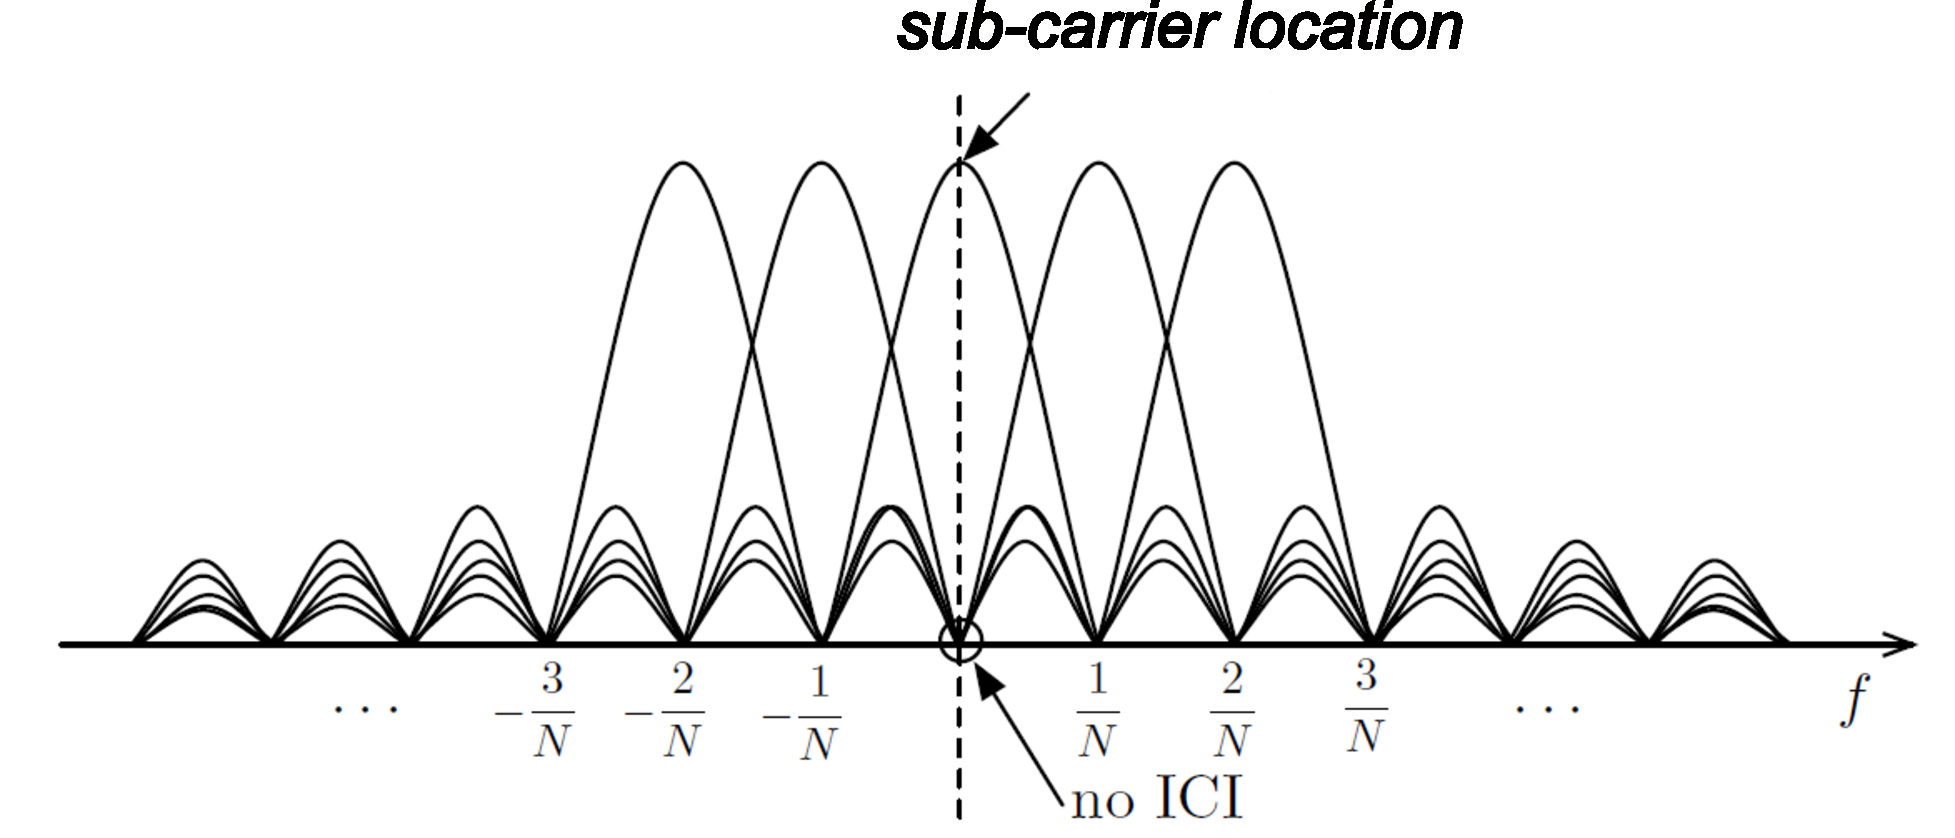
\includegraphics [width=0.8\columnwidth] {Figures/OFDM-subcarrier.pdf} }
	\caption{The spectrum of subcarriers in OFDM \cite{farhang2008signal}}
	\label{fig:OFDM-subcarrier}
\end{figure}

An OFDM symbol signal can be expressed at baseband by a sum of modulated complex exponentials as:

\begin{eqnarray}
\label{equ:OFDMsignal}
s(t) = \sum_{k=0}^{N-1} X_k e^{i2\pi\Delta ft},
\end{eqnarray}
where $X_{k}$ represents a data modulated symbol such as a BPSK, QPSK, or QAM symbol, and is a complex number modulated by the $kth$ subcarrier of $N$ subcarriers and $\Delta f$ is the subcarrier spacing. 
Sampling this OFDM symbol signal with sampling period of $T_S$ is expressed as:

\begin{eqnarray}
\label{equ:sampledOFDMsignal}
s(nT_S) = \sum_{k=0}^{N-1} X_k e^{i2\pi\Delta fnT_S},
\end{eqnarray}
A sample of the OFDM signal is equivalent to an inverse N-point discrete Fourier transform (IDFT), taking $X_{k}$ as a discrete point in the frequency domain. 
Inversely, the sampled OFDM symbol signal can be demodulated using the discrete Fourier transform (DFT). The OFDM modulation and demodulation are hence performed by computing the IDFT and DFT, respectively, expressed as:

\begin{eqnarray}
\label{equ:sampledOFDMsignal}
s[n] = \frac{1}{N}\sum_{k=0}^{N-1} X[k] e^{i2\pi\frac{k}{N}n},
\end{eqnarray} 
\begin{eqnarray}
\label{equ:sampledOFDMsignal}
X[k] = \sum_{n=0}^{N-1} s[n] e^{-i2\pi\frac{k}{N}n},
\end{eqnarray} 

In order to achieve efficient computation, The inverse Fast Fourier Transform (IFFT) and Fast Fourier Transform (FFT) are implemented in an OFDM system to modulate and demodulate the signal instead of the IDFT and DFT, respectively. These optimised algorithms generally rely on the number of points, and hence carriers, being a power of 2.

%---------------------------------------------------------------------------------
\subsection{Cyclic Prefix}
%---------------------------------------------------------------------------------

When transmitting OFDM symbols over a delay-dispersive multi-path channel, the received signal is the linear convolution of the transmitted symbol with the channel impulse
response (CIR) 

\begin{eqnarray}
\label{equ:sampledOFDMsignal}
y[n] = h*s[n],
\end{eqnarray} 

where $h$, assuming it has a length of $L$, denotes the equivalent impulse response of the channel. and $*$ is the convolution operation. 
The received symbols $y[n]$ are the result of convolution between CIR $h$ and transmitted symbols $s[n]$ which has a length of $N$.
So,  $y[n]$ has a length of $N+L-1$.
In addition, the received signal is obtained by concatenating the received OFDM symbols. 
Because the received symbols, having a length of $N+L-1$, are overlapped with the adjacent received symbols, adding the overlap of adjacent received symbols leads to the introduction of the Inter Symbol Interference (ISI) in the received signal shown in Fig.~\ref{fig:CIR-noCP}.


\begin{figure}
	\centerline{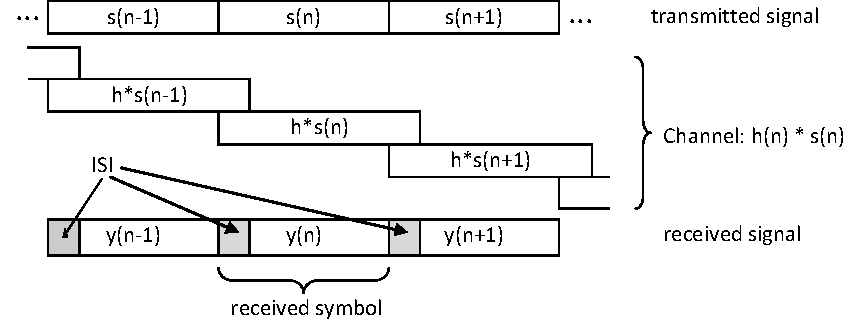
\includegraphics [width=0.8\columnwidth] {Figures/CIR_noCP.pdf} }
	\caption{OFDM transmission without cyclic prefix results ISI among adjacent symbol}
	\label{fig:CIR-noCP}
\end{figure}

In order to avoid ISI, a guard interval (or cyclic prefix), having a length of $L_{CP}$, has to be added before each OFDM symbol as demonstrated in Fig.~\ref{fig:CIR-CP}. 
If the length of CIR, $L$, is smaller than that of the guard interval, $L_{CP}$, adding the overlap of adjacent received symbols will not interfere with the succeeding received OFDM symbol. 
The ISI is hence missing in the received symbol.  
The guard interval, adopted in standards, can be commonly performed by a copy of the last $L_{CP}$ samples of the symbol as shown in Fig.~\ref{fig:CP}, that is called a cyclic prefix (CP)

\begin{figure}
	\centerline{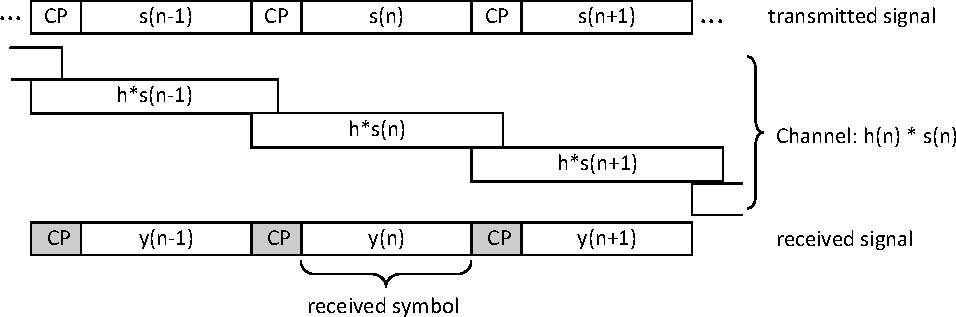
\includegraphics [width=0.8\columnwidth] {Figures/CIR_CP.pdf} }
	\caption{OFDM transmission with cyclic prefix avoids ISI among adjacent symbol}
	\label{fig:CIR-CP}
\end{figure}

\begin{figure}
	\centerline{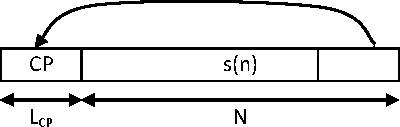
\includegraphics [width=0.8\columnwidth] {Figures/CP.pdf} }
	\caption{Inserting Cyclic Prefix in the OFDM symbol}
	\label{fig:CP}
\end{figure}

In addition, the use of CP also guarantees the orthogonality of subcarriers avoiding the ICI. Performing DFT operation and a single-tap equalizer per subcarrier allows recovery of the transmitted symbols \cite{farhang2008signal}. 

%---------------------------------------------------------------------------------
\subsection{OFDM-based system}
%---------------------------------------------------------------------------------
In the above section, the OFDM modulation technique was presented, and inserting CP was introduced to improve the performance of OFDM in multi path channel. 
A OFDM-based system model can be equivalently considered as shown in Fig.~\ref{fig:OFDM-model}.

\begin{figure}
	\centerline{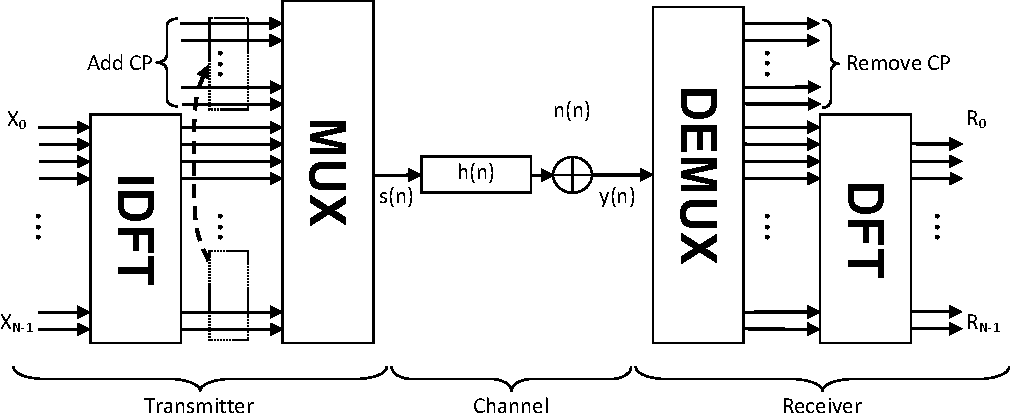
\includegraphics [width=0.8\columnwidth] {Figures/OFDM-model.pdf} }
	\caption{the OFDM system model}
	\label{fig:OFDM-model}
\end{figure}

In the transmitter, the data modulated symbols $X[n]$ are grouped in a blocks of $N$ sub-carrier symbols known as an OFDM symbol, expressed by a vector $X[n]=(X[1], X[2], ..., X[n])^T$. 
Next, the OFDM symbol signal in the time domain is modulated by performing IDFT on each OFDM symbol, and a cyclic prefix of length $L_{CP}$ is inserted at the begin of OFDM signal. 
So, the complex signal of $m$, the OFDM-symbol in baseband discrete time, can be expressed as
\begin{eqnarray}
\label{equ:OFDMsymbol}
s_{m}[n] = \frac{1}{N} \sum_{k=0}^{N-1}X[k]e^{i2\pi k\frac{n-L_{CP}}{N}},
\end{eqnarray} 

where $n$ is the discrete time index, $m$ denotes the index of the OFDM symbol. 
The complete transmitted signal in the discrete time domain, $s[n]$, is given by the concatenation of all OFDM symbols, $s_{m}[n]$,

\begin{eqnarray}
\label{equ:OFDMsignal}
s[n] =  \sum_{m=0}^{\infty} s_{m}[n-m(N+L_{CP})],
\end{eqnarray} 

When transmitting OFDM signals over a multi-path channel, the received signal is obtained through the linear convolution of the transmitted symbol with CIR $h[i]$ and adding additive white Gaussian noise (AWGN) $n$. 
Assuming that the synchronisation between the transmitter and receiver are perfectly achieved, the channel fading is slow enough to consider as a time invariant channel during one OFDM symbol interval, and the length of cyclic prefix is longer than that of CIR ($h[i] = 0$ for $i < 0 i > L_{CP}-1$), 

\begin{eqnarray}
\label{equ:OFDMchannelsignal}
y[n] =  \sum_{i=0}^{L_{CP}-1} h[i]s[n-i] + n[n],
\end{eqnarray} 

In the receiver, the incoming samples $y[n]$ are synchronously  grouped into block of OFDM symbols and then the cyclic prefix in each OFDM symbol is removed. 
The received symbols can be expressed in a vector $y_{m} = (y_{1}, y_{2}, . . . )$ , with $y_{m}[n]=y[m(Nc+Ncp)+Ncp +n]$.
The received data symbols associated with $m^{th}$ OFDM symbol $R_{m}[n]$ are retrieved by performing a $N$-point DFT:

\begin{eqnarray}
\label{equ:receiveOFDMsymbol}
R_{m}[n] =  \sum_{n=0}^{N-1} y_{m}[n]e^{-i2\pi \frac{nk}{N}},
\end{eqnarray} 

\begin{figure}
	\centerline{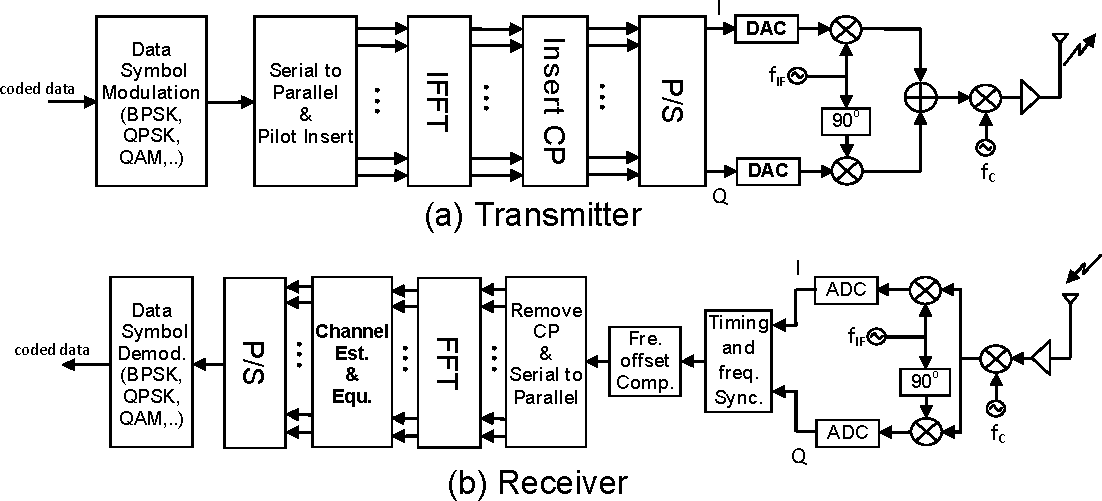
\includegraphics [width=0.8\columnwidth] {Figures/OFDM-block.pdf} }
	\caption{The block diagram of OFDM-based RF systems}
	\label{fig:OFDM-block}
\end{figure}

Fig.~\ref{fig:OFDM-block} presents the common block diagram of an OFDM-based RF system.
OFDM is perform in the baseband, IFFT and FFT blocks are used to compute IDFT and DFT for OFDM modulation and demodulation, respectively.
In the transceiver, the channel coded data from higher abstracted layers is modulated to data symbols (BPSK, QPSK, QAM, ...). The data symbols are then grouped together with the pilots to form $N$ FFT points in parallel.
After performing IFFT, the CP is inserted, and then the OFDM samples are serialised and split in to in-phase (I) and quadrature (Q) channels corresponding to the real and imaginary parts of  the OFDM sample. 
The digital to analogue converted signals of I and Q channels are modulated by an intermediate frequency, $f_{IF}$, then the signal is up-converted to high frequency by an RF carrier, $f_{C}$. 
Before transmitting, the signal should be amplified by an low noise amplifier (LNA).

In the receiver, after down-converting and IQ demodulation, the signal is sampled. The samples are formed from I and Q channels corresponding to the real and imaginary parts of the OFDM sample.
The timing and frequency synchronisation blocks detect the frame, recover timing of the frame and estimate the frequency offset. 
The received samples are then compensated by estimated frequency offset in the discrete time domain. 
After demodulating an OFDM symbol using FFT, estimating the channel and then channel equalisation as well as phase error compensation are performed to improve performance.
The block of parallel samples in an OFDM symbol is serialised to data symbol sequences that are then demodulated, and coded data is sent to higher abstracted layers to decode.

%---------------------------------------------------------------------------------
\subsection{Evaluating OFDM}
%---------------------------------------------------------------------------------

The main advantages of OFDM are its spectrally efficient usage and robustness against multi path propagation.
This makes OFDM suitable for high performance wireless applications. 
OFDM uses multiple sub-carriers which are overlapped with other subcarriers in the frequency domain, resulting in greater spectral efficiency than FDM. 
Performing OFDM is equivalent to splitting a data stream into several parallel low-rate streams before transmission.
This makes the OFDM signal more robust against fading when transmitted through the channel. 
Thanks to the cyclic prefix, the ISI and ICI caused by the multi-path channel can be eliminated. 
The CP creates a guard period for an OFDM symbol, which should be longer than the CIR to ensure no ISI.
Repeating samples of the OFDM symbol in a guard period, the CP helps to maintain the orthogonality of subcarriers avoiding the ICI. 
Thus, performing the DFT and a single-tap equalizer per subcarrier allows recovery of the transmitted symbols.

On the other hand, OFDM has some disadvantages. 
Firstly, an OFDM signal is the sum of multiple modulated sub-carriers, and thus suffers a high peak-to-average power ratio (PAPR). 
This results in demand on high power and wide range linearity in amplifiers increasing the cost of OFDM-based systems.
Secondly, the usage of guard period reduces bandwidth efficiency of OFDM.
Last but not least, OFDM performance is sensitive to receiver synchronisation. Frequency offset causes inter-subcarrier interference and errors in timing synchronisation can lead to inter-symbol interference.
Much effort is needed to improve the accuracy of both frequency and time synchronizers for OFDM.

%-------------------------------------------------------------------------------------------------------------------------------------------------------------------------------------------------------------------------------------------------------------
\section{Multiple Standard Cognitive Radios}
%-------------------------------------------------------------------------------------------------------------------------------------------------------------------------------------------------------------------------------------------------------------

The spectral resource demands of wireless telecommunication systems continues to increase. %Practically, radio spectrum is not fully usage regarding to its capacity by regulatory and license processes for spectral allocation.
Cognitive Radios (CRs), that have ability to adapte to channel conditions, ensuring effective spectrum usage, are an important technology for achieving this. 
They are designed to transmit in currently unused spectrum without causing harmful interference to primary users (PUs) or incumbent users (IUs).
Apart from the critical issues of spectrum sensing and band allocation, the lower priority of secondary users (SUs) raises a challenge in terms of transmission capability and quality of service in cognitive radios. 
When the spectrum allowed for a CR system is fully occupied by PUs and IUs, the transmission of CRs can be blocked. 
Multiple Standard Cognitive Radios (MSCRs) are able to operate in multiple frequency bands with different specified standards.
MSCRs are hence a more flexible generalisation of CRs as they can operate across different bands and standards.

%Most practical CRs are built using powerful general purpose processors to achieve flexibility through software, but they can still fail to offer the computational throughput required for advanced modulation and coding techniques and they often have high power consumption.
%GNU Radio~\cite{gnuradio} has been a widely used platform in academia. 
%It is a software application that runs on a computer or an embedded ARM processor platform, e.g. on the Ettus USRP E100. 
%Computational limitations mean that while it has been successful for investigating CR ideas, it is not feasible for implementing advanced embedded radios using complex algorithms.
%Other software based frameworks like Iris~\cite{Sutton2010}, have some limited support for FPGAs but suffer from poor bandwidth between software and hardware.

%In an application area with fast moving standards and requiring support for multiple standards, custom ASIC implementation is prohibitive.
%Delorme et al.~\cite{Delorme2008} presented a heterogeneous reconfigurable hardware platform for Cognitive Radio. 
%It can adapt its hardware structure to support standards like GSM, UMTS, wireless LAN. 
%Most processing components run as embedded software on the nodes in a network on chip, while the channel coder and the mapping of the RX chain are implemented inside an FPGA. 
%Partial reconfiguration is used to switch the channel coder from one context to an another depending on SNR. 
%A processor manages data movement between the different processors, the ASIC, and the FPGA. The need for a large data buffer and inefficient data transfer mechanisms lead to increased power consumption and reduced throughput.
%There are few studies on FPGA based platforms for radio implementation. 
%KUAR~\cite{Minden2007} is a mature radio platform built around a fully-featured Pentium PC with a Xilinx Virtex II FPGA. 
%The baseband processing is accelerated on FPGA and only limited for NC-OFDM signal based on the IEEE 802.16 standard.
%Projects at Virginia Tech~\cite{athanaswires} have shown dynamically assembled radio structures on FPGAs, where the target radio system is defined at a high-level with datapaths connecting relatively large functional modules. 
%The modules are wrapped, and each of them consists of a PR module with complied partial bit-streams stored in dynamic library. 
%Using PR eliminates the need for run time compilation, but affording flexibility . 
%A flexible radio controller can insert and remove compiled modules to adapt to current conditions.

Multi-carrier modulation techniques offer an ideal opportunity for such systems due to their regularity and parameterisation. OFDM and Filter Bank Multi Carrier (FBMC) are two types of multi-carrier modulations. OFDM modulation has been the dominant technique adopted for many standards and has been investigated in terms of spectral sensing and carrier allocation for CRs. 
Furthermore, OFDM system implementation is simple, low cost, and can be effectively parameterised in comparison to FBMC systems. OFDM is a suitable candidate for a MSCR system. The advantages of coupling OFDM modulation with an FPGA platform are investigated for the feasibility of implementing the proposed MSCR system. 
The flexibility requirement of a MSCR is to support existing standards like 802.11, 802.16, and 802.22, as well as supporting future OFDM-based standards.

A feasible OFDM-based MSCR requires the ability to switch baseband processing from one standard to another. This means that the system needs to rapidly adapt its functionality to perform variable numbers of FFT/IFFT operations, insert CP of configurable length, and handle differend pilot vectors as well as different preambles. The hardware implementation of an OFDM-based MSCR can be based on the original architecture of an OFDM system illustrated in Fig.~\ref{fig:OFDM-block}. However, each sub-module of the system needs to be designed to perform with all parameters of the supported standards. This results in significantly increasing system complexity as well as reconfiguration time.   

%One way this can be done is for separate implementations of each standard to be implemented as partial bitstreams which are swapped at runtime. However, a large monolithic bitstream requires a longer reconfiguration time. Our proposed approach uses a finer granularity. Each module in the processing chain is investigated and commonalities across standards are analysed. For modules requiring only minor modifications, parameterised versions are created. For those that require significant changes, PR can be used on a per-module level. As a result, when switching from one standard to another, only part of the FPGA needs to be reconfigured.

Beside the challenge of long configuration time for MSCR, there are two key challenges of the baseband related to the synchronizer and spectral shaper. OFDM systems typically tolerate a small carrier frequency offset (CFO) leading to strict constraints on the design of the RF front-end. In an MSCR system, the RF front-end should access a wide range of frequencies depending on the standard in operation. Such a precise and yet wide ranging frequency requirement makes the RF front-end design difficult if not impossible or require very expensive components.
CRs also demand small spectral leakage for both in-band and out-of-band transmitted signals to avoid causing harmful interference to primary users, while OFDM signals have intrinsically large side lobes leading to a potentially large degree of spectral leakage. 
Flexibility in the baseband can allow a frequency guard extending technique to achieve spectral leakage requirements.

The interface to the higher layer processing is another important factor. Many hardware radio platforms are extremely difficult to design for or to modify. Hence, only hardware experts can use them. While detailed optimisation of low level blocks is important, providing a general interface for implementing higher layer processing is also important. This ensures that radio experts may use the system to investigate cognitive radio techniques without the need for specific advanced low-level FPGA expertise.


%-------------------------------------------------------------------------------------------------------------------------------------------------------------------------------------------------------------------------------------------------------------
\section{OFDM Synchronisation}
%-------------------------------------------------------------------------------------------------------------------------------------------------------------------------------------------------------------------------------------------------------------

OFDM performance is sensitive to receiver synchronisation. 
Frequency offset causes inter-subcarrier interference, and errors in timing synchronisation can lead to intersymbol interference. 
Therefore, synchronisation is critical for good performance in OFDM systems. 
There are two main errors implicit in synchronisation: sample clock timing offsets and carrier frequency offsets.
In order to obtain good synchronisation performance, timing offsets and frequency offsets must be studied in terms of their cause and effect on the degradation of OFDM received data symbols.
Additionally, there are issues of common phase error (CPE), generated from clock jitter and phase noise, that causes a random rotation of the entire signal constellation.
This must also be taken into account and compensated for in order to achieve good performance.

%---------------------------------------------------------------------------------
\subsection{Timing Offsets}
%---------------------------------------------------------------------------------

When sampling a signal at the receiver, the different times of sampling between samples in the receiver and transmitter are referred as timing error.
In a single carrier system, the symbol clock in the transmitter can be recovered at the receiver using a phase-lock loop (PLL) \cite{farhang2008signal}. 
This can correct a timing error in the receiver relatively easily.

In OFDM, however, timing errors can be considered in two categories: fractional and integer. 
Fractional timing error, that is errors that are smaller than one sample period, are caused by different phases between the sampling clock of the analogue to digital converter (ADC) in the receiver and the phase of the transmitted signal, while integer timing error is that which is greater than one sample period, causing index shifting, or offset, in the sample sequence.

The timing error in the time domain is equivalent to a phase rotation in the frequency domain expressed in Equ. (\ref{equ:timingoffset}),

\begin{eqnarray}
\label{equ:timingoffset}
               s (t - \tau )   \Leftrightarrow  e^{-i2\pi f\tau} R(f),
\end{eqnarray}	
where $\tau$ denotes timing error resulting in a phase shift of $e^{-i2\pi f\tau}$. 
$s(t)$ is the received signal in the time domain, and $R(f)$ is the spectrum of $s(t)$ in the frequency domain.
The phase shift is proportional to both time errors and the frequency of carriers.
In the case of multi-carriers with increasing frequency, the phase shift is increased according to the carriers leading to the phase rotation of subcarriers.
Carrier rotations caused by fractional timing error $\Delta t$ like that caused by fading can be estimated by a channel estimator and compensated for after performing the DFT,
\begin{eqnarray}
\label{equ:rotationcompensation}
               \widehat{R[n]} = R[n] e^{\frac{i2\pi n \Delta  t}{N}},
\end{eqnarray}
where $R[n]$, $\widehat{R[n]}$ denotes received data symbols before and after compensation, respectively. $\Delta t$ is estimated phase rotation, and N is the number of sub-carriers.

Moreover, the received samples in the receiver are synchronously grouped into blocks of OFDM symbols.
Integer timing errors lead to a symbol timing offset (STO) referring to the difference between correct sample index and the actual sample index of received samples that causes a misaligned window for DFT demodulation in the receiver.
If the timing offset is late, the samples of the following symbol are used for the current symbol, resulting in ISI and hence degrading the performance of the OFDM system. The effect of ISI caused by later timing offsets on the OFDM received symbol is illustrated in Fig.~\ref{fig:Timingoffsetconstellation}(a) and Fig.~\ref{fig:Timingoffsetconstellation}(c).
If the timing offset is early, some samples in the CP of the current symbol are used to calculate the DFT, leading to sub-carrier rotation expressed in Equ.\ref{equ:timingoffset} in the frequency domain.  
The effect of sub-carrier rotation caused by earlier timing offsets on the OFDM received symbol is illustrated in Fig.~\ref{fig:Timingoffsetconstellation}(b) and Fig.~\ref{fig:Timingoffsetconstellation}(d).

\begin{eqnarray}
\label{equ:rotationcompensation}
              s[n - \mathit{t_{off}}]  \Leftrightarrow R[n] e^{\frac{i2\pi n \mathit{t_{off}}}{N}},
\end{eqnarray}
where $s[n]$, $R[n]$ denotes received data symbols in the timing domain and the frequency domain, respectively. $\mathit{t_{off}}$ is a timing offset, and N is the number of sub-carriers.

\begin{figure}
	\centerline{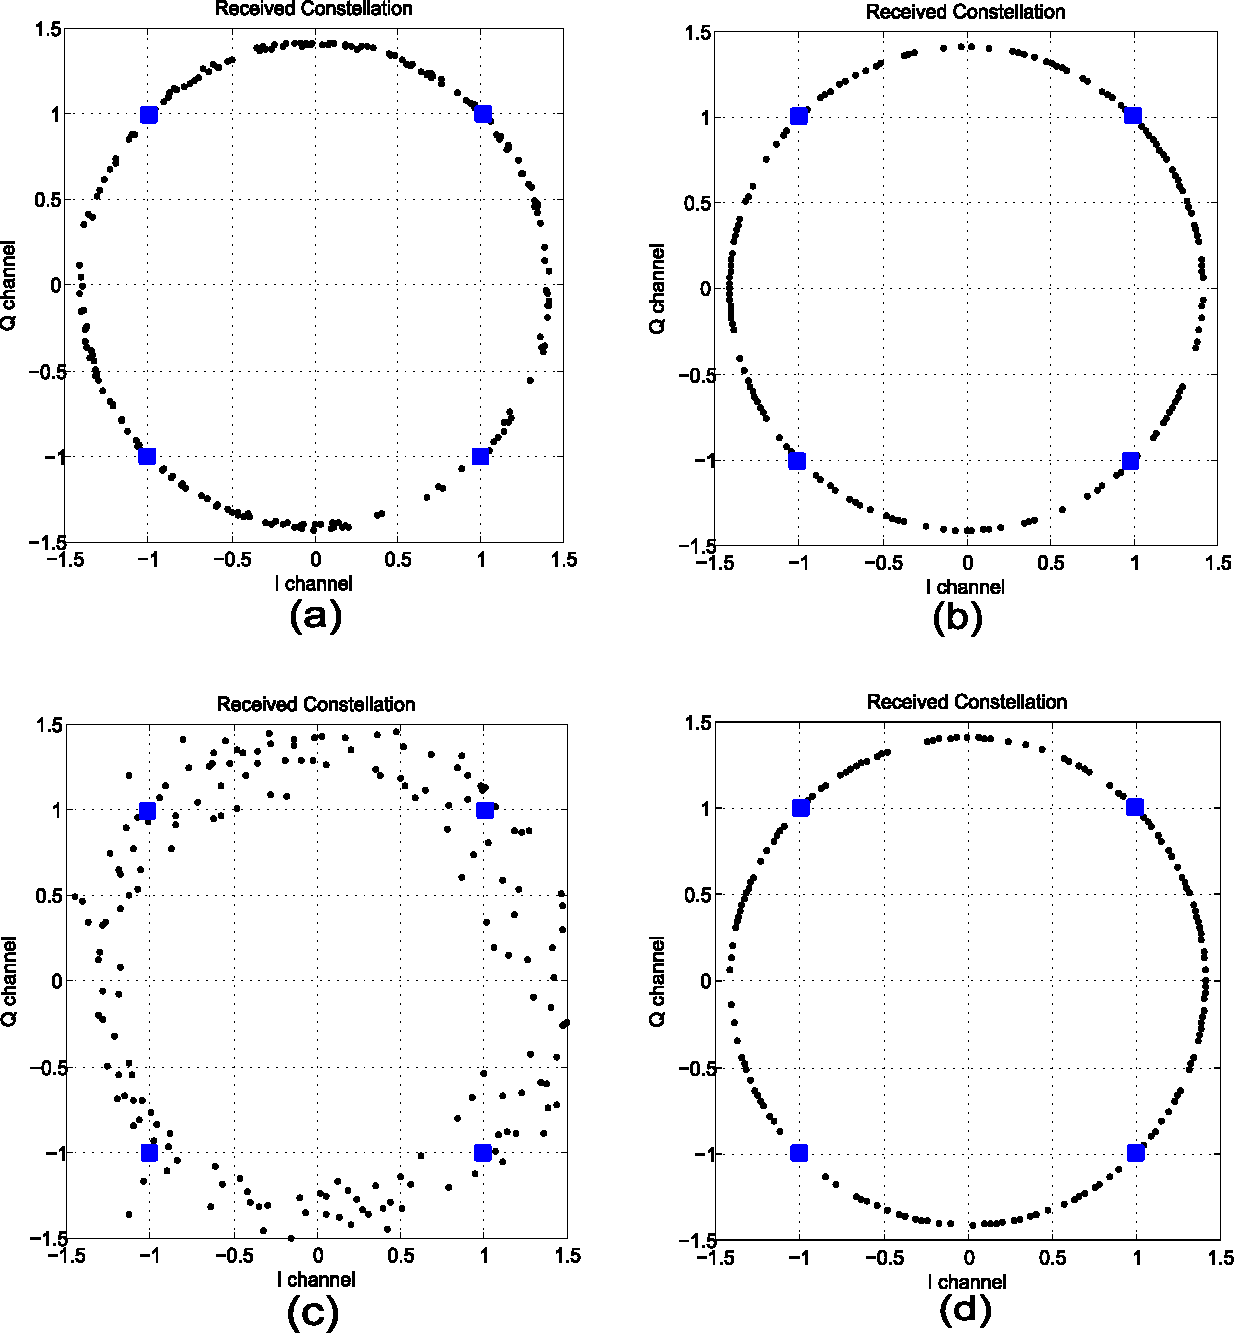
\includegraphics [width=0.8\columnwidth] {Figures/timeoff.pdf} }
	\caption{OFDM received symbol with timing offets of -1, 1, -5 and 5 in a, b, c, d, respectively.}
	\label{fig:Timingoffsetconstellation}
\end{figure}

Fig.~\ref{fig:Timingoffsetconstellation} illustrates the effect of timing offset on a single 256 subcarrier OFDM symbol utilizing QPSK subcarriers (based on the IEEE~802.16).
As can be seen, the earlier timing, for instance timing offsets of 1 and 5, shown respectively in Figs.~\ref{fig:Timingoffsetconstellation}(b) and~\ref{fig:Timingoffsetconstellation}(d), cause a carriers rotation similar to that of fractional timing errors, and fading that can be estimated by a channel estimator.
However, the later timing, for instance timing offsets of 1 and 5, as shown in Figs.~\ref{fig:Timingoffsetconstellation}(a) and~\ref{fig:Timingoffsetconstellation}(c), lead to ISI that prevents the OFDM constellation from being recovered. 
Therefore, timing synchronisation is required to correct the timing offset, and avoid ISI.

%---------------------------------------------------------------------------------
\subsection{Frequency Offset}
%---------------------------------------------------------------------------------

CFO refers to a difference in frequency between the receiver clock with respect to the `correct' frequency of carriers in a transmitted OFDM symbol. 
CFO is introduced by an imperfect clock in the RF front-end part, as well as by frequency variation caused by the Doppler effect when a signal is transmitted through a frequency selective channel. 
This leads to the misalignment of sampling in sub-carriers in the frequency domain that causes a loss of orthogonaltity because at the point of frequency offeset in the sub-carrier, the other sub-carriers are not null as expected (shown in Fig.~\ref{fig:OFDM-subcarrier-freoff}).


\begin{figure}
	\centerline{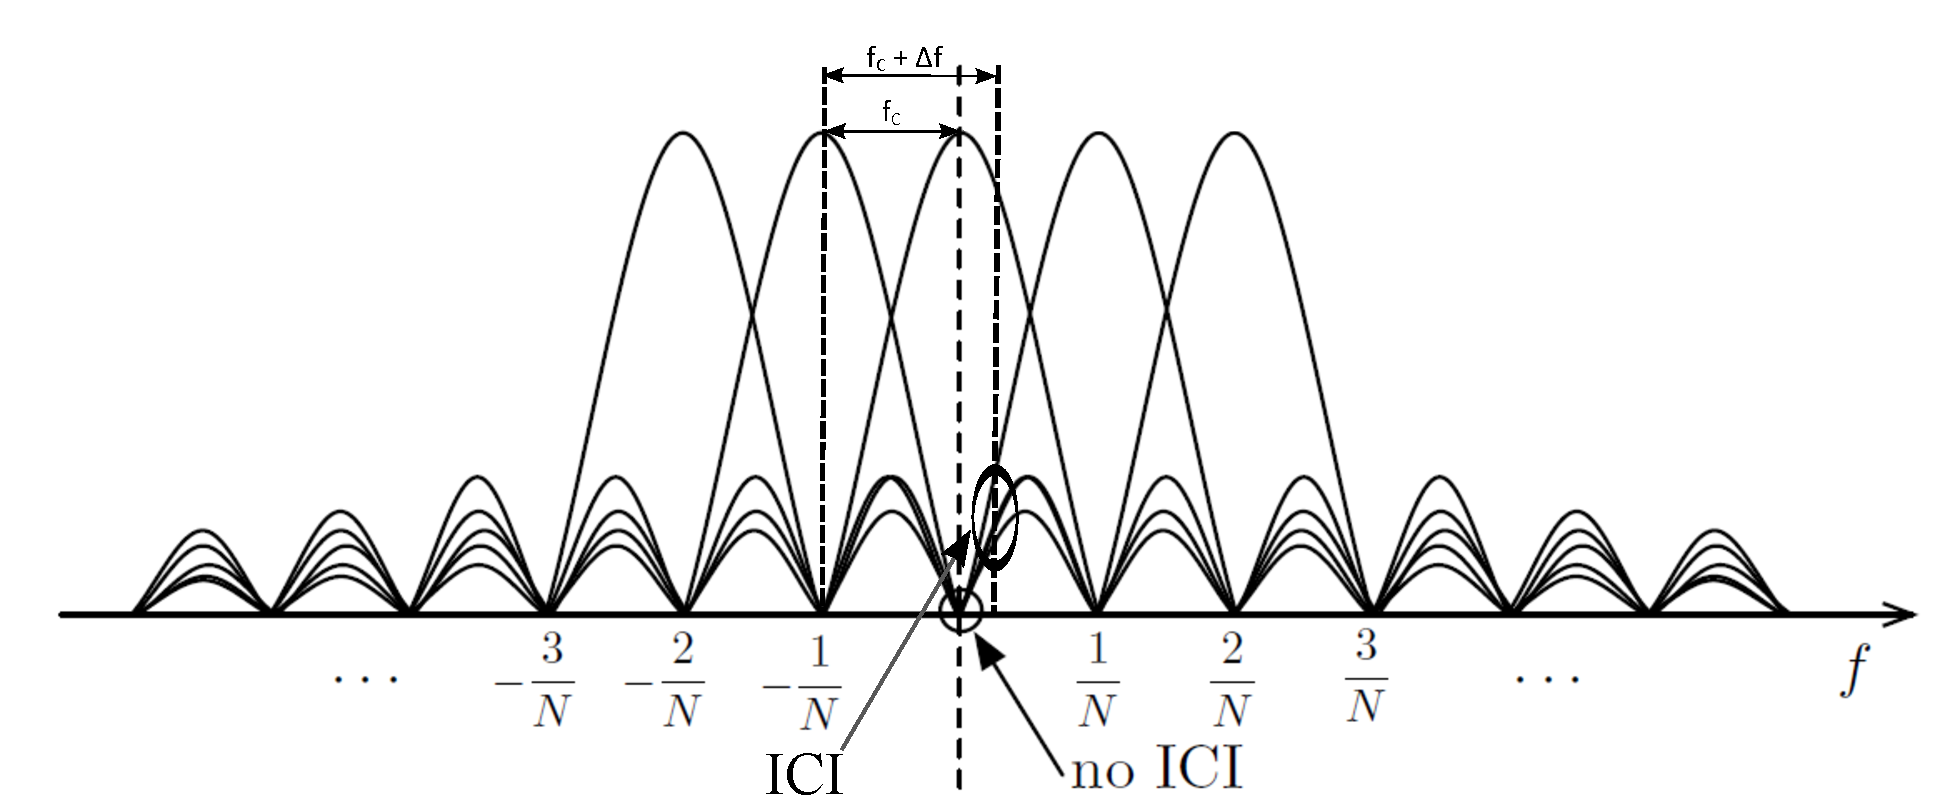
\includegraphics [width=0.8\columnwidth] {Figures/OFDM-subcarrier-freoff.pdf} }
	\caption{Inter carrier interference (ICI) caused by frequency ofsset $\Delta f$.}
	\label{fig:OFDM-subcarrier-freoff}
\end{figure}

With no frequency offset, the frequency bin of the DFT will be sampled at the value at the peak of each subcarrier, $sinc(x)$ pulse, and other adjacent pulses are null at this point. 
However, if frequency offset is introduced, the frequency bin of the DFT will sum the energy from other sub-carriers. 
This means that the adjacent subcarrier introduces an interference component resulting in ICI. 

As can be seen, the adjacent subcarrier introduces an interference component that is about half the amplitude of the subcarrier of interest. 
All other subcarriers introduce an interference component of much lower amplitude. 
This is known as a loss of orthogonality, and must be compensated for in order to properly demodulate the OFDM symbol.
The effect of CFO can be easily considered in the time domain by taking an inverse Fourier transform expressed as follows:

\begin{eqnarray}
\label{equ:}
             R(f - \Delta f) \Leftrightarrow  e^{i2\pi \Delta ft} s(t),
\end{eqnarray}	

In the discrete time domain, the signal sample sequence can be expressed: 
\begin{eqnarray}
\label{equ:}
            s[n]' = s[n] e^{\frac{− i2\pi \Delta fn}{N}},
\end{eqnarray}
where $s[n]'$ and $s[n]$ are the frequency offset samples and the original samples, respectively.
$\Delta f$ denotes the frequency offset, and $N$ is the number of subcarriers. 

The effect of frequency offset is shown in Fig.~\ref{fig:freoff_1sym}. Each plot illutrates the constellation of QPSK symbols demodulated from one 256 sub-carrier OFDM symbol based on the IEEE~802.16 standard.

\begin{figure}
	\centerline{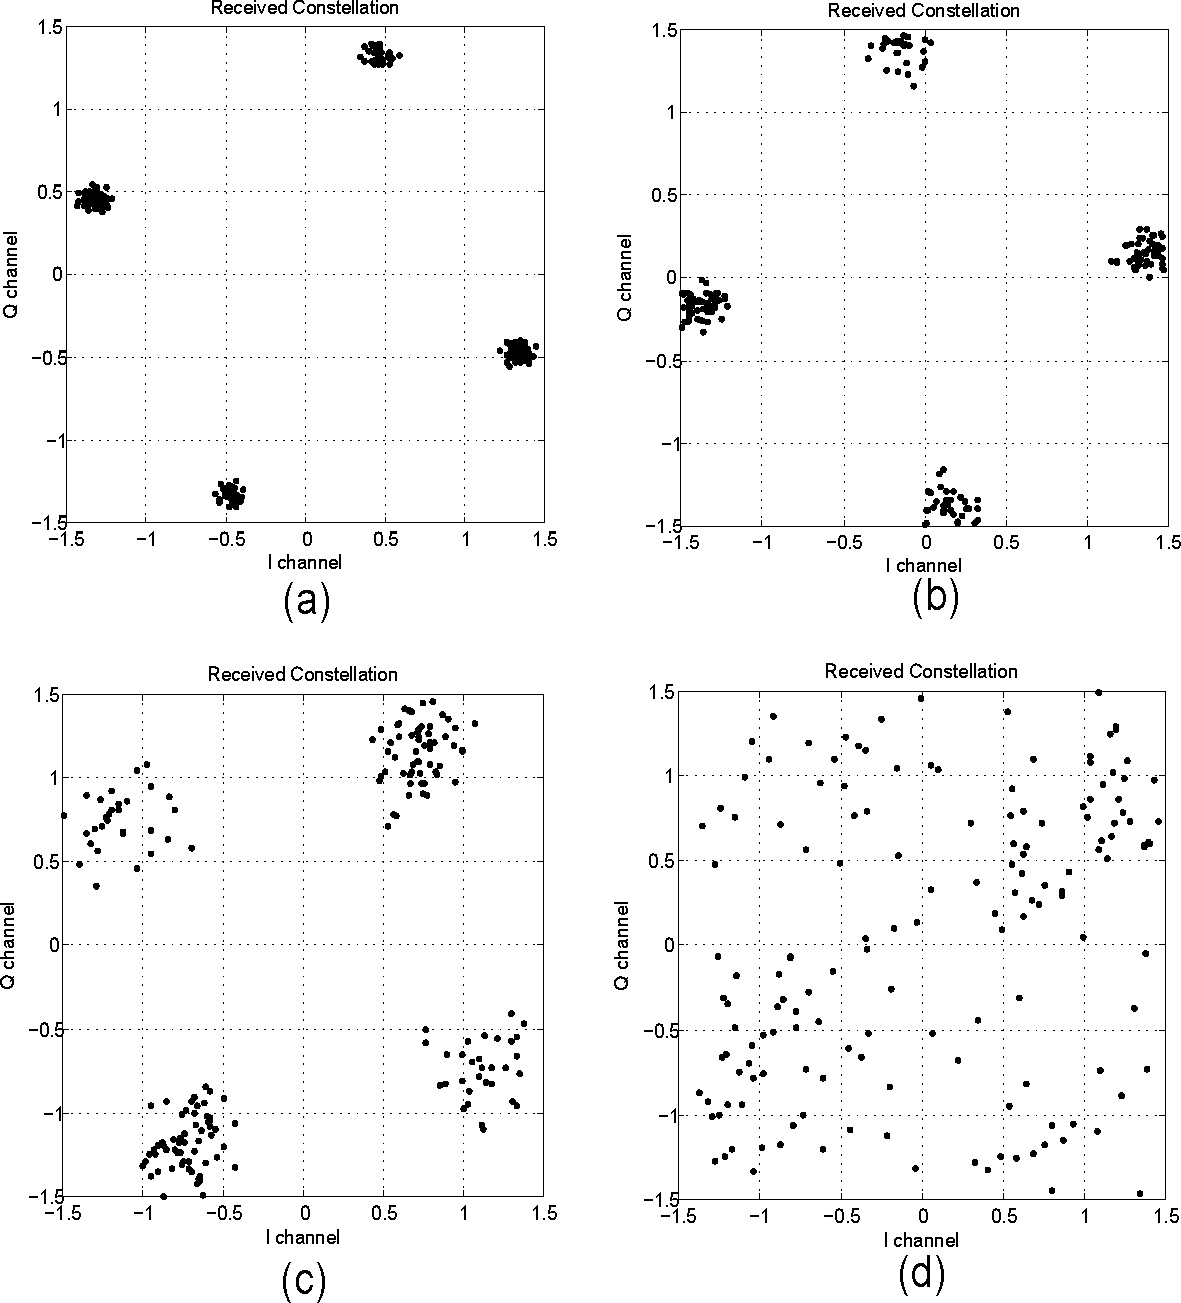
\includegraphics [width=0.8\columnwidth] {Figures/freoff_1sym.pdf} }
	\caption{The constellations of OFDM received symbol with frequency offets of 0.025, 0.5, 0.1 and 0.25 sub-carries spacing in a, b, c, d, respectively.}
	\label{fig:freoff_1sym}
\end{figure}

As can be seen, OFDM performance is sensitive to even small frequency offsets. 
The effect of CFO causes dispersion, similarly to AWGN, and also phase rotation in the QPSK constellation demodulated from OFDM symbol.
If multiple data symbols are transmitted in a packet, the phase rotation of each OFDM symbol increases, and even small CFO will lead to a large drift of constellation points, shown in Fig.~\ref{fig:freoff_5sym} degrading the performance of demodulation. CFO must be estimated and compensated for, in order to properly demodulate the OFDM symbol.

\begin{figure}
	\centerline{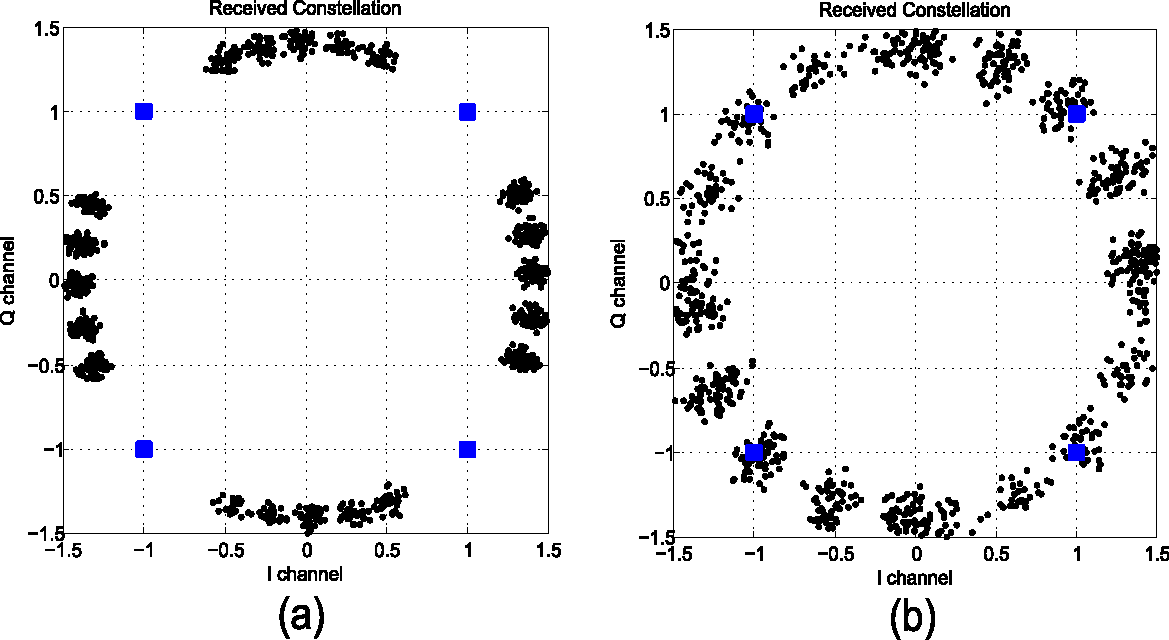
\includegraphics [width=0.8\columnwidth] {Figures/freoff_5sym.pdf} }
	\caption{The constellations of 5 consecutive OFDM received symbols with frequency offets of 0.025 and 0.05 in a, b respectively.}
	\label{fig:freoff_5sym}
\end{figure}

%---------------------------------------------------------------------------------
\subsection{Phase Noise}
%---------------------------------------------------------------------------------

The intrinsic imperfection of the local clock at the RF front-end of a receiver or clock jitter of an ADC may introduce a parasitic phase noise which can affect the performance of baseband data symbols, such as QPSK, QAM, ..., during demodulation.
Phase noise can be considered in two different parts: common phase error and inter-carrier interference \cite{Armada1998}. The effect of phase noise can be expressed in the discrete time domain as:
\begin{eqnarray}
\label{equ:}
            s[n]' = s[n] e^{i\phi[n]},
\end{eqnarray}	
where $s[n]’$ and $s[n]$ are the frequency offset samples and the original samples, respectively.
$\phi[n]$ denotes the phase noise.

If the phase noise is varying more slowly than the OFDM symbol interval, it can be considered a constant phase term added to each sample resulting in CPE \cite{Armada1998}. 
However, if the phase noise is varying much faster than the OFDM interval, different phase noise is added to each sample causing the loss of orthogonality, and thus, intercarrier interference.  
Fig.~\ref{fig:phasenoise} illustrates the effect of phase noise on baseband data symbol demodulation in an OFDM received symbol and 5 consecutive OFDM received symbols.
\begin{figure}
	\centerline{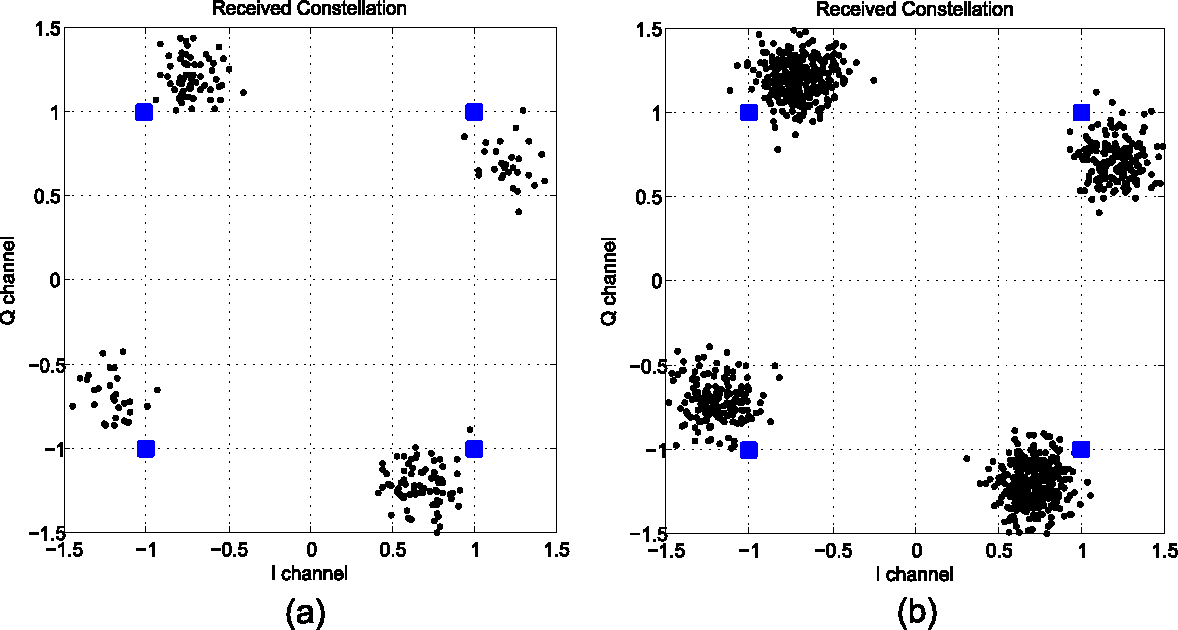
\includegraphics [width=0.8\columnwidth] {Figures/phasenoise.pdf} }
	\caption{The constellations of an OFDM received symbol and 5 consecutive OFDM received symbols with phase noise variance of 0.25 $rad^2$ in (a), (b) respectively.}
	\label{fig:phasenoise}
\end{figure}

As can be seen in Fig.~\ref{fig:phasenoise}, the degradation of OFDM demodulation includes two different phenomena affected by phase noise.
First, the constellations of the data symbol are rotated similarly to the effect of fractional timing error or residual frequency offset.
Second, the constellations of data symbols are dispersed like the effect of AWGN, that causes a loss of orthogonality between the sub-carriers.
However, the difference from the effect of frequency offset will be a constant constellation rotation for all OFDM symbol instead of a different constellation rotation for each symbol in the case of  frequency offset.


%------------------------------------------------------------------------------------------------------------------------------------------------------------------------------------------------------------------------------------------------------------
\section{Shaping OFDM Spectral Leakage}
\label{Ch2:SpecLeak}
%------------------------------------------------------------------------------------------------------------------------------------------------------------------------------------------------------------------------------------------------------------
OFDM modulation techniques have been adopted for many wireless standards as well as enabling technology for cognitive radios.
However, one of their main disadvantages is spectral leakage due to the summation of sinusoidal subcarriers and having been windowed by a rectangular function.
In addition, some recent OFDM-based standards demand very strict requirements on spectral leakage to avoid inter-channel interference.
This raises a significant challenge in how to shape the spectrum of the OFDM signal. 

In 2009, the FCC issued regulatory rules for reusing the television white space (TVWS) spectrum.
IEEE~802.11af was developed under the 802.11 Working Group as a standard that enables a Wi-Fi service in the TVWS spectral regions~\cite{802-11af2013}. 
The scope of the standard is to define amendments to the high throughput 802.11's PHY and MAC layers to meet the requirements for channel access and coexistence in the TVWS regions.
One of the main challenges is the stringent SEM requirements that are mandated by the FCC for these services.. 
The high throughput 802.11 scaled SEM has a large gap between current performance and the required spectral emissions shape for TVWS~\cite{Shellhammer2009}.
For instance, the 802.11 scaled SEM requires an attenuation of 20~dB at the edge of the channel whereas the equivalent this requirement for portable TV band devices (TVBD) is 55~dB.

In 2010, the IEEE defined a standard for PHY and MAC layers~\cite{802-11p2010}, named IEEE~802.11p, for Dedicated Short-Range Communications (DSRC), the wireless channel for new vehicular safety applications through vehicle-to-vehicle (V2V) and Road to Vehicle (RTV) communications.
The PHY in 802.11p is largely inherited from the well-established IEEE~802.11a OFDM PHY, with several changes aimed at improving performance in vehicular environments.
The advantage of building on 802.11a is a potential significant reduction in the cost and development effort necessary to develop the new 802.11p hardware and software.
It also plays an important role in allowing backwards compatibility from 802.11p to 802.11a~\cite{Vandenberghe2011,Fernandez2012}.
Essentially, three changes are made in IEEE~802.11p~\cite{Jiang2008}:
First, 802.11p defines a 10~MHz channel width instead of the 20~MHz used by 802.11a.
This extends the guard interval to address the effects of Doppler spread and inter-symbol interference in a VC channel.
Secondly, 802.11p defines several improvements in receiver adjacent channel rejection performance to reduce the effect of cross channel interference that is especially important in dense vehicle communication channels.
Finally, 802.11p defines four SEMs corresponding to class A to D operations that are specified and issued in FCC~CFR47 Sections 90.377 and 95.1509.
These are more stringent than for current 802.11 radios, in order to improve performance in urban vehicle scenarios.
In addition, 802.11p will operate in the 5.9~GHz DSRC spectrum divided into seven 10~MHz bands. 
This channelization allows the MAC upper layer to perform multi-channel operations \cite{WAVE2010}.
The mechanism allows safety and other applications to occupy separate channels to reduce interference.
The four strict 802.11p SEMs are defined to reduce the effect of ICI between the channels. %, shown in Fig.~\ref{fig:4SEM},
Wu et al. \cite{Wu2013} showed that transmitters on adjacent service channels still cause inter-channel interference (ICI) in the safety channel, even if they satisfy the class C requirement.
Shaping 802.11p  spectral leakage is thus potentially important in helping to eliminate ICI.

Conventionally, there are two methods that can be employed to compress the spectral leakage for OFDM-based system, namely pulse shaping and image spectrum compression. Pulse shaping, recommended in 802.11a, is effective at reducing side lobes. 
Considering an OFDM symbol to have IFFT length and CP length $N$ and $N_{CP}$, respectively, the length of the symbol including its CP is $N_{T} = N + N_{CP}$,
a sample $x[m]$ of the OFDM symbol $(0\leq m \leq N_{T}-1)$ can be expressed in the time domain as,
\begin{equation}
\label{xm}
x[m] = \frac{1}{N}\sum_{k=0}^{N-1} X[k] e^{i2\pi\frac{k}{N}(m-N_{CP})},
\end{equation}
where $X[k]$ denotes the frequency domain representation of the data sub-carriers.
Since OFDM symbol samples are generally transmitted sequentially, this is equivalent to multiplying symbols with a rectangular window function, $p$.
Then the transmitted OFDM samples can be expressed as;
\begin{equation}
\label{equ:xn2}
x[n] = \frac{1}{N}\sum_{l=-\infty}^{\infty} \sum_{k=0}^{N-1} X[k] p[n-l N_{T}] e^{i2\pi\frac{k}{N}(n-N_{CP}-l N_{T})}
\end{equation}
In a conventional OFDM system, the window function, $p(m)$, is rectangular and simply described as;
\begin{equation}
\label{equ:pm}
 p[m] =\begin{cases}1, & m = 0,1, ..., N_{T} \\  0, & otherwise \end{cases}
\end{equation}
In pulse shaping OFDM, the window function, $p[m]$, uses a smooth rather than rectangular pulse resulting in inducing distortion in the subcarriers.
One way to avoid this is to add extending parts, i.e. CP and a cyclic suffix (CS) before and after each conventional OFDM symbol respectively, and to multiply the extended symbol with a smoothing function.
While the CP in conventional OFDM is used as a guard interval, here it is also used for pulse shaping. Pulse shaping extends the  $N_{T}$ length of the OFDM signal by a roll-off factor, $\beta$.
The overhead of extending CS results in spectral loss; overlapping of the CP and CS of consecutive symbols shown in Fig.~\ref{fig:PS} is needed to form a transmitted symbol to reduce this loss, but causes ISI in the overlapped region. Pulse shaping using the overlapping method is effectively equivalent to shortening the OFDM guard interval.
A larger $\beta$ obtains greater compression in spectral leakage but reduces the effective guard interval.
When $\beta N_{T}$ is increased to equal the CP length, the effective guard interval is reduced to zero (no guard interval) to prevent channel-induced ISI.

\begin{figure}[t]
    \centerline{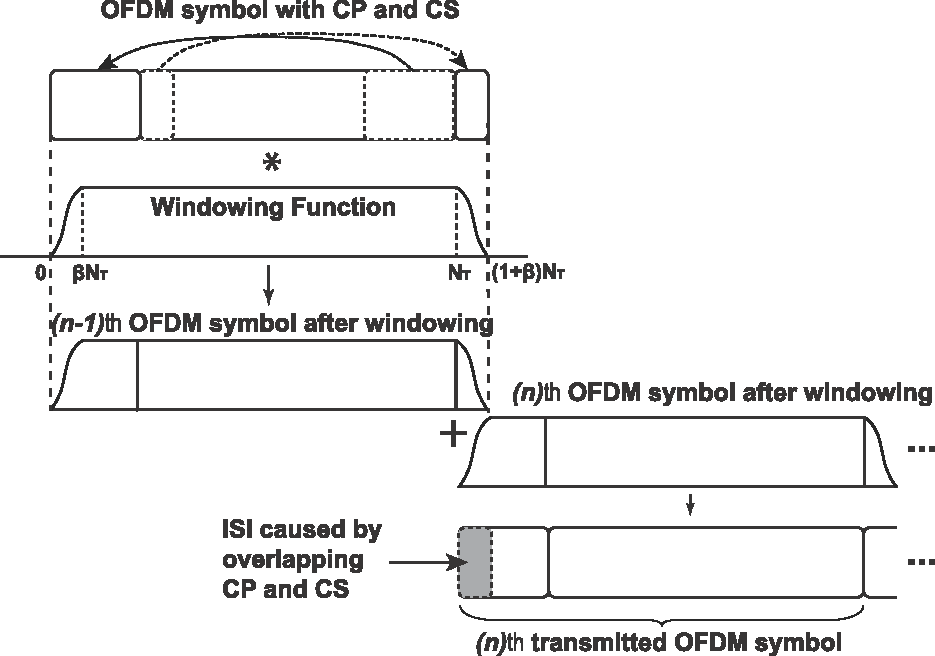
\includegraphics [width=0.9\columnwidth, height=7.5cm] {./Figures/w-ofdm.pdf} }
	\vspace{-2mm}
    \caption{Pulse Shaping operation performed on OFDM symbols.}
    \label{fig:PS}
\end{figure}

Image spectrum compression is implemented as an FIR filter to cancel image spectra.
The Interpolation can be used at baseband to increase sampling frequency, thereby extending baseband bandwidth.
Image spectra are repeats of the original baseband spectrum, present because of interpolation or digital analogue converter (DAC) effects.
On one hand, the narrow band gap between main and adjacent image spectra requires a long impulse response FIR filter.
On the other hand, according to the performance of FIR expressed in (\ref{equ:FIR}), the impulse response of the FIR filter $h$ with length $L_{FIR}$ has a similar effect to the impulse response of the overall channel in terms of inducing ISI.
\begin{equation}
\label{equ:FIR}
y[n] =  \sum_{i=0}^{L_{FIR}-1} h[i]x[n-i] 
\end{equation}

The FIR filter reduces the effective guard interval of OFDM symbols~\cite{farhang2008signal}.
Its design also needs to deal with the tradeoff between the length of filter to avoid ISI and the transition band and attenuation of the filter to meet the requirement of SEMs.

%------------------------------------------------------------------------------------------------------------------------------------------------------------------------------------------------------------------------------------------------------------
\section{Summary}
%------------------------------------------------------------------------------------------------------------------------------------------------------------------------------------------------------------------------------------------------------------

Reducing power dissipation has become a crucial issue in wireless communication systems, especially for portable devices. 
In this chapter, the power consumption of FPGA systems is discussed.
The power estimation and analysis tools of Xilinx are also studied and employed in this research to evaluate the power dissipation of the researched system for power consumption optimisation. 
Some low-power design strategies are suggested.
This chapter also provides the background of OFDM in terms of its mathematical representation and functionality, and then the advantages and limitations of OFDM are also discussed.
The concept of a MSRC based on OFDM techniques is presented. The challenges of implementing the MSCR system are introduced regarding the architecture and its performance.
The synchronisation effects on the OFDM performance are also considered. 
Last but not least, the challenge in terms of OFDM spectral leakage are discussed in case of the strict requirements imposed by recent wireless standards. 

\chapter{Background Literature}
\label{chap:BackgroundLiterature}
%%---------------------------------------------------------------------------------
\chapter{Multiplierless Correlator Design for low-power systems}
\label{chap:multiplierlesscorrelator}
%---------------------------------------------------------------------------------

%---------------------------------------------------------------------------------
\section{Introduction}
%---------------------------------------------------------------------------------
Correlation operators are commonly used to perform synchronisation in OFDM systems.
Auto-correlation based techniques are preferred for implementing  OFDM synchronisation on FPGA because of their lower hardware costs. 
Dick and Harris \cite{Dick2003} reported on the FPGA implementation of an OFDM transceiver. 
Their paper shows that FPGAs, with their highly parallel architecture, are suitable for the implementation of OFDM transceivers.
Wang et al. \cite{Wang2004} also presented an FPGA implementation of an OFDM-WLAN synchronizer. 
In \cite{Wang2004}, the timing synchronisation is obtained by double auto-correlation based on short training symbols that allows a reduction in the hardware cost on FPGA. 
Fort et al. \cite{Fort2003} compared  the performance and complexity of FPGA implementation of auto-correlation algorithms and cross-correlation algorithms.
Results showed that the accuracy of cross-correlation algorithms is better than that of auto-correlation algorithms. 
However, the accuracy of cross-correlation comes at significant hardware cost. 
Despite proposing a new cross-correlator implementation to reduce hardware cost compared to a classic cross-correlation approach, it is still at least 5 times more complex to implement than auto-correlation, due to the fact that several multipliers are required. 

Cross-correlation between received samples and a known preamble can achieve highly accurate timing synchronisation, however, this requires significant resources. 
Multiplierless correlators for timing synchronisation were introduced in \cite{Yip2003}, designed for IEEE 802.11a OFDM frames, based on expressing the correlator coefficients as sums of powers of two that only require shift and add operations. 
The authors identified a correlator that eliminates the need for multiplication, requiring only 26 additions/subtractions per output while maintaining similar synchronisation accuracy to a multiplier-based implementation.

Modern FPGAs contain various resources that can be used to implement cross-correlation.
This chapter presents the design of several correlators for timing synchronisation with preamble symbols based upon IEEE 802.16d. 
We compare designs using specialised DSP Slices to a multiplierless approach on Xilinx Virtex-6 and Spartan-6 FPGA devices. 
Attempting to implement correlation on FPGAs without considering and designing for the underlying architecture is likely to result in an inefficient implementation.
In this chapter, we show optimised designs, built to fit the FPGA architecture, and evaluate performance, timing synchronisation accuracy, resource utilisation, and power consumption, to understand whether a multiplier-based mapping is beneficial when using modern devices. 
%---------------------------------------------------------------------------------
\section{Implementation of correlators}
%---------------------------------------------------------------------------------

The downlink preamble in IEEE 802.16d \cite{IEEE80216} contains two consecutive OFDM symbols as shown in Fig. \ref{fig:pre}.  
The short symbol consists of 4 identical 64-sample fragments in time, preceded by a cyclic prefix (CP). 
This is followed by the long symbol which contains two repetitions of a 128 sample fragment and a CP \cite{IEEE80216}. 

\begin{figure}
	\centerline{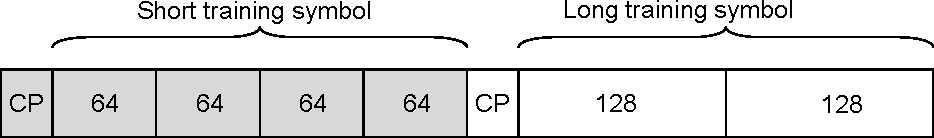
\includegraphics [width=0.7\columnwidth] {figures/Preamble.pdf} }
	\caption{Downlink preamble symbols for IEEE802.16.}
	\label{fig:pre}
\end{figure}

\begin{figure}
	\centerline{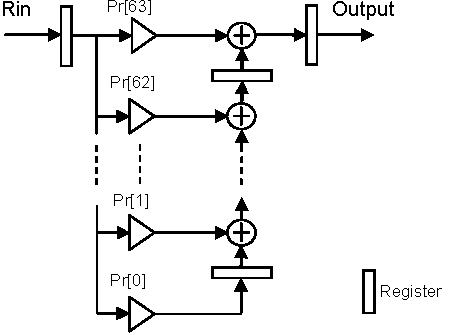
\includegraphics [width=0.5\columnwidth] {figures/structure_correlator.pdf} }
	\caption{Transpose Direct Form of Correlator.}
	\label{fig:str_corr}
\end{figure}


The 64 samples in the short symbol are used to perform cross-correlation with received samples for timing synchronisation. 
Therefore, the correlators are designed to compute cross-correlation with 64 constant coefficients. 
In this chapter, we explore two approaches to implementing such correlators. 
The first is based on Xilinx Virtex-6 FPGA DSP48E1 Slices, the standard approach to such an implementation.
The second is using multiplierless correlation implemented on both a Xilinx Virtex-6 and a low power Xilinx Spartan-6 device.
Both are designed to receive real and imaginary 16-bit samples in Q1.15 fixed point format. 
The output is the sum of 64 coefficient products, each being smaller than unity. 
So, the complex output words are in 21-bit fixed point Q6.15 format. 

If such a design was implemented blindly, with no consideration for the FPGA architecture, the synthesis tools would infer the use of embedded DSP blocks for multiplication, but would likely achieve poor timing due to an inability to optimise the use of the DSP block.
The DSP48E1 primitives on the Virtex-6 FPGAs have additional circuitry within them that enables the design of optimised datapaths, but this must be done manually, through writing code in a particular style.
Otherwise, the synthesis tools cannot always infer the most efficient structure.
In our design, we have taken into account the internal structure of the DSP block, and made the design as lean as possible.
The multiplierless design is specified entirely manually, and thus cannot be inferred by the tools.

%---------------------------------------------------------------------------------
\subsection{Design of DSP48E1 Based Correlator}

The DSP48E1 Slice inside the Virtex-6 shown in Fig. \ref{fig:DSP48E1} contains a multiplier followed by a configurable arithmetic unit to provide many independent functions, e.g., multiply, multiply accumulate, multiply add, three-input add, and more \cite{Xilinx2011}.
It also allows the datapath to be configured for various imput combinations and register stages; a three-stage pipeline offers maximum performance.
Since the DSP Slice is designed to mirror the structure of an FIR filter tap, it is ideally suited to implement correlation, and would hence be the method of choice for this application. 
Our first design uses non-pipelined DSP48E1 Slices in transpose direct form, as shown in Fig. \ref{fig:str_corr}, with 64 coefficients corresponding to the 64 samples in the preamble. 
The coefficients are pre-computed according to the IEEE802.16d standard. 
The second design spreads the complex multiply-adds in a five-stage pipeline, shown in Fig. \ref{fig:Cmp_MultAdder}, consisting of DSP48E1 Slices configured for three stage internal pipelining.  
$Ri\_Re$, $Ri\_Im$ are the real and imaginary parts of received sample, respectively. 
$Pr\_Re$, $Pr\_Im$ similarly represent known preamble. 
The pipeline registers for the $Pr\_Re$, $Pr\_Im$ are eliminated because they are considered to be of constant value. 
$Re$, $Im$ are the real and imaginary parts of the previous multiply-add. 
Fig. \ref{fig:DSP48pp_correlator} presents the pipeline structure of the correlator. 
The additional pipeline registers are required for handling the received sample.
Adding pipeline registers should increase performance significantly.
\begin{figure}
	\centerline{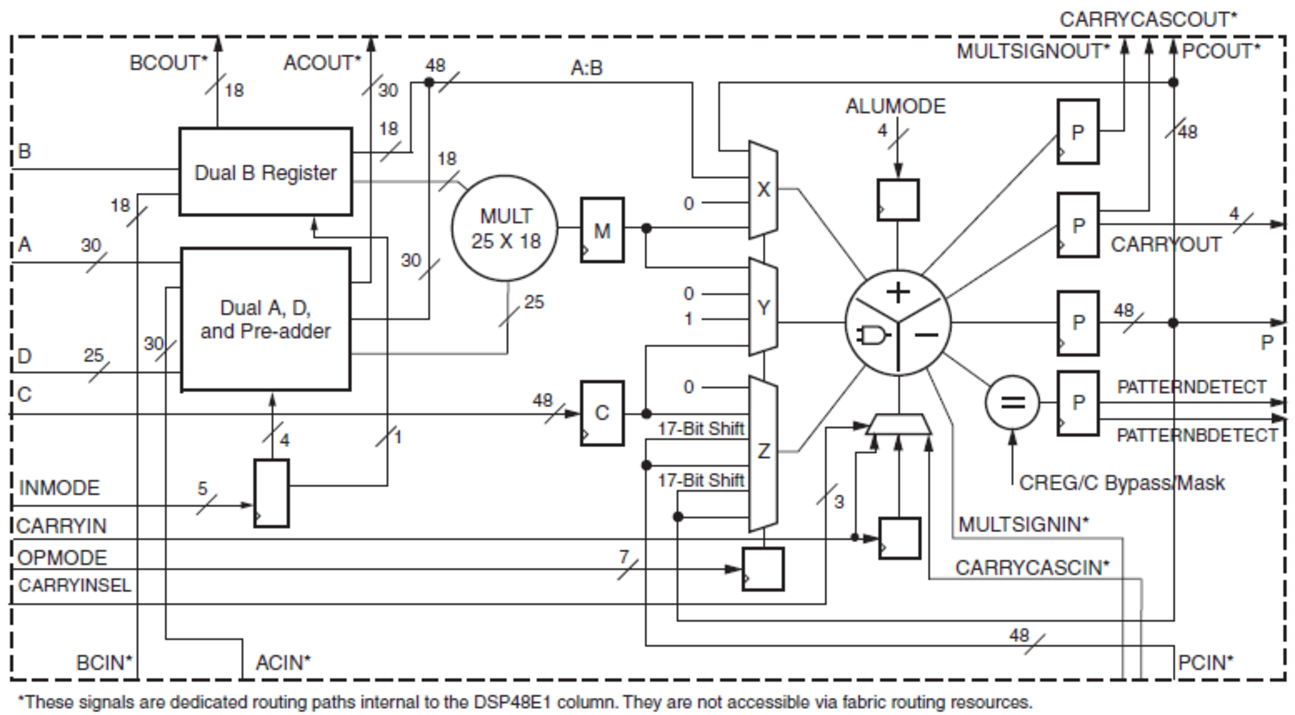
\includegraphics [width=0.9\columnwidth] {figures/DSP48E1.pdf} }
	\caption{Structure of DSP48E1 slice inside the Virtex-6 \cite{Xilinx2011}}
	\label{fig:DSP48E1}
\end{figure}

\begin{figure}
	\centerline{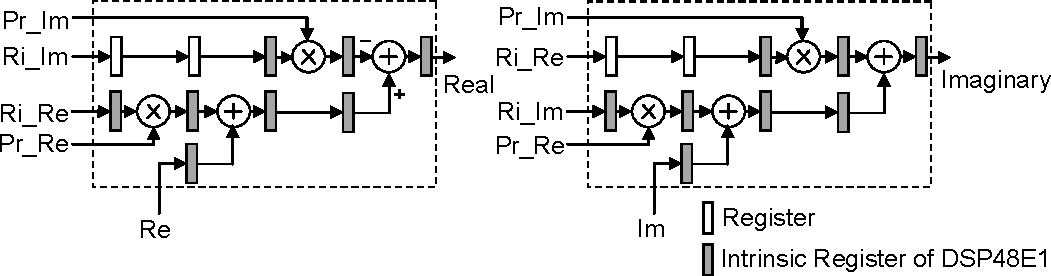
\includegraphics [width=0.9\columnwidth] {figures/Cmp_MultAdder.pdf} }
	\caption{Pipeline structure of the complex number multiply-add.}
	\label{fig:Cmp_MultAdder}
\end{figure}

\begin{figure}
	\centerline{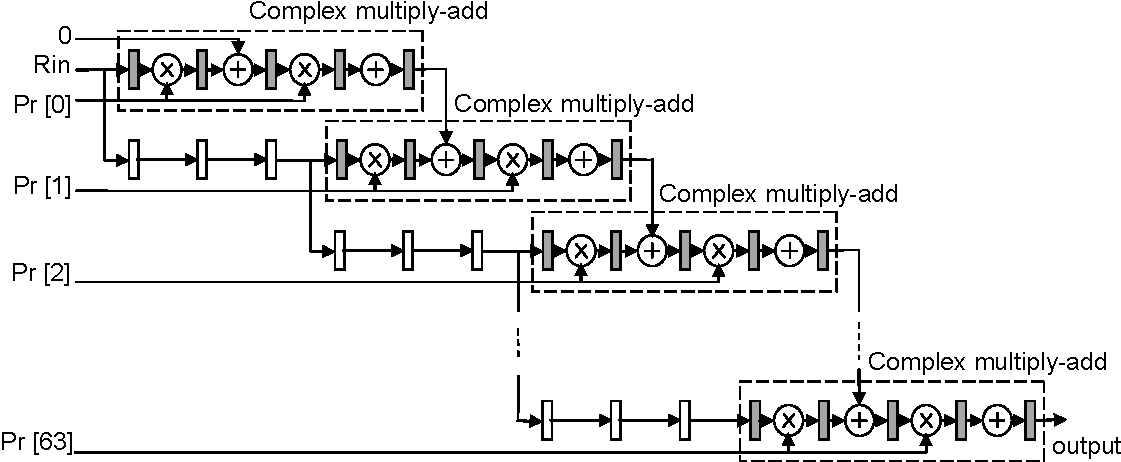
\includegraphics [width=0.9\columnwidth] {figures/DSP48pp_correlator.pdf} }
	\caption{Pipeline structure of correlator using DSP48E1 Slices.}
	\label{fig:DSP48pp_correlator}
\end{figure}

\begin{figure}
	\centerline{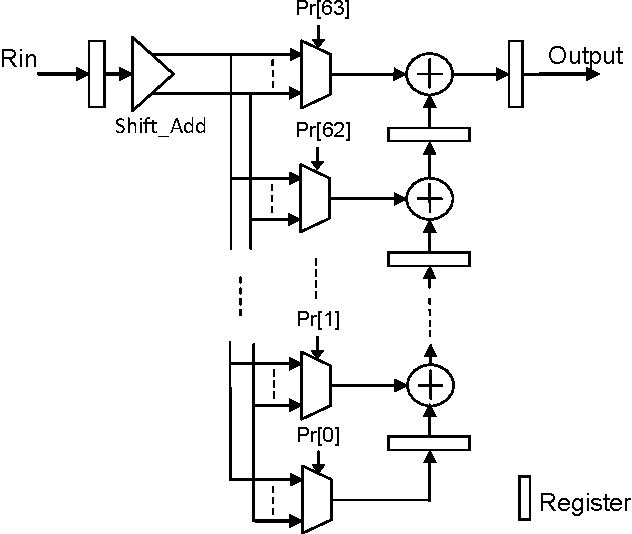
\includegraphics [width=0.7\columnwidth] {figures/ML_correlator.pdf} }
	\caption{Structure of multiplierless correlators.}
	\label{fig:ML_correlator}
\end{figure}

%---------------------------------------------------------------------------------
\subsection{Design of Multiplierless Correlator}

The principle of multiplierless correlators is to represent the coefficients and round them in the form of summed powers of two. 
Hence, a shift and add are performed instead of multiplying by coefficients. 
It is expected that multiplierless correlation is more efficient, but with embedded hard multipliers in modern FPGAs, it is unclear whether they should still be considered favourable. 
Furthermore, synchronisation accuracy must be considered.
To explore this, four alternative multiplierless correlators are implemented using four coefficient sets with an increasing degree of rounding, to compare the cost and performance and evaluate against multiplier-based correlators. 
The coefficient sets are found by quantising the 64 normalised preamble samples with quantisations of 1, 0.5, 0.25, and 0.125. 

The proposed structure for multiplierless correlators is shown in Fig. \ref{fig:ML_correlator}. 
This structure is based on the transpose-direct-form in Fig. \ref{fig:str_corr}. 
Instead of using multipliers to multiply input samples by coefficients, the $Shift\_Add$ block and multiplexers are used to perform the equivalent operation without an actual multiplication. 
But the  $Shift\_Add$ block, multilexers and value of $Pr[n]$ are different depending upon the quantised coefficient set being used.  
The $Shift\_Add$ block performs shift and add on received samples according to the degree of quantisation that is applied.  
To optimise resources in the case of small numbers of bit quantisation, one common $Shift\_Add$ block is used for all 64 coefficients instead of 64 separate $Shift\_Add$ blocks. 
This common $Shift\_Add$ block calculates all possible values for 64 coefficients.  
The multiplexers are used to select the corresponding values from $Shift\_Add$ to accumulate in order to generate the correlator output.
These are based on expressed coefficients $Pr[n]$ that are pre-computed based on quantizing the 64 preamble samples.
Since the $Pr[n]$ values are constants, after synthesising the design, the multiplexer is optimised as hard-wired logic, and the preamble cannot be changed.
To support different OFDM preambles, the $Pr[n]$ could be stored in a register, and a real multiplexer used instead of hard-wired logic.  
This results in increased resource utilisation but provides a more flexible solution. 

\subsection{Implementation Results}

The designs presented were synthesised and fully implemented using Xilinx ISE 13.2, targetting Xilinx Virtex-6 (V6) and Spartan-6 (S6) devices.  
The results of implementation are reported in terms of the number of occupied slices, DSP48E1s Slices and maximum frequency as summarised in Table \ref{tab:Imp_Rpt}. 

% Virtex-6 75T & Spartan-6 75T
\begin{table}[h]
	\centering
	\caption{Implementation Report}
	\label{tab:Imp_Rpt}
	\begin{tabular}{c|r|r|r|c|c}
        \hline \hline
    			Design  & \multicolumn{2}{|c|}{Occupied Slices} & DSP48E1s & \multicolumn{2}{|c}{Freq. (MHz)} \\
	\cline{2-6}			         & \makebox[1.2cm][c]{V6} & \makebox[1.2cm][c]{S6}& 	\makebox[1.2cm][c]{V6}	&  V6 & S6    \\
    	\hline
			DSPc 	& 742 		(6\%)  & -  			 & 256 (88\%) & 119 & -\\
			DSP\_pp &  1,110 	(9\%) & -  			 &  256 (88\%)& 398 & -\\
 			ML1 	&  661		(5\%) &	762 (6\%)	 &  0 (0\%)	& 309 & 174\\
			ML2 	&  983 	(8\%) &	1,071 (9\%) &  0 (0\%)	& 268 & 158\\
			ML3 	&  1,191 	(10\%) &	1,257 (10\%) &  0 (0\%)	& 234 & 136\\
			ML4 	&  1,496 	(12\%) &	1,517 (13\%) &  0 (0\%)	& 208 & 124\\   
    
    	\hline \hline  
    \end{tabular}	
\end{table}

$DSPc$, $DSP\_pp$ are correlator designs using DSP Slices, in non-pipelined and pipelined structures, respectively. 
$ML1$, $ML2$, $ML3$, $ML4$ are multiplierless correlators with coefficient quantisations of 1, 0.5, 0.25, 0.125, respectively.

Table \ref{tab:Imp_Rpt} reveals that the $DSP\_pp$ uses more logic slices due to its pipeline structure. 
The slices in DSP48E1 based designs are used for registers and route-thrus while the slices in the multiplierless designs are mostly used as logic. 
The number of slices used in the multiplierless designs increases as the coefficient quantisation becomes finer. 
The DSP48E1-based designs use 256 DSP Slices, 4 for each complex multiply plus 6-9\% of logic resources.
The multiplierless designs use only logic to compute the cross correlation with 64 complex coefficients. 
The total logic area is a small fraction of the whole device: around 5-12\% of total resources in the Virtex-6, and around 6-13\% of total resources in the equivalent Spartan-6.
While Spartan-6 devices do include DSP Slices, their number is insufficient to implement the full 64 sample complex cross correlation.
This shows an ideal scenario where multiplierless correlation makes sense, and hence serves as a motivation for this study.

The maximum frequencies, reported after place and route, decrease for multiplierless designs according to the degree of coefficient quantisation. 
Meanwhile the non-pipelined DSP48E1 design is slower than the multiplierless designs. 
However, the pipelined DSP48E1 design can achieve higher frequency.

A post-place-and-route simulation in ModelSim was used to estimate the power consumption of the system using the Xilinx XPower tool. 
Table \ref{tab:PWR} shows the power dissipation of the designs running at 50{\thinspace}MHz. 
The DSP48E1-based correlators consume more power than the multiplierless correlators, but this is due primarily to increased dynamic power when using the DSP48E1s on the Virtex-6. 
The dynamic power of the non-pipelined DSP48E1-based correlator $DSP\_Cor$ is greatest at 846{\thinspace}mW, but pipelining reduces this by a factor of more than 2.5 times, due to reduced switching activity between the multiplier and adder.  
The dynamic power of the multiplierless designs increases from 133{\thinspace}mW to 203{\thinspace}mW on Virtex-6 and from 149{\thinspace}mW to 294{\thinspace}mW on Spartan-6 as finer coefficient quantisation is used. 
It is important to note that the quiescent power of the Spartan-6 is much lower by design. 
Hence, we can see that using this multiplierless technique allows us to implement synchronisation on a Spartan-6 device, where a multiplier-based design is not possible, saving significant power and sacrificing little in terms of accuracy.

 % Virtex-6 75T  &  Spartan-6 75T
\begin{table}[h]
	\centering
	\caption{Power Consumption at 50MHz.}
	\label{tab:PWR}
	\begin{tabular}{c|c|c|c|c|c|c}
        \hline \hline
    			Correlators  & \multicolumn{2}{|c|}{Quiescent(mW)} &  \multicolumn{2}{|c|}{Dynamic(mW) }& \multicolumn{2}{|c}{Total(mW)} \\
	\cline{2-7}			& V-6 & S-6 & V-6 & S-6 & V-6 & S-6\\
	\hline
			DSP\_Cor		&  1312 &  -  	 & 846 & -	& 2158 &-\\
			DSP\_pp\_Cor 	& 1300  &  -   & 328 & - 	& 1628 & -\\
 			ML1\_Cor 		& 1296  & 67 & 133 & 149	& 1429 & 216\\
			ML2\_Cor 		& 1296  & 68 & 160 & 197	& 1456 & 265\\	
			ML3\_Cor 		& 1297  & 70 & 182 & 239	& 1479 & 309\\
			ML4\_Cor 		& 1297  & 71 & 203 & 294    & 1500 & 365\\   
    
    	\hline \hline  
    \end{tabular}
\end{table}


\begin{figure}
	\centerline{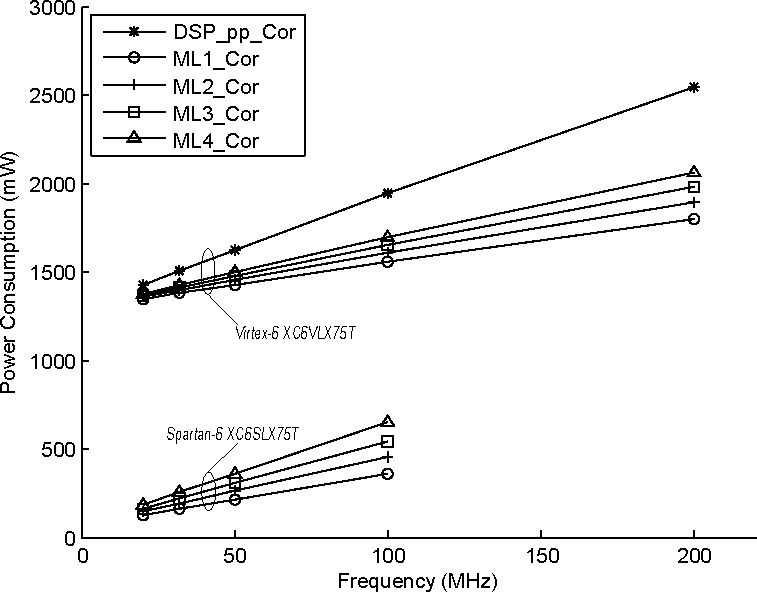
\includegraphics [width=0.9\columnwidth] {figures/Plot_PWR.pdf} }
	\caption{Power consumption of designs.}
	\label{fig:Plot_PWR}
\end{figure}

We also investigated how total power consumption varies with frequency, as shown in Fig. \ref{fig:Plot_PWR}.
As frequency increases, the finer quantisations and DSP48E1-based designs begin to consume proportionally more power.
Overall, multiplierless designs on the Spartan-6 consume 75\% to 85\% less power than the same designs on the Virtex-6, and a 0.25 quantisation design on the Spartan-6 consumes 81\% to 85\% less power then the DSP48E1-based design on a Virtex-6.

The \emph{DPS\_Cor} implementation represents how a ``blind'' design would be mapped. Our architecture-aware designs show significantly better performance, reduced area, and reduced power consumption.

%---------------------------------------------------------------------------------
\section{Simulation and discussion}
%---------------------------------------------------------------------------------
In order to validate our designs at the application level, we simulate them using ModelSim with an IEEE802.16 OFDM frame created using MATLAB, including the preamble symbols, data symbols and effects of an AWGN channel. 
Cross-correlation results using the correlator designs are compared to corresponding results in MATLAB to verify the correctness of implementation. 
To evaluate the accuracy of timing synchronisation acheivable by these designs, the correlation outputs are plotted in Fig. \ref{fig:Plot_XCR} for random data frames at 10{\thinspace}dB SNR. 
The output of each correlator is slightly different because of rounding, but the timing synchronisation depends upon the location of the peaks being at the  position of the preamble.
All the correlator designs achieve this most of the time, as shown at indices 34 and 98 for the CP samples and the first preamble samples respectively, for a single frame. 
 
\begin{figure}
	\centerline{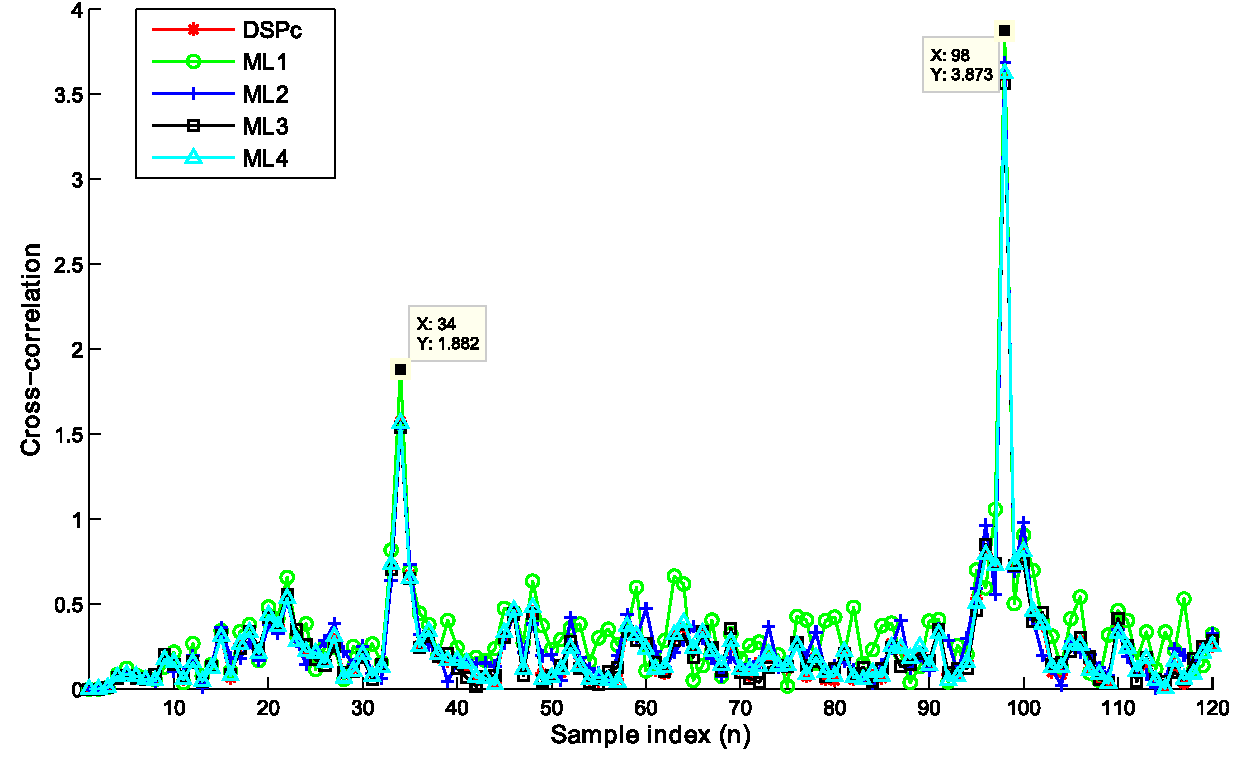
\includegraphics [width=0.9\columnwidth] {figures/Plot_XCR.pdf} }
	\caption{Correlator output with SNR = 10dB.}
	\label{fig:Plot_XCR}
\end{figure}

In order to evaluate the synchronisation accuracy of these approaches, we simulate 10,000 correlation operations in an AWGN channel with a detection strategy as follows. 
First, find the first peak, $P1$, over 64 samples. 
Next, find the second peak, $P2$, in the next 64 samples from the first peak and compute average value, $avg$, of the samples between two peaks. 
If  $( P1 - avg ) \le  0.75 * ( P2 - avg )$, the start of frame is detected and the correctness of the position can be checked. 
It should be noted that in all cases, the peaks were known to be located within the two search regions and that the detection strategies described above are compatible with those of other authors such as \cite{Kishore2006} and \cite{Yip2003}. 
Fig. \ref{fig:Plot_NFail} plots the results in terms of failure rate against AWGN SNR and show that the designs are able to accurately detect the start of frame even in low SNR conditions. 
The failure rate of $ML1\_Cor$ is the highest, as expected, due to the coarse quantisation.
For SNRs above 4{\thinspace}dB, the failure rates of $ML2\_Cor$, $ML3\_Cor$,  $ML4\_Cor$ and $DSP\_Cor$ differ less than 0.05\% from each other.
This suggests that sacrificing accuracy by using multiplierless cross-correlation is feasible and has negligible impact on synchronisation accuracy.
Combined with the results in the previous section, we can be confident that low-power FPGAs, such as the Spartan-6, with insufficient resources for multiplier-based synchronisation correlation, are still feasible for implementing robust OFDM receivers.

\begin{figure}
	\centerline{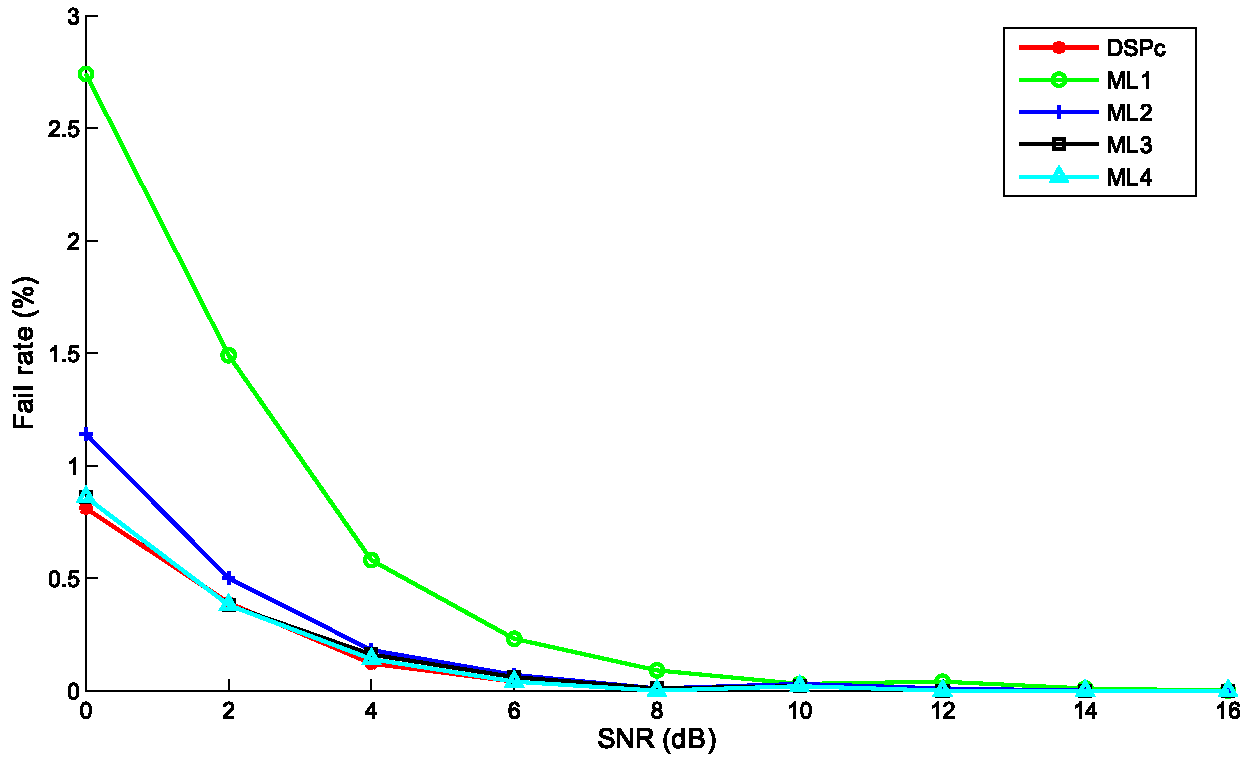
\includegraphics [width=0.85\columnwidth] {figures/Plot_NFail.pdf} }
	\caption{Detection failure rate.}
	\label{fig:Plot_NFail}
\end{figure}

%---------------------------------------------------------------------------------
\section{Summary}
%---------------------------------------------------------------------------------
The DSP48E1 Slices on modern Virtex-6 FPGA devices seem to offer the ideal resource for implementing correlation-based frame synchronisers.
However, as we have discovered, in the context of synchronisation for IEEE802.16 OFDM systems, simplified multiplierless designs offer comparable synchornisation performance. 
While the DSP48E1-based correlators can obtain higher clock speeds, this is only possible through a detailed pipelined design.
Furthermore, their power consumption and resource usage is considerably greater.
Since low-power, low-cost devices such as the Xilinx Spartan-6 do not include sufficient DSP Slices, this suggests adopting multiplierless designs for low-power implementations.
We have shown that while very low quantisation resolution does impact synchronisation performance, with a step size of just 0.5, synchronisation accuracy is on par with multiplier-based correlation. 
Multiplierless correlation on a Spartan-6 can save over 85\% power compared to  a DSP Slice design on a Virtex-6 FPGA.

This work has been submitted as a journal paper to  IEEE transactions on Very Large Scale Integration (VLSI) systems.
\chapter{Multiplierless Correlator Design for low-power systems}
\label{chap:multiplierlesscorrelator}
%%---------------------------------------------------------------------------------
\chapter{Method for OFDM Timing Synchronisation}
\label{chap:Synchronisation}
%---------------------------------------------------------------------------------

%---------------------------------------------------------------------------------
\section{Introduction}
%---------------------------------------------------------------------------------
OFDM performance is sensitive to receiver synchronisation \cite{Hanzo2006}.
Frequency offset causes inter-subcarrier interference, and errors in timing synchronisation can lead to inter-symbol interference.
Therefore, accurate synchronisation is critical to the performance of OFDM systems.
This section summarises conventional synchronisation methods used with OFDM, discussing their merits and drawbacks, before the following sections present a new and efficient method that is robust to large frequency offset, obtains accurate  and robust synchronisation and requires relatively low computational complexity. In particular, it is designed to be suitable for hardware implementation on reconfigurable systems.

The method presented in this chapter has also been discussed in:
\begin{itemize}
\item T. H. Pham, I. V. McLoughlin, and S. A. Fahmy, ``Robust and Efficient OFDM Synchronisation for FPGA-Based Radios,'' in \textit{Circuits, Systems, and Signal Processing, vol. 33, no. 8, pp. 2475 - 2493, Aug. 2014, Springer}~\cite{Pham2014}.
\end{itemize}

%---------------------------------------------------------------------------------
\section{Related Work}
%---------------------------------------------------------------------------------
Autocorrelation-based methods are commonly chosen for implementing synchronisation because of their low computational complexity. In \cite{Schmidl1997}, timing metrics are defined as follows, beginning with the normalised power measure \emph{M[d]}:

\begin{center}
\begin{equation}
\label{MMetric}
M[d] = \frac{|P[d]|^2} {(R[d])^2},
\end{equation}
\end{center}

where $d$ denotes a time index corresponding to the first sample in a search space comprising $2L$ samples of received signal $r$. The power measure \emph{R}, which represents the energy of the second half of the receiver search window, is defined as:

\begin{center}
\begin{equation}
\label{RMetric}
R[d] =\sum_{m =0}^{L-1}   |r[d+m+L]|^2,
\end{equation}
\end{center}

and the normalisation parameter \emph{P} computes the correlation between two periodic halves in the search window as:

\begin{center}
\begin{equation}
\label{PMetric}
P[d] =\sum_{m =0}^{L-1}    (r^{*}[d+m] r[d+m+L] ),
\end{equation}
\end{center}

%where superscript \textquotedblleft$*$\textquotedblright  denotes complex conjugation.

The metric \emph{M[d]} is illustrated for a typical channel in Fig.~\ref{fig:M1-10dB}, where it can be seen to form a distinct plateau in the region when the preamble is presented within a received window.
Clearly, \emph{M[d]} accurately detects the preamble, however the nature of the plateau having a flat top presents an uncertainty in terms of exact positioning, and hence reduced accuracy in determining the exact start of the frame, compared to a metric which peaks.

\begin{figure}
	\centerline{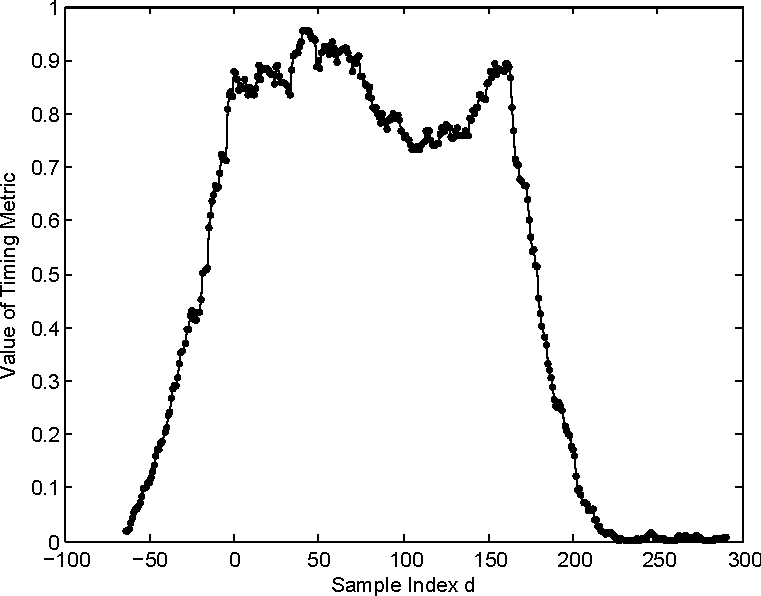
\includegraphics [width=0.8\columnwidth] {figures/M1_10dB.pdf} }
	\caption{The timing metric in \cite{Schmidl1997} applied to the IEEE~802.16-2009 preamble in an AWGN channel (SNR = 10dB)}
	\label{fig:M1-10dB}
\end{figure}

In order to improve the accuracy of synchronisation, a scheme is often used as in \cite{Schwoerer2002,Manavi2004,Guffey2007,Huang2010,Recio2010} based on combining the above metric for detecting the frame, estimated coarse STO and fractional CFO, and additional cross-correlation operations for computing fine STO and integer CFO as we will explore below.

%---------------------------------------------------------------------------------
\subsection{Coarse STO and Fractional CFO Estimation}
%---------------------------------------------------------------------------------

First, the plateau of the \emph{M[d]} metric is used to detect a frame start and estimate coarse STO by comparing the magnitude of \emph{M[d]} to a given threshold. After this, the CFO is estimated using the \emph{P} metric in (\ref{PMetric}).
We now assume that we are receiving a signal \emph{s[d]} which has a normalised carrier frequency offset $\xi$ with respect to \emph{r[d]}:
\begin{center}
\begin{equation}
\label{freoffsignal}
s[d] =  e^{j2\pi\xi \frac{d}{N}}*r[d].
\end{equation}
\end{center}
where \emph{N} is the numbers of subcarriers of the OFDM symbol. At the plateau of \emph{M[d]}, the received samples in the window will be periodic:
\begin{center}
\begin{equation}
\label{signalperiodic}
r[d] =  r[d+L].
\end{equation}
\end{center}

Substituting (\ref{freoffsignal}) and  (\ref{signalperiodic}) in (\ref{PMetric}) we find that

\begin{eqnarray}
\label{PMetricfreoffset}
P[d] &=& \sum_{m =0}^{L-1}  (s^{*}[d+m] s[d+m+L] ) \nonumber \\
 &=& e^{j2\pi \xi \frac{L}{N}} \sum_{m =0}^{L-1}  |r[d+m]|^2
\end{eqnarray}
The CFO can be determined as follows;
\begin{equation}
\label{fractionalCFO}
\xi = \frac{\angle P[d] + 2\pi z}{2\pi \frac{L}{N}}
\end{equation}
where  $\angle P[d]$ is the angle of \emph{P[d]} within the range -$\pi$ to $\pi$.
The CFO consists of 2 parts: the fractional part, $\hat{\lambda} = \frac{\angle P[d]}{2\pi \frac{L}{N}}$, can be estimated replied on $\angle P[d]$ and the integer part (IFO) is represented by an integer \emph{z}, $\hat{\epsilon} = \frac{z N}{L}$.
The fractional CFO estimation has a range limitation as follows:
\begin{eqnarray}
\label{fractionalCFOlimitation}
 -\frac{N}{2L} & <  \hat{\lambda}   < & \frac{N}{2L}
\end{eqnarray}

Clearly, the range over which fractional CFO can be estimated may be increased by decreasing the length of period \emph{L}.
However, because of the influence of channel noise, a smaller \emph{L} would also degrade the accuracy of estimation of the fractional CFO $\hat{\lambda}$.
In the case of the IEEE~802.16-2009 preamble~\cite{IEEE80216}, the number of subcarriers \emph{N} and length of period \emph{L} are commonly chosen to be 512 and 64 samples respectively \cite{Kim2008}.
Hence the fractional CFO estimation range is limited to within -2 to +2 subcarrier spacings. Meanwhile, the value of IFO parts $\hat{\epsilon}$ is estimated as an integer multiple of 4.

The method outlined above is fast and robust for estimating coarse STO and fractional CFO.
However it has some drawbacks.
First, the coarse STO is estimated by comparing the metric to a threshold.
It is not certain that the samples for estimating the fractional CFO are within the plateau of \emph{M[d]} in which the received samples in the window will be periodic.
This degrades the performance of fractional CFO estimation.
Second, the CFO estimation can only be performed correctly in the limited range of the fractional CFO shown in (\ref{fractionalCFOlimitation}).
If the actual CFO lies outside this range, it is necessary to estimate the integer CFO separately.

%---------------------------------------------------------------------------------
\subsection{Fractional CFO Compensation}
%---------------------------------------------------------------------------------

Fine STO estimation, accomplished using cross-correlation, is sensitive to CFO.
Thus the estimated fractional CFO must first be used for frequency offset compensation.
This is done by phase de-rotating the received samples in the time domain:

\begin{eqnarray}
\label{comfreoffsignal}
\widehat{r[d]} =  e^{-j2\pi\xi \frac{d'}{N}}*s[d];  & d' = d + \mathit{t_{off}}.
\end{eqnarray}

$\widehat{r[d]}$ and \emph{s[d]} are the compensated samples and frequency offset samples, respectively. \emph{d'} is the coarse estimated timing index that differs from the correct timing index $\mathit{t_{off}}$ samples.
Substituting (\ref{freoffsignal}) in (\ref{comfreoffsignal}), we get:

\begin{eqnarray}
\label{phaseerror}
\widehat{r[d]} &=&  e^{-j2\pi\xi \frac{(d+t_{off})}{N}}*e^{j2\pi\xi \frac{d}{N}}*r[d] \nonumber \\
&=& e^{-j2\pi\xi \frac{t_{off}}{N}}*r[d].
\end{eqnarray}

When compensating the fractional CFO, the fine STO has still not been estimated. This results in a common phase error within the coarse CFO compensated samples as shown in (\ref{phaseerror}).

%---------------------------------------------------------------------------------
\subsection{Fine STO Estimation}
%---------------------------------------------------------------------------------

The purpose of timing synchronisation is to find the correct starting point for receiver demodulation.
This starting point will generally mark the beginning of a discrete Fourier transform (DFT) window.
Coarse time synchronisation is commonly based on auto-correlation as mentioned above, leading to relatively simple hardware implementation.
However, with purely coarse STO, it is almost impossible to achieve sufficient accuracy to correctly detect the starting point.
Thus,  fine STO estimation is necessary to refine the accuracy of timing synchronisation.
To obtain more accurate fine STO estimation, cross-correlation is usually performed between the received samples and known transmitted preamble.
The peak cross-correlation occurs when the received samples match the known preamble.
Fine STO can thus be found by locating this peak within a search window.
In order to reduce the overhead of cross-correlation, a sign bit multiplier can be used instead of a real multiplier to calculate cross-correlation. However, this is much more sensitive to CFO in practice \cite{Schwoerer2002}. Some researchers employ enhanced methods based on cross-correlation for the time synchronisation.
For example, Kishore and Reddy \cite{Kishore2006} presented an algorithm using cross-correlation between the known transmitted and received preamble symbols.
The timing metrics for synchronisation using this method perform the normalised \emph{M[d]} calculation, and use the same denominator \emph{R} as in (\ref{MMetric}) and (\ref{RMetric}), however they refine the numerator \emph{P} as follows;
\begin{center}
\begin{equation}
\label{PKishore}
P[d] =\sum_{m =0}^{L-1}    (r[d+m] a[m])^{*} (r[d+m+L] a[m]),
\end{equation}
\end{center}
where $d$ again denotes the time index corresponding to the first sample in a window of \emph{2L} samples of received signal $r$ and superscript \textquotedblleft$*$\textquotedblright again denotes complex conjugation. In (\ref{PKishore}) the samples $a$ are now the known, transmitted, time domain preamble samples.

The cross correlation now produces distinct peaks at the times when received samples match the known transmitted samples of the preamble. Fig.~\ref{fig:M2-10dB} illustrates this by plotting \emph{M} versus the sample index $d$ for an example channel in AWGN with SNR~=~10{\thinspace}dB.
A frame is detected when \emph{M} crosses a threshold and the start of frame is found by searching the peaks of \emph{M}.
This can accurately determine the start of frame even at low SNRs.
Moreover, this method is robust to large CFO for time synchronisation.
Simulations \cite{Kishore2006} show that time synchronisation can be performed effectively with CFO~=~10.5 subcarrier spacings.
However, the cross-correlation operation requires complex computation.
Although the complexity of cross-correlation can be reduced using multiplierless correlation \cite{Yip2003}, the multiplierless correlator degrades the precision of metric \emph{P}, used for estimating frequency offset.
In general, this method is appropriate for time synchronisation but requires significant hardware resources for implementing the cross-correlation.

\begin{figure}
	\centerline{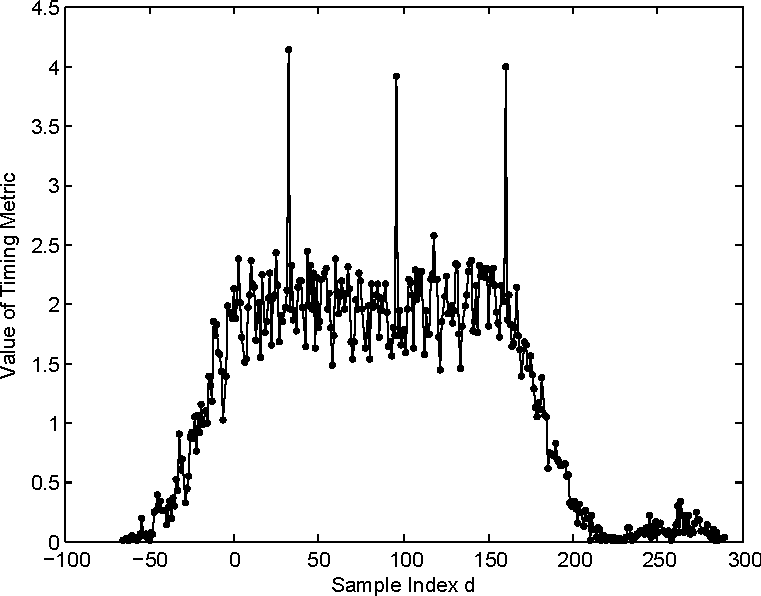
\includegraphics [width=0.8\columnwidth] {figures/M2_10dB.pdf} }
	\caption{The timing metric in \cite{Kishore2006} applied to the IEEE~802.16 preamble in an AWGN channel (SNR = 10dB)}
	\label{fig:M2-10dB}
\end{figure}

%---------------------------------------------------------------------------------
\section{Proposed Fractional CFO Estimation and Synchronisation}
%---------------------------------------------------------------------------------

Considering the limitations of previous work, we propose new timing metrics to take advantage of preamble characteristics such as period and energy distribution.
Again, the proposed method is illustrated for the specific case of the IEEE~802.16-2009 preamble, as shown in Fig.\ref{fig:SyncFlow}.

Firstly, we define the autocorrelation between the two halves of the receiver window for normalisation purposes;

\begin{equation}
\label{ProposedP}
P'[d] =\sum_{m =0}^{C-1}    (r^{*}[d+m] r[d+m+L] )
\end{equation}

where $d$ denotes a time index of received signal $r$ that now corresponds to the first sample in a window of \emph{L+C} samples of received signal, \emph{L} being the length of preamble period (64 for the IEEE802.16 preamble) and \emph{C} being the length of received samples for estimation, respectively.

Next, a power measure, \emph{R'} is proposed which takes account of both received and transmitted symbol power;

\begin{equation}
\label{ProposedR}
R'[d] =\sum_{m =0}^{C-1}   |r[d+m+L]|^2  |a[m]|^2
\end{equation}


\begin{figure}
\centering
	\begin{tikzpicture}
	\begin{axis}[ xlabel= Sample index d, ylabel= Value of Timing Metric, legend columns=3,	legend style={at={(0.5,1.02)}, anchor=south, cells={anchor=west}, draw=none}, x post scale=1.4]
		\addplot+[black, style={densely dashed, color=violet, thick}, every mark/.append style={mark=none}]  table [x index=0, y index=1] {./Dat/Pp_Rp.dat};
		\addlegendentry{P' Metric};
		\addplot+[black, style={solid, color=red, thick}, every mark/.append style={mark=none}]	 table [x index=0, y index=2] {./DAT/Pp_Rp.dat};
		\addlegendentry{R' Metric};
	\end{axis}
	\end{tikzpicture}
	\caption{Proposed timing metrics applied to the IEEE~802.16 preamble in AWGN (SNR = 10{\thinspace}dB, CFO = 10.5).}
	\label{fig:ProposedMetric-10dB}
\end{figure}


In common with the metric developed by Schmidl and Cox \cite{Schmidl1997}, our proposed \emph{P'[d]} detects the periodic characteristic of the preamble and can thus be used for estimating fractional CFO.
\emph{P'} forms a plateau as evident in Fig.\ref{fig:ProposedMetric-10dB} when the preamble is present within the receiver window.
\emph{R'} is then used to find the starting point of the preamble based on its energy distribution.
\emph{R'} causes peaks shown in Fig.\ref{fig:ProposedMetric-10dB} at the point where the energy distribution of the received samples matches that of the transmitted preamble.
Since the \emph{R'} metric that is used to estimate time synchronisation is computed on the square of the amplitude of received samples, the time synchronisation is insensitive to the CFO that effects the phase of the received samples.
Moreover, computing on amplitude squared, a real number, requires less resources than using complex numbers as in alternative approaches such as \cite{Kishore2006}.
In addition, the time synchronisation is performed based on the peak value of \emph{R'} rather than its absolute value.
Therefore, \emph{R'} is a good candidate for implementation using a multiplierless correlator to reduce computational complexity.
\begin{figure}
	\centerline{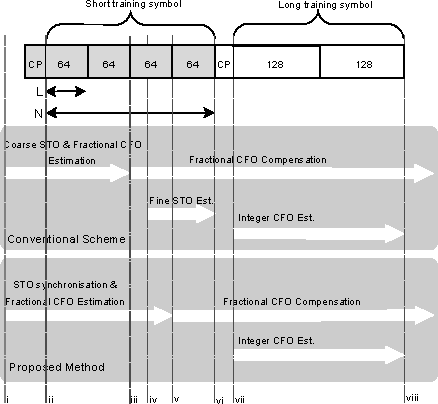
\includegraphics [width=1\columnwidth] {figures/SynFlow_IVMannotated.pdf}}
	\caption{The synchronisation flow according to the received samples within the preamble showing its packet format above the conventional synchronisation scheme flow (middle), and proposed scheme (bottom). With the packet timing illustrated above.}
	\label{fig:SyncFlow}
\end{figure}
Fig.\ref{fig:SyncFlow} illustrates the flow of the proposed synchronisation method according to the received samples of the preamble, compared to that of the conventional scheme.
As can be seen in the conventional scheme, the coarse STO and fractional CFO estimation are performed in the two first periods of the short training symbol from (i) to (iii), and then the estimated fractional CFO is used for compensation.
The fine STO is estimated in the last period of the short training symbol from (iv) to (vi), and integer CFO should be computed in the long training symbol from (vii) to (viii).
By contrast, the proposed method performs STO synchronisation and fractional CFO estimation in the three first periods of the short training symbol from (i) to (iv), and the start of frame will be detected at (ii).
Then, the fractional CFO compensation is computed, and integer CFO estimation is performed in the long training symbol from (vii) to (viii).

The method used for synchronisation based upon these metrics is described in the following sub-sections.

\subsection{Frame Synchronisation and Fractional CFO Estimation}

First, frame detection is performed by comparing the metric \emph{P'} to \emph{R'} with a threshold \emph{thr} as shown in (\ref{framedetection})
\begin{equation}
\label{framedetection}
|P'[d]| > thr * R'[d].
\end{equation}

%The threshold is different for each channel and needs to be determined empirically by simulation (in common with other systems such as \cite{Kishore2006}).
Fig.\ref{fig:TimeSyn_thr_AWGN} shows the performance of the frame synchronisation in the given channel for different threshold values.
With each threshold value, 1000 frame detections are simulated.
\begin{figure}
	\centerline{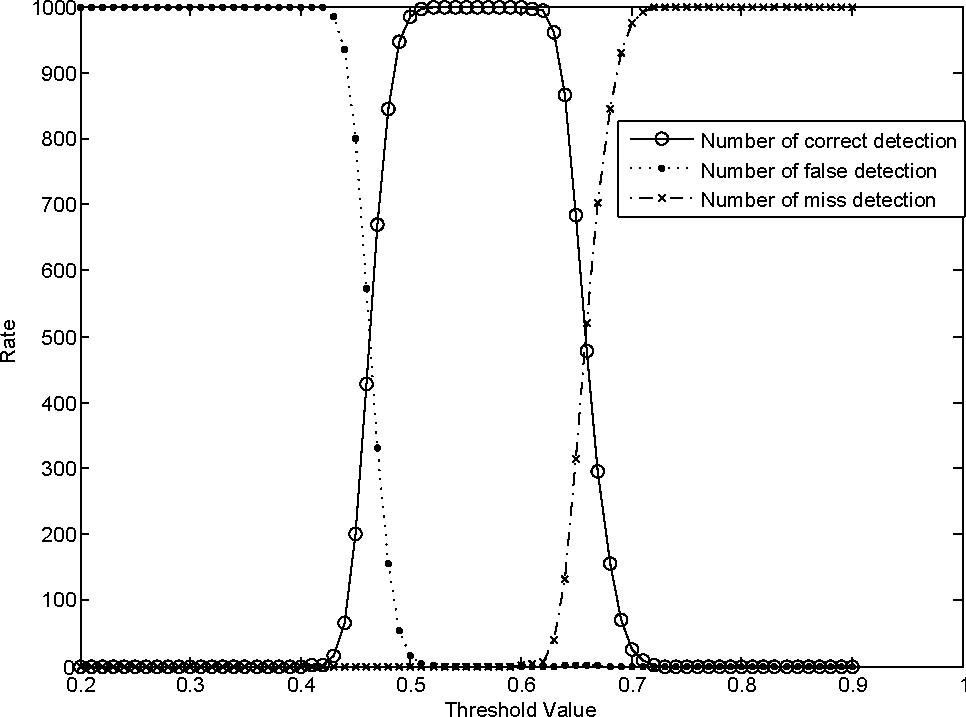
\includegraphics [width=0.9\columnwidth] {figures/ThresholdEffect.pdf}}
	\caption{Performance of the frame synchronisation method versus the selection threshold for an AWGN channel (with SNR =10dB).}
	\label{fig:TimeSyn_thr_AWGN}
\end{figure}
The number of correct detections indicates how often the time synchronisation has been found correctly at the start of the frame, while the number of false detections indicate that the time synchronisation gets the wrong start of the frame.
Otherwise, the frame is not detected (i.e. $|P'[d]|$ can be not greater than $thr * R'[d]$), and a miss detection is declared.
From the results plotted,  the optimum value can be seen to be around 0.55.
If the threshold is too small, noise may cause a failure of detection.
On the other hand, when the threshold is large, the frame detection may be missed if the noise reduces the amplitude of the timing metric, which consequentially does not cross the threshold.
The threshold values depend on the operating channel and are determined empirically by simulation (in common with other systems such as in [36]). Assuming the set of possible channels is known, the thresholds for these channels can be pre-determined by simulation. The performance of synchronisation is evaluated with increased thresholds for a given channel model. The threshold value corresponding to the best performance is selected for the channel model. The determined threshold values are stored in a look-up table. Based upon current channel model and conditions, a threshold is selected from the look-up table.



After a frame is detected, the starting point of the short preamble is found by searching for the peaks in \emph{R'[d]}.
As can be seen in Fig. \ref{fig:ProposedMetric-10dB}, two peaks in \emph{R'[d]} will bracket the transition to the plateau in \emph{P'[d]} shown at sample indices of -31 and 33, respectively.
The second peak is used as the starting point for the DFT window.
This is accomplished for the maximum values of $R'[d] + R'[d - L]$ over the next \emph{L} samples after frame detection.
Second, the fractional CFO estimation is presented in (\ref{proposedfractionalCFO}) based on the \emph{P'[d]} metric similarly to other work such as \cite{Schmidl1997,Schwoerer2002,Manavi2004,Guffey2007,Huang2010,Recio2010};

\begin{equation}
\label{proposedfractionalCFO}
\hat{\lambda} = \frac{\angle P'[d]}{2\pi \frac{L}{N}}
\end{equation}
where $\hat{\lambda}$ is the estimated fractional CFO, $\angle P'[d]$ denotes the angle of \emph{P'[d]} and \emph{N} is the number of subcarriers.
In this proposed method, the fractional CFO is estimated at the starting point of the preamble to guarantee that the correct angle of \emph{P'[d]} is taken for estimation. Using the conventional techniques, the inherent uncertainty in the coarse STO does not allow this to be achieved in practice.
Thus, the estimated fractional CFO in the proposed method will, on average, tend to be more accurate.
In addition, this method separates the length of preamble period \emph{L} and the length of received samples for estimation \emph{C}, and because of that \emph{L} can be small to extend the range of fractional CFO, and \emph{C} can be longer to increase the robustness to channel noise. For the IEEE~802.16 preamble, \emph{C} is set equal to \emph{2L} to improve the overall precision of synchronisation.

\subsection{Fractional CFO Compensation}

Compensating the fractional CFO is performed in the traditional way by phase de-rotating the received samples in the time domain;

\begin{eqnarray}
\label{proposedcomfreoffsignal}
\widehat{r[d]} &=&  e^{-j2\pi\Delta f_{c}dT_{s}}*s[d]. \nonumber \\
&=&  e^{-j2\pi\xi \frac{d}{N}}*e^{j2\pi\xi \frac{d}{N}}*r[d] \nonumber \\
&=& r[d].
\end{eqnarray}
However, in this proposed method, the frame synchronisation is achieved before performing fractional CFO compensation, therefore, $t_{off}$ is removed, and thus, the common phase errors caused by fractional CFO compensation are missing.
The compensated received samples are then demodulated using the DFT to obtain the received symbols in the frequency domain.

%---------------------------------------------------------------------------------
\subsection{Simulation Results and Discussion}
%---------------------------------------------------------------------------------
In this section, we will evaluate the performance of the proposed synchronisation method, applied to the IEEE~802.16-2009 downlink preamble, in MATLAB under both AWGN channels as well as the more realistic SUI channels that are widely used in the research literature \cite{Kishore2006,Kim2008}.

The Stanford University Interim (SUI) channel model~\cite{V.ErcegJuly2003} is used to simulate a frequency selective channel and takes into account  many wireless channel effects including delay spread, Doppler spread, phase noise, and channel interference.
In addition, the value of metrics computed in MATLAB are later verified with corresponding values from the FPGA simulation, to ensure practical functional equivalence.

In total, 100,000 OFDM frames, preceded by noise with randomly seeded AWGN and followed by preamble and data symbols, are used to evaluate synchronisation performance for each method.
The proposed method is compared to the state of the art method, in terms of accuracy of both time synchronisation and fractional CFO estimation.
The performance of STO estimation is measured in terms of failure rate (\%), and the accuracy of CFO estimation is evaluated in terms of mean square error (MSE).
We separately evaluate the robustness of time synchronisation against large CFO for each method.
Three versions of the proposed approach are constructed by varying the length, \emph{C}, of received samples for estimation based on (\ref{ProposedP}). These are investigated to determine the tradeoff between accuracy and computational cost, with \emph{C} defined as follows in each case:
\begin{itemize}
\item \textit{Prop 1}: $C=L$
\item \textit{Prop 2}: $C=2L$
\item \textit{Prop 3}: $C=3L$
\end{itemize}
These are compared to the state of the art method (denoted as \textit{SoA}) \cite{Liu2009,Recio2010}, and the method of Kishore and Reddy \cite{Kishore2006} (denoted as \textit{K\&R}) for a number of evaluation scenarios.
First, the performance of each method is found for AWGN channels beginning with CFO = 0.5, then AWGN channels with CFO varying from -10 to +10 times carrier spacing, then SUI1, and finally SUI2 channels.

		\subsubsection{Performance in AWGN}
\begin{figure}[h]
\centering
    	\begin{tikzpicture}
	\begin{semilogyaxis}[ xlabel=SNR(dB), ylabel=Fail rate of frame synchronisation (\%), legend columns=3,	legend style={at={(0.5,1.02)}, anchor=south, cells={anchor=west}, draw=none},
						 xmax=16, ymin=0.001, ymax=100, x post scale=1.4]
		\addplot+[style={dashed, thick},every mark/.append style={mark=square, style=solid}] table [x index=0, y index=4] {./Dat/FailRate_AWGN.dat};
		\addlegendentry{ \textit{Prop3}};
		\addplot+[style={solid, thick},every mark/.append style={mark=diamond*, style=solid}] table [x index=0, y index=3] {./Dat/FailRate_AWGN.dat};
		\addlegendentry{ \textit{Prop2}};
		\addplot+[style={dotted, thick},every mark/.append style={mark=triangle, style=solid}] table [x index=0, y index=2] {./Dat/FailRate_AWGN.dat};
		\addlegendentry{ \textit{Prop1}};
		\addplot+[black, style={solid, thick},every mark/.append style={mark=*, style=solid}] table [x index=0, y index=1] {./Dat/FailRate_AWGN.dat};
		\addlegendentry{ \textit{SoA}};
		\addplot+[style={dashed, thick},every mark/.append style={mark=o, style=solid}]  table [x index=0, y index=9] {./Dat/FailRate_AWGN.dat};
		\addlegendentry{ \textit{K\&R}};
	\end{semilogyaxis}
	\end{tikzpicture}
\caption{Performance of time synchronisation in AWGN channels with a frequency offset of 0.5 subcarrier spacings.}
\label{fig:STO_AWGN}
\end{figure}

\begin{figure}[h]
\centering
    	\begin{tikzpicture}
	\begin{semilogyaxis}[ xlabel=SNR(dB), ylabel=MSE of Fractional CFO,  legend columns=3, legend style={at={(0.5,1.02)}, anchor=south, cells={anchor=west}, draw=none}, x post scale=1.4]
		\addplot+[style={dashed, thick},every mark/.append style={mark=square, style=solid}] table [x index=0, y index=4] {./Dat/Fest_AWGN.dat};
		\addlegendentry{ \textit{Prop3}};
		\addplot+[style={solid, thick},every mark/.append style={mark=diamond*, style=solid}] table [x index=0, y index=3] {./Dat/Fest_AWGN.dat};
		\addlegendentry{ \textit{Prop2}};
		\addplot+[style={dotted,thick},every mark/.append style={mark=triangle, style=solid}] table [x index=0, y index=2] {./Dat/Fest_AWGN.dat};
		\addlegendentry{ \textit{Prop1}};
		\addplot+[black, style={solid,thick},every mark/.append style={mark=*, style=solid}] table [x index=0, y index=1] {./Dat/Fest_AWGN.dat};
		\addlegendentry{ \textit{SoA}};
		\addplot+[style={dashed,thick},every mark/.append style={mark=o, style=solid}] table [x index=0, y index=5] {./Dat/Fest_AWGN.dat};
		\addlegendentry{ \textit{K\&R}};
	\end{semilogyaxis}
	\end{tikzpicture}
\caption{Performance of fractional frequency offset estimation in AWGN channels.}
\label{fig:Fest_AWGN}
\end{figure}

Fig.~\ref{fig:STO_AWGN} and  Fig.~\ref{fig:Fest_AWGN} plot the performance results of STO and CFO estimation in AWGN with a frequency offset of 0.5 subcarrier spacings, respectively.
\textit{SoA} and the proposed methods have much better performance than \textit{K\&R} in these tests, achieving perfect synchronisation when SNR exceeds 5{\thinspace}dB.
\textit{Prop1}'s STO estimation has slightly better accuracy with SNR below 3{\thinspace}dB but is worse at higher SNR than \textit{SoA}.
Increasing the length of received samples for estimation, i.e., setting $C = 2L$, allows \textit{Prop2} to obtain a remarkable improvement in STO estimation, clearly better than the estimation achievable by \textit{SoA}.
\textit{Prop3}, with $C = 3L$, demonstrates decreasing gains: it is not able to enhance accuracy as much as \textit{Prop2}, despite a considerable hardware cost incurred when increasing \emph{C}.
In addition, the CFO of \textit{Prop3} and \textit{Prop2} achieve significant improvement compared to the other methods in Fig.~\ref{fig:Fest_AWGN}, while the accuracy of \textit{Prop1} and \textit{SoA} are identical (the curve for \textit{Prop1} is hidden behind the curve for \textit{SoA} as a result).

The gap between \textit{Prop1} and \textit{Prop2} is much larger than that between \textit{Prop2} and \textit{Prop3}, again demonstrating decreasing gains as \emph{C} is extended. Thus, increasing \emph{C} from \emph{L} to \emph{2L} is a more effective improvement than extending \emph{C} from \emph{2L} to \emph{3L}.
The accuracy of CFO estimation in \textit{Prop2} is improved by about 5{\thinspace}dB in comparison to \textit{SoA} and \textit{K\&R}.
This improvement is as a result of the increased length of received samples for estimation, \textit{C}.
These results show the proposed method to be competitive with state of the art methods.

\subsubsection{Performance in Fading Channels}

\begin{figure}[h]
\centering
	\begin{tikzpicture}
	\begin{semilogyaxis}[ xlabel=SNR(dB), ylabel=Fail rate of frame synchronisation (\%), legend columns=3,	legend style={at={(0.5,1.02)}, anchor=south, cells={anchor=west}, draw=none},
						 xmax=16, ymin=0.5, ymax=100, x post scale=1.4]
		\addplot+[style={dashed,thick},every mark/.append style={mark=square, style=solid}] table [x index=0, y index=4] {./Dat/FailRate_SUI.dat};
		\addlegendentry{ \textit{Prop3}};
		\addplot+[style={solid,thick},every mark/.append style={mark=diamond*, style=solid}] table [x index=0, y index=3] {./Dat/FailRate_SUI.dat};
		\addlegendentry{ \textit{Prop2}};
		\addplot+[style={dotted,thick},every mark/.append style={mark=triangle, style=solid}]  table [x index=0, y index=2] {./Dat/FailRate_SUI.dat};
		\addlegendentry{ \textit{Prop1}};
		\addplot+[black, style={solid,thick},every mark/.append style={mark=*, style=solid}]  table [x index=0, y index=1] {./Dat/FailRate_SUI.dat};
		\addlegendentry{ \textit{SoA}};
		\addplot+[style={dashed,thick},every mark/.append style={mark=o, style=solid}]  table [x index=0, y index=9] {./Dat/FailRate_SUI.dat};
		\addlegendentry{ \textit{K\&R}};
	\end{semilogyaxis}
	\end{tikzpicture}
\caption{Frame synchronisation performance of various methods in an SUI1 channel with respect to SNR.}
\label{fig:STO_SUI1}
\end{figure}

\begin{figure}[h]
\centering
	\begin{tikzpicture}
	\begin{semilogyaxis}[ xlabel=SNR(dB), ylabel=Fail rate of frame synchronisation (\%), legend columns=3,	legend style={at={(0.5,1.02)}, anchor=south, cells={anchor=west}, draw=none},
 						 xmax=16, ymin=0.5, ymax=100, x post scale=1.4]
		\addplot+[style={dashed,thick},every mark/.append style={mark=square, style=solid}] table [x index=0, y index=8] {./Dat/FailRate_SUI.dat};
		\addlegendentry{ \textit{Prop3}};
		\addplot+[style={solid,thick},every mark/.append style={mark=diamond*, style=solid}] table [x index=0, y index=7] {./Dat/FailRate_SUI.dat};
		\addlegendentry{ \textit{Prop2}};
		\addplot+[style={dotted,thick},every mark/.append style={mark=triangle, style=solid}]  table [x index=0, y index=6] {./Dat/FailRate_SUI.dat};
		\addlegendentry{ \textit{Prop1}};
		\addplot+[black, style={solid,thick},every mark/.append style={mark=*, style=solid}]  table [x index=0, y index=5] {./Dat/FailRate_SUI.dat};
		\addlegendentry{ \textit{SoA}};
		\addplot+[style={dashed,thick},every mark/.append style={mark=o, style=solid}]  table [x index=0, y index=10] {./Dat/FailRate_SUI.dat};
		\addlegendentry{\textit{K\&R}};
	\end{semilogyaxis}
	\end{tikzpicture}
\caption{Frame synchronisation performance of various methods in an SUI2 channel with respect to SNR.}
\label{fig:STO_SUI2}
\end{figure}

Fig.~\ref{fig:STO_SUI1} and  Fig.~\ref{fig:STO_SUI2} present the performance results of STO estimation in SUI1 and SUI2 channels, respectively.
The proposed methods are seen to achieve much better accuracy than the \textit{K\&R} method.
Compared to \textit{SoA}, Fig.~\ref{fig:STO_SUI1} reveals that the estimation of \textit{Prop1}, \textit{Prop2} and \textit{Prop3} is more accurate when SNR is below 3{\thinspace}dB.
However, for higher SNRs, the accuracy of \textit{SoA} is slightly better than that of the proposed method.
Increasing the length of received samples for estimation achieves an improvement when SNR is below about 5{\thinspace}dB, although the results for \textit{Prop1}, \textit{Prop2} and \textit{Prop3} saturate and become almost identical at higher SNRs, as does \textit{K\&R}.

		\subsubsection{Performance with Large Frequency Offset}

\begin{figure}[h]
\centering
	\begin{tikzpicture}
	\begin{semilogyaxis}[ xlabel=SNR(dB), ylabel=Fail rate of frame synchronisation (\%), legend columns=3,	legend style={at={(0.5,1.02)}, anchor=south, cells={anchor=west}, draw=none},
						 xmax=16, ymin=0.001, ymax=100, x post scale=1.4]
		\addplot+[style={dashed,thick},every mark/.append style={mark=square, style=solid}] table [x index=0, y index=8] {./Dat/FailRate_AWGN.dat};
		\addlegendentry{\textit{Prop3}};
		\addplot+[style={solid,thick},every mark/.append style={mark=diamond*, style=solid}] table [x index=0, y index=7] {./Dat/FailRate_AWGN.dat};
		\addlegendentry{\textit{Prop2}};
		\addplot+[style={dotted,thick},every mark/.append style={mark=triangle, style=solid}]  table [x index=0, y index=6] {./Dat/FailRate_AWGN.dat};
		\addlegendentry{\textit{Prop1}};
		\addplot+[black, style={solid,thick},every mark/.append style={mark=*, style=solid}]  table [x index=0, y index=5] {./Dat/FailRate_AWGN.dat};
		\addlegendentry{\textit{SoA}};
		\addplot+[style={dashed,thick},every mark/.append style={mark=o, style=solid}]  table [x index=0, y index=10] {./Dat/FailRate_AWGN.dat};
		\addlegendentry{\textit{K\&R}};
	\end{semilogyaxis}
	\end{tikzpicture}
\caption{Performance of frame synchronisation in an AWGN channel with uniform random frequency offset varying from -10 to 10 times carrier spacing, with respect to SNR.}
\label{fig:STO_AWGN_Fre}
\end{figure}

The proposed method is designed to work even with large frequency offsets.
Fig.~\ref{fig:STO_AWGN_Fre} explores performance over 100,000 tests where the frequency offset is chosen randomly (with uniform distribution) from -10 to +10 times the subcarrier spacing for each test, in an AWGN channel.
This experiment is specifically designed to investigate the robustness of STO estimation in large CFO conditions and shows that the proposed methods still maintain good performance. \textit{K\&R} exhibits some accuracy degradation, however, all methods are seen to outperform \textit{SoA}. The proposed methods are therefore seen to offer robustness of STO estimation against large CFO.
This robustness against large CFO is because the proposed metric is computed on magnitude values that are insensitive to phase errors.
CFO estimation is not evaluated here because large CFO estimation requires an integer CFO estimator that is investigated in the subsequent section.

In summary, simulation results show that \textit{Prop3} and \textit{Prop2} have better STO and CFO estimation accuracy compared to other methods.
\textit{Prop3} enjoys just a small improvement in terms of STO estimation compared to \textit{Prop2} but this improvement incurs a significant hardware cost because the length of received samples for estimation must increase from \emph{2L} to \emph{3L}.
Given the results described in this sub-section, \textit{Prop2} is selected as an implementation candidate in the subsequent sub-section, where the trade-off between accuracy and hardware cost is explored in more detail.

\subsection{Hardware Implementation}
This sub-section discusses the implementation of, and presents the hardware optimisation of, the proposed method in terms of word size. The target FPGA is a low-power Xilinx Spartan-6 XC6SLX45 device, with ISE 13.2 used to evaluate both hardware resource and power consumption.
The results illustrate the trade-off between hardware consumption and the accuracy of the proposed method.
The above sub-section already revealed that the performance of \textit{K\&R} is generally worse than the other methods, moreover it requires many complex multiply operations to compute the cross-correlation for the \emph{P} Metric. For this reason, \textit{K\&R} is not implemented, only the proposed method and \textit{SoA} are compared here, in terms of hardware resources, power consumption, and accuracy. As mentioned above we set  $C=2L$ since \textit{Prop2} consistently showed performance close to \textit{Prop3}, and significantly better than \textit{Prop1}. It  therefore offers a good balance between increased hardware cost and performance.

		\subsubsection{Implementation of Conventional Synchroniser}

First, let us consider a conventional synchroniser. We have implemented this as shown in Fig.~\ref{fig:Con-Sync}, following the efficient implementation methods presented in \cite{Manavi2004,Wang2004,Guffey2007,Liu2009}.
The \emph{P} and \emph{R} timing metrics in (\ref{PMetric}) and (\ref{RMetric}), respectively are computed using delay and summation, whilst a very efficient signed bit multiplier \cite{Schwoerer2002} is used to significantly reduce the computational overhead of the cross correlation for fine timing synchronisation.

\begin{figure}[h]
	\centerline{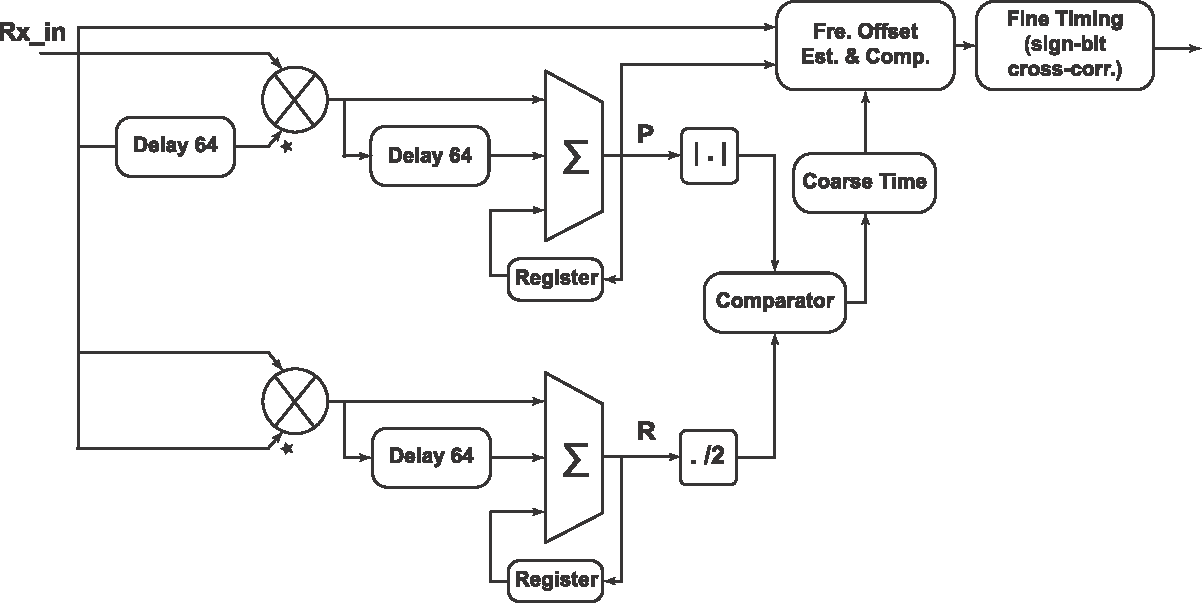
\includegraphics [width=0.8\columnwidth] {figures/Con_Sync.pdf}}
	\caption{Architecture of the conventional synchronisation FPGA implementation.}
	\label{fig:Con-Sync}
\end{figure}

We assume a 16-bit two's complement fixed point representation with 15 fractional bits (i.e. Q1.15 format in Q-notation).
The auto-correlation and squared amplitude of received samples are computed with a complex multiplier IP core that uses DSP slices.
Results are scaled to Q1.15 to reduce resource usage in subsequent pipeline stages.
Since this synchroniser is for the IEEE~802.16 preamble, the length of the delay is 64 samples.
Each element is scaled to be less than 1.0, guaranteeing that the final summation result is less than 64, needing just 7 bits for representation in two's complement.
Hence, the \emph{P} and \emph{R} values are represented in Q7.15 format.
For the $|P|$ metric, the auto-correlation uses a complex multiplier IP core to multiply the current received sample and the 64th delayed sample.
The magnitude of the \emph{P} metric is approximated to reduce hardware complexity as per \cite{Liu2009}.
For the \emph{R} metric, another complex multiplier is used to compute the squared magnitude of the received sample.
The threshold is commonly chosen to be 0.5, which can be implemented using a right shift by 1 bit \cite{Kim2008} instead of using a multiplier.
After the frame is detected, the \emph{P} metric is used to estimate and correct the fractional CFO.
A CORDIC IP core is used to determine the phase of the \emph{P} metric, and to derive the estimated fractional CFO.
The received samples are then compensated using phase accumulation and phase rotation.
These compensated samples are now used to determine fine timing synchronisation.

		\subsubsection{Implementation of Proposed Synchroniser}

\begin{figure}[h]
	\centerline{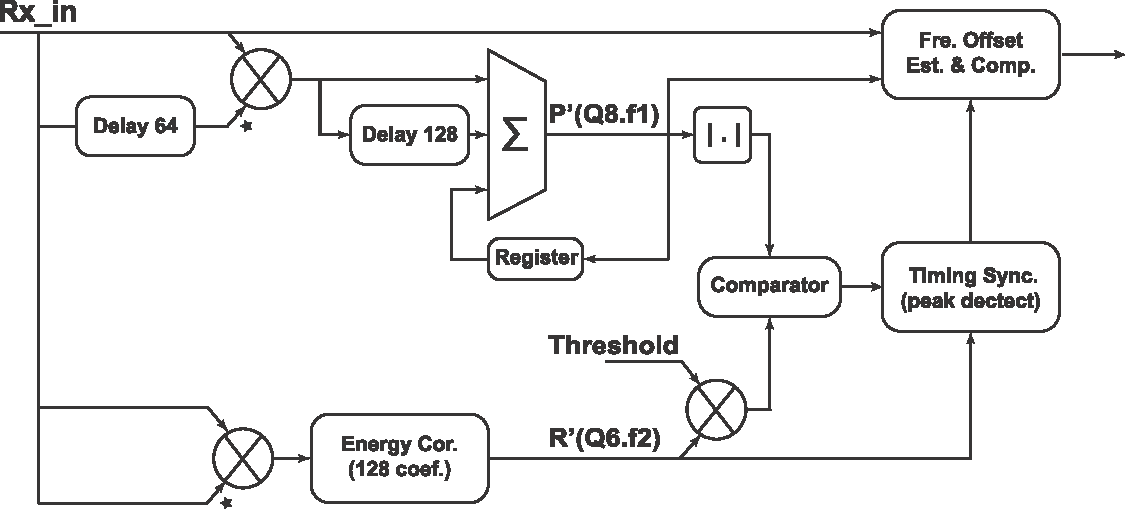
\includegraphics [width=0.8\columnwidth] {figures/Pro_Sync.pdf}}
	\caption{Architecture for the proposed synchronisation method implemented on FPGA.}
	\label{fig:Pro-Sync}
\end{figure}

The architecture for our proposed method is shown in Fig.~\ref{fig:Pro-Sync}.
The format of received samples is similar to the conventional design.
The \emph{R'} metric is determined using an energy correlator as illustrated in Fig.~\ref{fig:ML-Cor}.
The number of samples used to compute it is 128 and since the 128 samples of the short preamble are arranged in two identical spans of 64 samples each, the correlator only needs 64 taps.
The proposed method improves upon full cross-correlation not just by taking advantage of the periodic nature of the preamble, but also profiting from the real number computation of the proposed metrics, instead of requiring complex computation, and through enabling the use of a multiplierless correlator, yielding a significant computational saving.
Eqn.~(\ref{ProposedR-imp}) shows the derived equations of this optimisation:
\begin{eqnarray}
\label{ProposedR-imp}
R'(z) &=& I(z)A_{127} + I(z) z^{-1}A_{126} + ... + I(z) z^{-63}A_{64} \nonumber \\
	  &  &	+ I(z) z^{-64}A_{63} + ...+ I(z) z^{-127}A_0, \nonumber \\
	  &=& I(z)A_{63}   + I(z) z^{-1}A_{62}  +...+ I(z) z^{-63}A_0 \nonumber \\
	  &  &	+ I(z) z^{-64}A_{63} + ...+I(z) z^{-127} A_0], \nonumber \\
	  &=& (I(z)+I(z)z^{-64})A_{63} +... \nonumber \\
	  &  & 	+ (I(z)+I(z)z^{-64}) z^{-63}A_0, \nonumber \\
	  &=&I(z) (1+z^{-64})A_{63} +  z^{-1}(I(z)(1+z^{-64})A_{62}\nonumber \\
	  &	&						 + z^{-1 }( ...+z^{-1}I(z)(1+z^{-64})A_{0}))),
\end{eqnarray}
where \emph{I} is the squared amplitude of the received sample and $A_n$ denotes the normalised squared amplitude of known preambles.
Following this, a multiplierless correlator, as described in detail in \cite{Pham2012}, is used to compute the output, shown in block diagram form in Fig.~\ref{fig:ML-Cor}.

\begin{figure}[h]
	\centerline{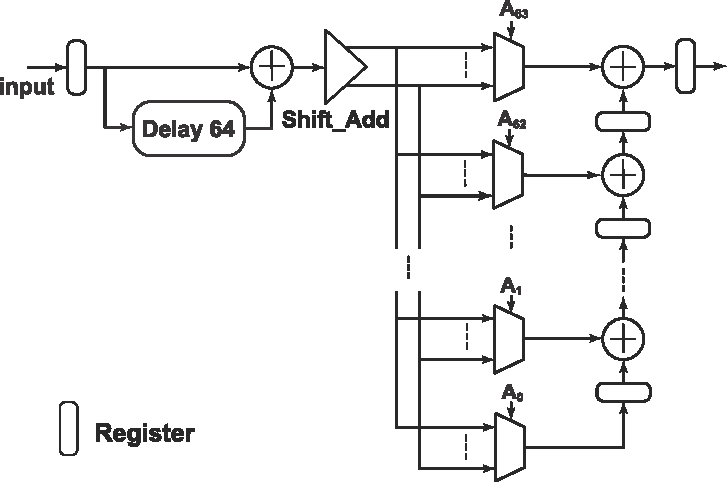
\includegraphics [width=0.6\columnwidth] {figures/ML_Cor.pdf}}
	\caption{Implementation of energy correlator on FPGA.}
	\label{fig:ML-Cor}
\end{figure}

The values of $A_n$ are quantised to 0.5 and a shift/multiplex operation replaces the multiplication.
$R'$ is always positive and smaller than twice the sum of all $A_n$ elements, i.e., 63. So the $R'$ metric requires just 6 bits to represent its integer part.

The $P'$ metric is computed in an identical way to the conventional one, but the number of samples used in the computation is 128 instead of 64 since $C=2L$.
So, the moving summation uses a delay buffer of 128 samples, and the result value now requires 8 bits to represent the integer part.

\subsubsection{Effect of Reduced Precision}

Let $f1$ and $f2$ be the number of bits representing the fractional part for computing \emph{P'}  and \emph{R'} respectively. Thus \emph{P'} has fixed point format Q8.$f1$ and \emph{R'} has fixed point format Q6.$f2$.
The effects of reducing the number of bits used to represent these fractional components of  \emph{P'}  and \emph{R'}  will now be investigated, with the aim of optimising the reduced precision against hardware savings.

Recall the results of CFO estimation in the simulation sub-section where \textit{Prop2} exhibited a significant improvement in CFO estimation accuracy compared to \textit{SoA} due to an increase in the evaluation window size obtained by setting $C=2L$. This requires more multiplications, leading to increased hardware cost to compute the \emph{P'} metric. Reducing $f1$ allows a reduction in this extra hardware cost by making each individual computation simpler. The question is to determine how much reduction in $f1$ can be sustained without losing the performance advantage enjoyed by \textit{Prop2}.

\begin{table}[hb]
	\centering
	\caption{Resources required for computing $P'$ on FPGA with different word lengths, $Q1.f1$.}
	\label{tab:P-Metric}
	\begin{tabular}{r|c|c|c|c}
        \hline \hline
    			 {$f1$}	&  {FF}	&  {LUT}  &  {BRAM} &  {DSP}\\
	\hline
		\textit{Prop-15b}	& 304 	& 427 	& 96	& 3 \\
		\textit{Prop-7 b}		& 240 	& 323	& 64 	& 3 \\
		\textit{Prop-6 b}		& 232 	& 311	& 60 	& 3 \\
		\textit{Prop-5 b}		& 224  	& 297  	& 56	& 3 \\
		\textit{Prop-4 b}		& 216  	& 269  	& 52	& 3 \\
	\hline \hline
    \end{tabular}
\end{table}

To understand precisely how $f1$ reduction can save hardware, Table~\ref{tab:P-Metric} details the hardware resource required for implementing five representative word sizes. Meanwhile, Fig. \ref{fig:Fest_AWGN_PQ} plots CFO performance curves for the corresponding sizes of $f1$. It is clear from the graph that all degraded precision computations perform well -- even the lowest Q1.4 precision computation (\textit{Prop-4b}) can outperform \textit{SoA} below about 7dB.
The optimal choice for this range of SNRs is probably $f1=7bits$ (\textit{Prop-7b}) which suffers just a slight decrease in accuracy compared to the `full length' 15 bit version (\textit{Prop-15b}). This allows a reduction of 21\%, 24\%, and 33\% in the number of flipflops (FF), Look-up-tables (LUT), and BRAM blocks, respectively. Moreover, \textit{Prop-7b} still achieves excellent performance when compared to the state of the art method, \textit{SoA}.

\begin{figure}[h]
	\centering
	\begin{tikzpicture}
	\begin{semilogyaxis}[ xlabel=SNR(dB), ylabel=MSE of Fractional CFO (\%), legend columns=2,	legend style={at={(0.5,1.02)}, anchor=south, cells={anchor=west}, draw=none}, x post scale=1.4]
		\addplot+[black, style={solid,thick},every mark/.append style={mark=*, style=solid}]  table [x index=0, y index=1] {./Dat/Fest_AWGN_Q.dat};
		\addlegendentry{\textit{SoA}};
		\addplot+[style={densely dashed,thick},every mark/.append style={mark=pentagon, style=solid}] table [x index=0, y index=2] {./Dat/Fest_AWGN_Q.dat};
		\addlegendentry{\textit{Prop-4b}};
		\addplot+[style={densely dashed,thick},every mark/.append style={mark=o, style=solid}]  table [x index=0, y index=3] {./Dat/Fest_AWGN_Q.dat};
		\addlegendentry{\textit{Prop-5b}};
		\addplot+[style={densely dashed,thick},every mark/.append style={mark=square, style=solid}]  table [x index=0, y index=4] {./Dat/Fest_AWGN_Q.dat};
		\addlegendentry{\textit{Prop-6b}};
		\addplot+[style={solid,thick},every mark/.append style={mark=diamond*, style=solid}] table [x index=0, y index=5] {./Dat/Fest_AWGN_Q.dat};
		\addlegendentry{\textit{Prop-7b}};
		\addplot+[style={densely dashed, thick},every mark/.append style={mark=triangle, style=solid}]  table [x index=0, y index=6] {./Dat/Fest_AWGN_Q.dat};
		\addlegendentry{\textit{Prop-15b}};
	\end{semilogyaxis}
	\end{tikzpicture}
	\caption{Performance of CFO estimation in an AWGN channel against SNR, with different numbers of fractional bits used in the computation of $P'$.}
\label{fig:Fest_AWGN_PQ}
\end{figure}

\begin{table}[h]
	\centering
	\caption{Resources required for computing \emph{R'} on FPGA with different word lengths, $Q1.f2$.}
	\label{tab:R-Metric}
	\begin{tabular}{r|c|c|c|c}
        \hline \hline
    			  {$f2$}	&  {FF}	& {LUT}  &  {BRAM} &  {DSP}\\
	\hline
		\textit{Prop-15b} 	& 1404 	& 1017 	& 16	& 2 \\
		\textit{Prop-7 b}		& 884 	& 633	& 8	 	& 2 \\
		\textit{Prop-6 b}		& 818 	& 589	& 7	 	& 2 \\
		\textit{Prop-5 b}		& 753  	& 537  	& 6		& 2 \\
		\textit{Prop-4 b}		& 689  	& 504  	& 5		& 2 \\
	\hline \hline
    \end{tabular}
\end{table}

\begin{figure}
	\centering
	\begin{tikzpicture}
	\begin{semilogyaxis}[ xlabel=SNR(dB), ylabel=Fail rate of frame synchronisation (\%), legend columns=2,	legend style={at={(0.5,1.02)}, anchor=south, cells={anchor=west}, draw=none}, x post scale=1.4]
		\addplot+[black, style={solid},every mark/.append style={mark=*, style=solid}]  table [x index=0, y index=1] {./Dat/FailRate_AWGN_Q.dat};
		\addlegendentry{\textit{SoA,thick}};
		\addplot+[style={densely dashed,thick},every mark/.append style={mark=pentagon, style=solid}] table [x index=0, y index=2] {./Dat/FailRate_AWGN_Q.dat};
		\addlegendentry{\textit{Prop-4b}};
		\addplot+[style={densely dashed,thick},every mark/.append style={mark=o, style=solid}]   table [x index=0, y index=3] {./Dat/FailRate_AWGN_Q.dat};
		\addlegendentry{\textit{Prop-5b}};
		\addplot+[style={solid,thick},every mark/.append style={mark=diamond*, style=solid}] table [x index=0, y index=4] {./Dat/FailRate_AWGN_Q.dat};
		\addlegendentry{\textit{Prop-6b}};
		\addplot+[style={densely dashed,thick},every mark/.append style={mark=square, style=solid}]  table [x index=0, y index=5] {./Dat/FailRate_AWGN_Q.dat};
		\addlegendentry{\textit{Prop-7b}};
		\addplot+[style={densely dashed,thick},every mark/.append style={mark=triangle, style=solid}] table [x index=0, y index=6] {./Dat/FailRate_AWGN_Q.dat};
		\addlegendentry{\textit{Prop-15b}};
	\end{semilogyaxis}
	\end{tikzpicture}
\caption{Performance of frame synchronisation in an AWGN channel against SNR, with different numbers of fractional bits used in the computation of $R'$.}
\label{fig:STO_AWGN_RQ}
\end{figure}


Similarly, the optimized tradeoff between the accuracy of STO estimation and hardware usage for computation of the \emph{R'} metric is obtained based on reducing $f2$. In this case,
Table~\ref{tab:R-Metric} reveals the corresponding reduction achieved in computation resources and Fig.~\ref{fig:STO_AWGN_RQ} plots the frame synchronisation fail rate with SNR for several values of $f2$.
The performance of the proposed method with $f2=6bit$, \textit{Prop-6b}, can be seen to be almost identical to the `full length' computation using 15 fractional bits, \textit{Prop-15b}. Overall, \textit{Prop-6b} achieves much more accurate estimation compared to the state of the art method, \textit{SoA}. Reducing $f2$ to 6 bits allows a reduction of 41\%, 42\%, and 56\% in the number of FFs, LUTs, and BRAM blocks.

		\subsubsection{Optimized Alternatives}

The preceding results are now used to define four alternative implementations of the proposed method to  compare against the state-of-the-art method, \textit{SoA} which uses full length Q1.15 arithmetic. These alternatives are namely:
\begin{itemize}
\item \textit{Prop-A1}: a non-optimized instance of the proposed method with both $f1$ and $f2$ set to 15.
\item \textit{Prop-A2}: only $P'$ is optimized with $f1$ = 7 while $f2$ remains set to 15.
\item \textit{Prop-A3}: only $R'$ is optimized with  $f2$ = 6 while $f1$ remains set to 15.
\item \textit{Prop-A4}: both $P'$ and $R'$ are optimized by setting $f1$ = 7 and $f2$ = 6.
\end{itemize}


\begin{table}[h]
	\centering
	\caption{ Total resources consumed by a full word length implementation of \textit{SoA} and four reduced complexity instances of the proposed method. Dynamic (Dpwr) and quiescent power (Qpwr) consumption are reported in mA. Maximum frequency is reported in MHz.}
	\label{tab:Int_Imp_Rpt}
	\begin{tabular}{r|c|c|c|c|c|c}
        \hline \hline
    			 {}	&  {Slices} &  {BRAM} &  {DSP}&  {Qpwr}& {Dpwr}& {Frequency}\\
	\hline
		\textit{SoA} 	& 930 	& 112 	& 13	& 37	& 41 & 121 \\
		\textit{Prop-A1}	& 1000 	& 118	& 14 	& 37 	& 43 & 133 \\
		\textit{Prop-A2}	& 923 	& 86	& 14 	& 37	& 39 & 142 \\
		\textit{Prop-A3}	& 869  	& 109  	& 14	& 37 	& 38 & 137 \\
		\textit{Prop-A4}	& 777  	& 77  	& 14	& 37 	& 35 & 142 \\
	\hline \hline
    \end{tabular}
\end{table}


Table~\ref{tab:Int_Imp_Rpt} reports the overall hardware resources required for these instances of the synchroniser, as well as detailing the power consumption of each.
It should be noted that the CFO estimation and frame synchronisation performance of these instances can be seen by choosing the corresponding word length from plots of \emph{P'} \& \emph{R'} in Figs. \ref{fig:Fest_AWGN_PQ} \& \ref{fig:STO_AWGN_RQ} respectively. In other words, all instances have been simulated and reported in the previous plots.
From the table, it is evident that reducing word length can yield a significant reduction in both hardware requirement and power consumption.
The fully optimized alternative, \textit{Prop-A4}, achieves a reduction of 16.4\%, 31.2\%, and 14.6\% in the number of occupied slices, BRAMs, and in dynamic power consumption, when compared to \textit{SoA}.
The maximum frequencies of the SoA and proposed method implementations are also reported.
The required frequency for baseband processing in IEEE~802.16 ranges from from 5.6 to 22.4~MHz, and this requirement is easily met by all tested implementations.

Table~\ref{tab:Imp_Rpt} details the comparison between \textit{SoA} and \textit{Prop-A4} in terms of their constituent building block resources (where the function names in this table correspond to the block diagrams of Figs.~\ref{fig:Con-Sync} and \ref{fig:Pro-Sync}).

\begin{table}[h]
	\centering
	\caption{ Resource comparison between two synchronisation methods.}
	\label{tab:Imp_Rpt}
	\begin{tabular}{l|r|r|r|r|r}
       \hline \hline
    		  \multicolumn{2}{r|}{Function}			& {FF} & {LUT} & {BRAM} & {DSP} \\
    	\hline
		\textit{SoA}		&  $|P|$ metric		& 303 	& 427 	& 64 	& 3 	\\
						&  $R$ metric		& 168 	& 186 	& 16 	& 2	\\
						&  CFO comp		& 1478 	& 1517 	& 0	 	& 8	\\
						& Coarse time		& 7  	& 33  	& 0	 	& 0	\\
    						& Fine time			& 942  	& 1009  	& 32 	& 0	\\
						& \textbf{Total} & \textbf{2898} & \textbf{3172} & \textbf{112} & \textbf{13}\\
	\hline
		\textit{Prop-A4}	& $|P'|$ metric		& 240 	& 323 	& 64 	& 3 \\
						& $R'$ metric		& 818 	& 600 	& 7		& 2 \\
						& CFO comp		& 1467 	& 1515 	& 0 		& 8 \\
						& Time sync			& 66	& 98	& 6 		& 1 \\
						& \textbf{Total} & \textbf{2591} & \textbf{2536} & \textbf{77} & \textbf{14}\\
    	\hline \hline
    \end{tabular}
\end{table}

The function named `CFO comp', which performs frequency offset estimation and compensation, clearly consumes the largest amount of hardware in both methods.
The \emph{R'} metric computation in \textit{Prop-A4} uses more hardware than the computation of \emph{R} in \textit{SoA}. However, fine timing estimation, `Fine time', takes a large proportion of the total hardware cost in \textit{SoA} while the alternative in the proposed method (timing synchronisation, known as `Time sync'), requires much less hardware.

%---------------------------------------------------------------------------------
\section{Summary}
%---------------------------------------------------------------------------------

Although the state of the art synchronisation methods achieve good performance when the CFO is in the range of fractional CFO estimation, they can not work with larger CFO.
Some methods employ cross-correlation for the time synchronisation; these methods are robust to large CFO and can obtain acceptable performance at low SNR.
However, the much higher computational resources needed for cross-correlation tend to make such methods unsuitable for hardware implementation.
The methods have been presented to improve upon these drawbacks of previous reported works.
The method takes the advantage of period and energy distribution characteristics of the preamble to perform time synchronisation.
The synchronisation performance results, obtained through simulation, demonstrate good performance and robustness to large CFO.
Although the method just estimates and compensates the fractional CFO, the method still performs well with larger CFO values.
An enhanced OFDM synchronisation method that provides an efficient and low cost IFO estimation will be presented in the next chapter.

\chapter{A Method for OFDM Timing Synchronisation}
\label{chap:Synchronisation}
%%!TEX root = main_thesis.tex
%---------------------------------------------------------------------------------
\chapter{A CFO Estimation Method for OFDM Synchronisation}
\label{chap:CFO}
%---------------------------------------------------------------------------------

%---------------------------------------------------------------------------------
\section{Introduction}
%---------------------------------------------------------------------------------
In the previous chapter, robust OFDM timing synchronisation was explored, leading to a proposed method that is able to perform well even in the case of large fractional CFO.
However, the CFO estimation of that method was only estimate the fractional CFO rather than large integer CFO that can occur as a result of the Doppler Effect and/or due to local oscillator instabilities.
CFO is usually normalised by subcarrier spacing and divided into an integer frequency offset (IFO) part, which is a whole multiple of subcarrier spacings, and a remainder which is referred to as fractional frequency offset (FFO).
IFO causes a circular shift of the subcarrier in the frequency domain while FFO results in ICI because of lost orthogonality between subcarriers.
\begin{figure}[b]
    \centerline{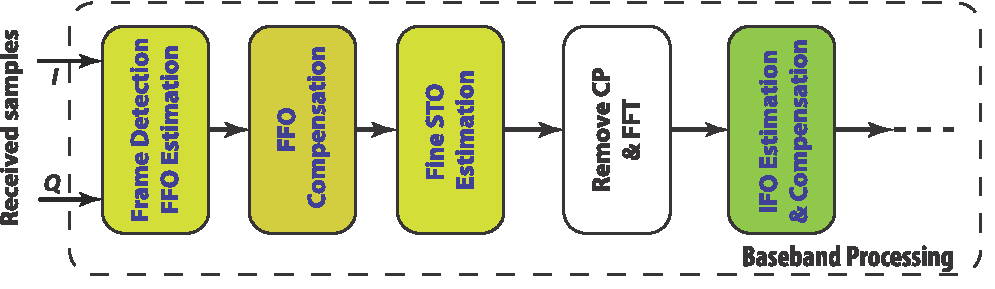
\includegraphics [width=0.9\columnwidth] {figures/Baseband.pdf} }
    \caption{Baseband processing block diagram.}
    \label{fig:baseband}
\end{figure}
Fig.~\ref{fig:baseband} illustrates the process of FFO and IFO estimation in the baseband processing of a typical OFDM system.
The IFO estimation is performed after the FFT, and relies upon cross-correlation, which consumes significant hardware resources.
A typical OFDM receiver avoids the need for IFO estimation by limiting CFO tolerance to be smaller than the range of allowable FFO estimation, resulting in a set of very strict constraints on the design of the RF front-end. However, if CFO exceeds the range of FFO estimation, IFO is present and the system cannot therefore function correctly.
This is more pronounced in applications that subject the front-end to intensive Doppler (including rapidly mobile systems), for very high carrier frequencies, or systems which aim to support multiple frequency bands for different standards.

In this chapter, a novel method is proposed for IFO estimation to overcome this challenge to efficient and low-power implementation. The basis of this method has also been discussed in:
\begin{itemize}
\item T. H. Pham, S. A. Fahmy, and I. V. McLoughlin, ``Efficient Integer Frequency Offset Estimation Architecture for Enhanced OFDM Synchronization,'' to be submitted to \textit{IEEE Transactions on Very Large Scale Integration (VLSI) Systems}.
\end{itemize}

%---------------------------------------------------------------------------------
\section{Related Work}
%---------------------------------------------------------------------------------
As mentioned in the previous chapter, the estimation range of  fractional CFO has a limitation that is shown in (\ref{fractionalCFOlimitation}); for instance its range is up to $\pm$2 sub-carrier spacings in the case of the IEEE~802.16 preamble. The value of the IFO is a multiple of the coarse CFO's range.
It is commonly estimated by performing cross-correlation \cite{Bang2001,Kim2008} in the frequency domain.

Let us assume that the signal is transmitted over a frequency selective channel that has channel impulse response (CIR) $h$ with length, \emph{L} ($L<N_{CP}$), and which is corrupted by AWGN.
The received signal, suffering frequency and timing offsets, can be expressed in the time domain as
\begin{equation}
\label{xnfull}
y[n] = \sum_{l=0}^{L-1} h[l]x[n-\tau-l] e^{i(2\pi \xi \frac{n-\tau}{N} + \phi_0)} + w[n]
\end{equation}
where $w[n]$ denotes AWGN in the time domain, $\tau$, $\phi_0$ are residual timing offset (RTO) and error phase, respectively, and $\xi$ is the normalised CFO that can be divided into an FFO part $\lambda$ and an IFO part $\epsilon$ as $\xi=\lambda+\epsilon$.

Assuming FFO and STO be compensated by earlier stages of synchronisation, as has been investigated in detail by other authors \cite{Kim2008,Pham2014}, the received preamble symbol after CP removal at FFT output is
\begin{equation}
\label{xnrec}
Y[k] =  e^{i(\phi_0-2\pi \frac{\tau k}{N})} H[k-\epsilon] X[k-\epsilon] + W[k]
\end{equation}
where $W[k]$ and $H[k]$ are the frequency domain representations of AWGN and CIR, respectively.
%\todo[inline]{**Thinh: I think it should that $W[k]$ in the above equation (ivm)}

As mentioned previously, IFO results in a cyclic shift in the frequency domain and is commonly estimated by performing cross-correlation in the frequency domain.
By contrast, RTO causes a linear phase rotation on samples in the frequency domain that may cause degradation of cross-correlation performance during IFO estimation.
Based on a differential demodulation of the FFT output, the IFO can be determined with better robustness to frequency selective channel and RTO effects using the correlation function \cite{Park2002} expressed by:

\begin{equation}
\label{integerCFO}
\hat{\epsilon} =\underset{\tilde{\epsilon}}{\operatorname{argmax}}  \left|\sum_{k=1}^{N} Y^{*}[k-1] Y[k]  X^{*}[k-\tilde{\epsilon}]  X[k-1-\tilde{\epsilon}]\right|
\end{equation}
where $(.)^{*}$ denotes complex conjugation, $\hat{\epsilon}$, $\tilde{\epsilon}$ are estimated and trial values of $\epsilon$, respectively,
$Y[k]$ and $X[k]$ denote the $k^{th}$ frequency symbol index of the received symbol and the known transmitted preamble, respectively, and the symbol size $N$ is equal to the FFT size.

The estimated IFO can achieve high precision using cross-correlation in the frequency domain, however implementing cross-correlation clearly involves a significant hardware overhead, with a multiplier needed for each element in the cross-correlation.
Sign-bit cross-correlation \cite{Schwoerer2002} is a widely adopted approach to reducing correlation complexity using only the most significant bit (MSB) of the signed two's complement numbers in the correlation computation. In this way, complexity is reduced at the cost of some performance degradation.
Despite the adoption of such methods, cross-correlation remains computationally expensive, especially when dealing with a large FFT size.
It should be noted here that several IFO estimation methods have been published which claim robustness to frequency selective channels and RTO. However, published FPGA implementations of these methods are lacking to date, possibly because the hardware costs are considerable -- even when adopting the sign-bit cross-correlation approach as mentioned.%}

There are few practical implementations for IFO estimation and correction.
A notable exception was presented in \cite{Kim2008}, in which time-domain cross correlation is performed between received samples and several pre-rotated versions of the preamble corresponding to possible IFO values. Although this method uses efficient sign-bit correlation to reduce hardware cost (at the cost of decreased estimation accuracy and increased sensitive to frequency
selective channels), it is not efficient when the possible IFO range is large since it effectively performs an exhaustive search of possibilities.

State of the art OFDM synchronisation methods typically have a small tolerance of CFO that requires the hardware be strictly constrained to ensure operation within a small CFO range which does not include any IFO.
This strict timing requirement leads to an increase in total system cost. Particularly, in the case of MSCR, the need for high precision timing, coupled with a requirement for a wide ranging and agile operating frequency span, would make the RF front-end design extremely difficult, if not impossible.

%---------------------------------------------------------------------------------
\section{Enhanced OFDM Synchronization Through Novel IFO Estimation Architecture}
%---------------------------------------------------------------------------------
In this section, we propose a novel method in which hardware resources and power consumption are reduced by determining IFO estimates for only a subset of possible IFO values. This in turn enables an efficient resource sharing folded architecture to be adopted. Adjusting the precision of individual correlation computations within this novel architecture leads to a fine degree of control on the trade-off between performance and power consumption.
The implementation uses the long preamble of IEEE~802.16-2009~\cite{IEEE80216} for estimating IFO values.
This preamble has a symbol size of 256 with 100 pilots, as illustrated in Fig.~\ref{fig:long_pre}.
These 100 pilots are distributed, 50 pilots per side, at even sub-carrier spacings from 2 to 100 and from 156 to 254. The remaining sub-carriers are null.
\begin{figure}[b]
    \centerline{\includegraphics [width=1\columnwidth] {figures/long_pre.pdf} }
    \caption{Pilots in the long preamble of IEEE~802.16-2009.}
    \label{fig:long_pre}
\end{figure}
In OFDM-based systems such as 802.11, 802.16, and 802.22, the short preamble is used to estimate and compensate for FFO.
Typically, fractional CFO estimation has a limited range of up to ${\pm}2$ sub-carrier spacings depending on the format of the short preamble.
This results in the possible IFO values being a multiple of 4. The limitation of fractional CFO and the possible IFO values are discussed in detail in the previous chapter.
It should be noted that, although the proposed method is applied to 802.16 for evaluating the accuracy of IFO estimation, it can be applied in other OFDM-based systems having similar preamble structures, such as 802.11 and 802.22.

\subsection{Proposed Algorithm}
%\begin{itemize}
Firstly, a subset of possible IFO values is determined.
We assume that the RF front end can provide CFO stability in a range from -14 to +18 subcarrier spacings, which is relaxed compared to the strict RF front end constraints in 802.16 that would typically otherwise lead to increased RF hardware costs.
Generally, the larger the range of IFO estimation that is performed, the larger the CFO that the baseband system can tolerate.
A wider CFO tolerance in turn leads to a relaxation in RF front-end specification, hence reducing system cost.
In this system, there are 8 possible values for IFO estimation in the assumed CFO range.
The subset of possible IFO values is denoted $S_{IFO} = \{-12, -8, -4, 0, 4, 8, 12, 16\}$.  Moreover, samples are pre-offset by 12 subcarrier spacings prior to calculation to ensure that all possible values of IFO are positive, $S'_{IFO} = \{0:4:28\}$.
This means that received symbols will only ever need to be shifted right to compensate IFO, thus reducing buffer memory requirements.

Secondly, a resource sharing folded architecture is designed to significantly reduce the hardware cost.
Conventionally, to obtain high accuracy, IFO estimation is computed across all pilots in the preamble.
This results in considerable hardware overhead, especially with a large number of pilots, as is the case for IEEE~802.16-2009.
Evidently, as the number of pilots increases, the correlation result shows greater robustness to noise.
However, we will demonstrate in Section \ref{sec:Sim} that the beneficial effect of calculating across additional pilots leads to decreasing gains in performance.
In fact the performance improvement reaches a plateau.
We therefore propose making use of only a subset of pilots, while maintaining estimation accuracy as much as possible.
Then, by spreading the chosen subset of pilots carefully in the time domain, it becomes possible to design a resource-sharing architecture for computing the cross-correlation, hence reducing area and power consumption.
When the proposed method is applied to IEEE~802.16-2009 offset estimation, the pilots used for the IFO computation are selected at subcarrier indices that are multiples of 4, leading to a natural four-fold resource sharing architecture.
Hence, the IFO estimation can be expressed as:
\begin{equation}
\label{integerCFOprop}
\hat{\epsilon} =\underset{\tilde{\epsilon} \in S'_{IFO}}{\operatorname{argmax}}  \left|\sum_{k=1}^{N/4} P(4k)  A(4k-\tilde{\epsilon})\right|
\end{equation}
where $P(4k) = Y^{*}(4k-2) Y(4k)$ denotes the correlation of two consecutive received pilots, and $A(4k) = X(4k-2) X^{*}(4k)$ is the correlation of two consecutive transmitted pilots that can be pre-computed.

Thirdly, although sign-bit cross-correlation is often used in conventional implementations~\cite{Kim2008,Schwoerer2002}, as it can significantly reduce computational complexity, it also leads to reduced precision and hence reduced estimation performance, especially in the case of frequency selective channels.
For this reason, we instead apply multiplierless correlation to enhance the accuracy of estimation (i.e. using several bits for computation, rather than the existing extremes of either a single sign bit or a full word computation).
In \cite{Pham2012}, we authors demonstrated a trade-off between cost and accuracy for multiplierless OFDM synchronisation.
We further investigate this effect in the current chapter in terms of the trade-off between cost and accuracy when reducing the wordlength used to represent $P(4k)$.

\subsection{Proposed Architecture}
\label{subsec:Imple}
The proposed method divides IFO estimation into multiple repeated computations with resource sharing based upon the four-sample timing between selected spread pilots.
The estimation of IFO in (\ref{integerCFO}) can now be rewritten as follows
\begin{eqnarray}
\label{proposedimplementIFO}
\hat{\epsilon}  &=&\underset{\tilde{\epsilon} \in S'_{IFO}}{\operatorname{argmax}}  \left|V_{\tilde{\epsilon}}  \right|,	 \nonumber \\
V_{\tilde{\epsilon}} &=& \sum_{k=0}^{25} P(4k) A_{\tilde{\epsilon}}(4k) + P(L+4k)  A_{\tilde{\epsilon}}(L+4k),
\end{eqnarray}
where $A_{\tilde{\epsilon}}$ denotes the correlation of two consecutive pre-rotated known pilots corresponding to one IFO value, and $V_{\tilde{\epsilon}}$ is the cross-correlation between received pilots and pre-rotated known pilots.
Since the pilots of the long preamble are distributed on two sides of the OFDM symbol in the frequency domain, at even sub-carrier spacings from 2 to 100 and 156 to 254, \emph{L} denotes the index of the first pilots in second half.
In the case of IEEE~802.16, \emph{L} equals 156.
Each value, $V_{\tilde{\epsilon}}$, can be computed simultaneously and separately using a multi-add accumulation scheme.
The challenge in implementation is find a way to efficiently share resources when computing $V_{\tilde{\epsilon}}$.
The pilots that are used to compute the correlation arrive every four cycles so there are four spare cycles between two consecutive computed pilots, allowing one multiply accumulate block to sequentially compute 4 separate correlations.

There are 8 sets of $A_{\tilde{\epsilon}}$ corresponding to 8 possible IFOs.
These sets of $A_{\tilde{\epsilon}}$ can be pre-computed and stored separately.
Thanks to the spreading of the computed pilots, the $A_{\tilde{\epsilon}}$ sets have many identical pilots -- this naturally allows sharing between pre-rotated pilot sets -- so that only 64 memory locations are required instead of 400. Thus, an 84\% reduction in the memory used to store $A_{\tilde{\epsilon}}$ sets is achieved.
Fig.~\ref{fig:Pilots} illustrates the $A_{\tilde{\epsilon}}$ sets and circuitry for combining all $A_{\tilde{\epsilon}}$ sets.
\begin{figure}
	\centerline{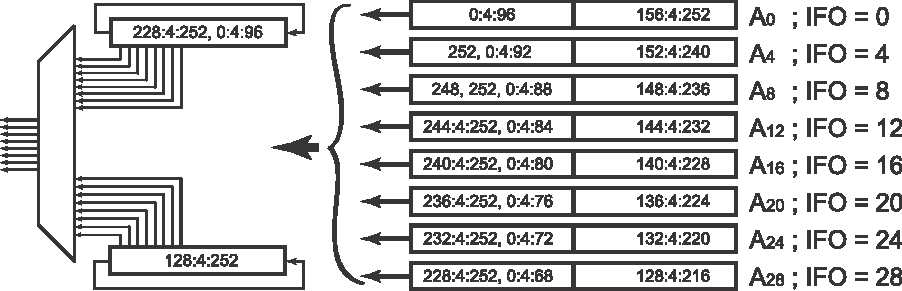
\includegraphics [width=1\columnwidth] {figures/Pilots.pdf} }
	\caption{Circuit for the known-pilots shift register.}
	\label{fig:Pilots}
\end{figure}
%Due to the 4 sample offset between consecutive pilots used for computation, four-fold resource sharing can naturally be performed at the same clock rate for computation of $V_{i}$.

Multiply accumulate blocks are shared for computing four sequential $V_{\tilde{\epsilon}}$ values over four successive clock periods. Fig.~\ref{fig:subsampling} demonstrates how this is done. $P_k$ is received in every clock cycle. $P_{4k}$ is the subsampling of $P_k$, taking a subset of the most significant bits from $P_k$ every four cycles. The cross-correlation is performed with the values of $P_{4k}$. Two multipliers, \emph{M1} and \emph{M2} are used to compute the values of 8 cross-correlations $V_{\tilde{\epsilon}}$ in parallel. Each multiplier performs multiplications sequentially between $P_{4k}$ and the corresponding transmitted pilots in 4 sets of $A_{\tilde{\epsilon}}$. The products are accumulated to the values of $V_{\tilde{\epsilon}}$. When all pilots are computed, the maximum operation, $argmax|V|$, is performed on 8 $V_{\tilde{\epsilon}}$ values to estimate the IFO.

\begin{figure}
	\centerline{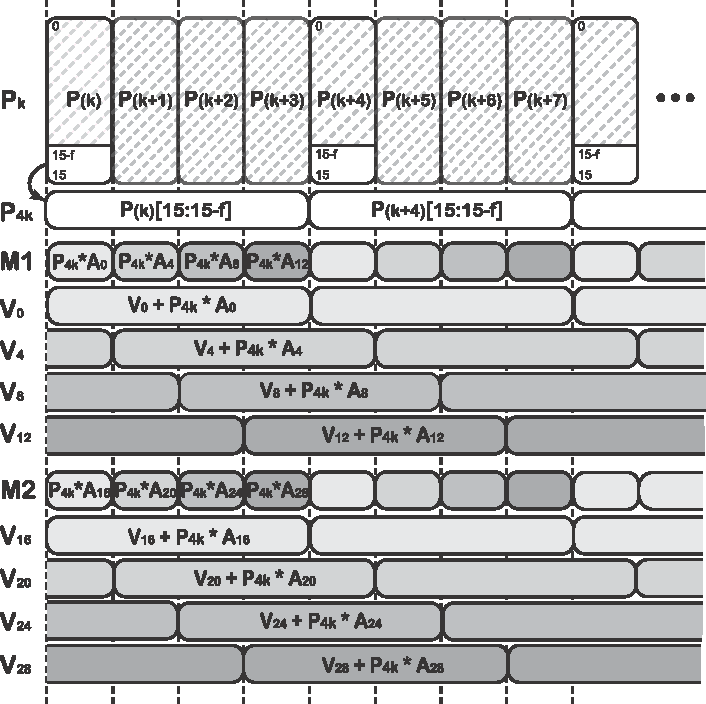
\includegraphics [width=1\columnwidth] {figures/Subsampling.pdf} }
	\caption{Resource sharing approach for computing $V_{\tilde{\epsilon}}$.}
	\label{fig:subsampling}
\end{figure}


\begin{figure}
	\centerline{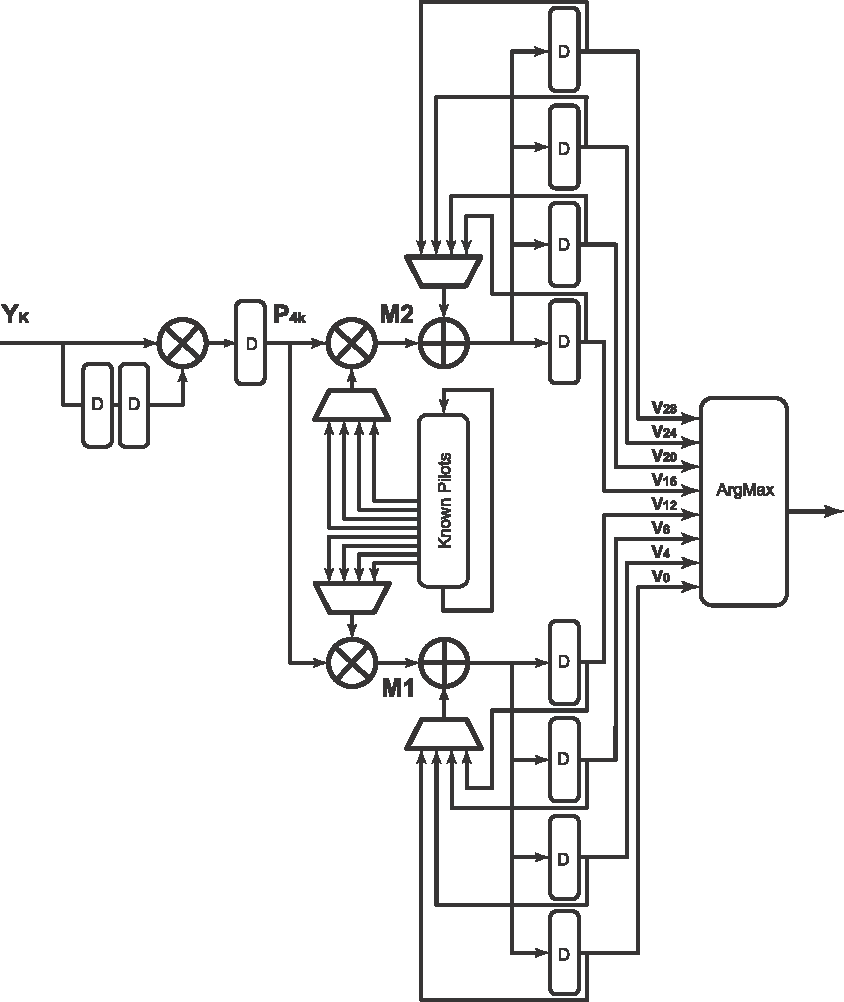
\includegraphics [width=0.95\columnwidth] {figures/ProposedStruc2.pdf} }
	\caption{Architecture of proposed IFO estimator.}
	\label{fig:ProposedStruc}
\end{figure}

To design an optimised architecture for IFO estimation, the multiply-add formula of $V_{\tilde{\epsilon}}$ is mathematically manipulated into what is effectively a multiply-accumulate form.
When one received sample is taken, $V_{\tilde{\epsilon}}$ can be expressed in the form of accumulations as in
\begin{eqnarray}
\label{complexVi}
V_{\tilde{\epsilon}}(n)	&=&   A_{\tilde{\epsilon}}(n) P(n)  + V_{\tilde{\epsilon}}(n-1), \nonumber \\
	 %&=&  (\Re{\{R\}}+i \Im{\{R\}}) (\Re{\{P_i\}} - i \Im{\{P_i\} }) \nonumber\\
	%&  &   + (\Re{\{Acc\}}+i \Im{\{Acc\}}),
						&=& (\Re{\{C_A\}} - i \Im{\{C_A\}})  (\Re{\{P(n)\}} + i \Im{\{P(n)\}}) \nonumber \\
	 					&  &+ (\Re{\{V_{\tilde{\epsilon}}(n-1)\}}+i \Im{\{V_{\tilde{\epsilon}}(n-1)\}})
\end{eqnarray}
where $\Re{\{.\}}$ and $\Im{\{.\}}$ denote the real and imaginary parts, respectively, and \emph{P(n)}, $A_{\tilde{\epsilon}}(n)$ denote the current values of the correlation of two consecutive received pilots and corresponding transmitted pilots, respectively.
$V_{\tilde{\epsilon}}(n-1)$ is the accumulated value of $V_{\tilde{\epsilon}}$.
To employ multiplierless correlation, $A_{\tilde{\epsilon}}$ are normalized to values $C_A$ whose real and imaginary parts have values in \{-1, 0, 1\}, and the wordlength of \emph{P(n)} and $V_{\tilde{\epsilon}}$ in fixed point format can be adjusted to increase estimation accuracy at the cost of increased hardware resource consumption.
The real and imaginary parts of $V_{\tilde{\epsilon}}$ can then be computed as
\begin{eqnarray}
\label{realimaginaryVi}
\Re{\{V_{\tilde{\epsilon}}(n)\}} &=& \Re{\{C_A\}} \Re{\{ P(n)\}}+\Im{\{C_A\}} \Im{\{ P(n)\}} \nonumber \\
								& &+ \Re{\{V_{\tilde{\epsilon}}(n-1)\}} , 					\nonumber \\
\Im{\{V_{\tilde{\epsilon}}(n)\}} &=& \Re{\{C_A\}} \Im{\{ P(n)\}}-\Im{\{C_A\}} \Re{\{ P(n)\}}	\nonumber \\
								& &+ \Im{\{V_{\tilde{\epsilon}}(n-1)\}}
\end{eqnarray}

The proposed resource sharing architecture for the IFO estimator is shown in Fig.~\ref{fig:ProposedStruc}. The \emph{ArgMax} module finds the maximum of the 8 $V_{\tilde{\epsilon}}$ values in order to identify the corresponding IFO estimate.
The novelty of this IFO estimator is in terms of algorithmic improvements and architecture optimisation. This is achieved by firstly reformulating the equation into an expression that is computable with efficient shared resource circuitry.
Thanks to the significant hardware reduction achieved, this IFO estimator can be feasibly implemented on a low-power, limited hardware resource FPGA, while simultaneously ensuring that performance is maintained by a trade off between number of pilots against word length.

We are able to demonstrate that the algorithm and structure optimisations mentioned above retain competitive estimation accuracy compared to conventional approaches, while also offering significant reductions in hardware resource usage.
This makes it possible to implement a high-performance OFDM receiver on a low-power FPGA, especially where the available number of DSP blocks is limited.

\subsection{Simulation}
\label{sec:Sim}
Many variants of the proposed method were simulated in MATLAB using different channel models and the parameter set of the IEEE~802.16-2009 downlink preamble. Performance of the implementation was compared to the theoretical performance of some state of the art methods.
This was assessed primarily in terms of the probability of failed estimation (POFE) with respect to channel SNR.
POFE, which is widely used to evaluate the performance of IFO estimation~\cite{Park2002,Shim2006,Morelli2008}, measures the number of fail estimations divided by the total number of IFO estimations.
Overall, 100,000 IFO estimations were simulated in AWGN and Stanford University Interim (SUI)~\cite{V.ErcegJuly2003} frequency selective channels.
IFO estimation is performed with non-ideal FFO compensation, and FFO is determined and compensated using the method of Kim and Park~\cite{Kim2008}.
The simulation also verifies the performance of the proposed method under the effect of RTO caused by imperfect STO estimation (assuming that STO estimation is still within the CP and does not cause ISI).
In addition, a randomly generated amount of STO is added in the range from 0 to $N_{CP}-L-1$, where \emph{L} is the length of CIR.

We first investigate the performance degradation compared to theoretical performance as a result of reducing the number of pilots as proposed. Next, we will investigate the effect of wordlength optimisation.
In both cases, comparisons are made with established methods in the literature that can be simulated but are otherwise infeasible for hardware implementation, namely the conventional method in \cite{Park2002} (\emph{PCH}) that is applied to one training block with 100 pilots.
In addition,  two state of the art methods are also simulated for comparison.
Firstly, metric \emph{SY} from \cite{Shim2006} as defined by,

\begin{eqnarray}
\label{equ:SY}
\hat{\epsilon} &=&\underset{\tilde{\epsilon} \in S_{IFO}}{\operatorname{argmax}} \left| \mu_{_{SY}}(\tilde{\epsilon})  \right|,	 \nonumber \\
\mu_{_{SY}}(\tilde{\epsilon}) &=& \Re{\left\{\sum_{k=1}^{\frac{N}{2}} Y^{*}_{(2k-2)} Y_{(2k)}  X^{*}_{(2k-\tilde{\epsilon})} X_{(2k-2-\tilde{\epsilon})}\right\}}
\end{eqnarray}
Secondly, metric \emph{MM} from \cite{Morelli2008},

%\todo[inline]{**Thinh -  the equation above doesn't include  $\hat{\epsilon}$ and is very similar to the next equation -- is there some problem? (ivm)}
\begin{eqnarray}
\label{equ:MM}
\hat{\epsilon} &=& \underset{\tilde{\epsilon} \in S_{IFO}}{\operatorname{argmax}} \left| \mu_{_{MM}}(\tilde{\epsilon}) \right|,	 \nonumber \\
\mu_{_{MM}}(\tilde{\epsilon}) &=& \Re{\left\{e^{i\frac{\pi}{4}} \sum_{k=1}^{\frac{N}{2}} Y^{*}_{(2k-2)} Y_{(2k)}  X^{*}_{(2k-\tilde{\epsilon})}  X_{(2k-2-\tilde{\epsilon})}\right\}}
\end{eqnarray}
where $\Re{\{.\}}$ denotes the real part.

We are unaware of any published circuits for these methods, because of their complex computation. The very large hardware requirement for these respective metrics does not lend either method to feasible implementation on a low cost, low power FPGA (unlike the proposed method).

\subsubsection{Performance Comparison}

The performance of the proposed method, denoted \emph{Prop}, is evaluated in comparison to the theoretical performance of state of the art methods by Park et. al.~\cite{Park2002}, Shim and You~\cite{Shim2006} and Morelli and Moretti~\cite{Morelli2008}, denoted \emph{PCH}, \emph{SY} and \emph{MM}, respectively in the previous subsection.
The theoretical performance is computed with full precision using full multiplication.
However, it must be noted that implementing this directly in hardware would be prohibitive due to the large number of multiplication operations needed.
In fact, hardware implementation would conventionally use sign-bit correlation instead of full precision correlation, as mentioned previously. Thus the full multiplication results shown here are undoubtedly better than those achievable in practice, and thus can be considered as upper performance bounds.
For more realistic data, we also provide results from sign-bit correlation versions of the above, denoted
\emph{PCH\_sb}, \emph{SY\_sb}, and \emph{MM\_sb} respectively.

The proposed method, evaluated against these, uses 50 spread pilots with indices that are multiples of 4.
For the sake of comparison, an additional implementation of \emph{PCH} is reported which, like the proposed method, uses only 50 pilots, but which are placed continuously rather than being spread. This is denoted \emph{PCH\_50}.
Figs.~\ref{fig:IFO_AWGN} and \ref{fig:IFO_AWGN_RTO} plot performance results for all methods in an AWGN channel, with and without RTO respectively, and reveal that the proposed method generally performs well, especially at higher SNRs. Considering more realistic channel models, Figs.~\ref{fig:IFO_SUI1} and \ref{fig:IFO_SUI2} plot the performance of all methods in SUI1, and SUI2 channels respectively, and similarly show that the proposed method performs well, especially at higher SNRs.


\begin{figure}
	\centering
	\begin{tikzpicture}
	\begin{semilogyaxis}[ xlabel=SNR(dB), ylabel=Probability of Fail Estimation (\%), legend columns=4,	legend style={at={(0.5,1.02)}, anchor=south, cells={anchor=west}, draw=none},
						 xmax=12, ymin=0.001, ymax=100, x post scale=1.4]
		\addplot+[black, style={dashed},every mark/.append style={mark=square, style=solid}] 		 table [x index=0, y index=1] {./Dat/AWGN_cmp_meth.dat};
		\addlegendentry{MM};
		\addplot+[black, style={dotted},	every mark/.append style={mark=square, style=solid}]		 table [x index=0, y index=2] {./Dat/AWGN_cmp_meth.dat};
		\addlegendentry{MM\_sb};
		\addplot+[black, style={dashed},	every mark/.append style={mark=diamond, style=solid}]	 table [x index=0, y index=3] {./Dat/AWGN_cmp_meth.dat};
		\addlegendentry{SY};
		\addplot+[black, style={dotted},	every mark/.append style={mark=diamond, style=solid}]	 table [x index=0, y index=4] {./Dat/AWGN_cmp_meth.dat};
		\addlegendentry{SY\_sb};
		\addplot+[black, style={dashed},	every mark/.append style={mark=triangle, style=solid}] 	 table [x index=0, y index=5] {./Dat/AWGN_cmp_meth.dat};
		\addlegendentry{PCH};
		\addplot+[black, style={dotted},	every mark/.append style={mark=triangle, style=solid}]	 table [x index=0, y index=6] {./Dat/AWGN_cmp_meth.dat};
		\addlegendentry{PCH\_sb};
		\addplot+[black, style={solid},	every mark/.append style={mark=o, style=solid}]			 table [x index=0, y index=7] {./Dat/AWGN_cmp_meth.dat};
		\addlegendentry{PCH\_50};
		\addplot+[black, style={solid},	every mark/.append style={mark=*, style=solid}]			 table [x index=0, y index=8] {./Dat/AWGN_cmp_meth.dat};
		\addlegendentry{Prop};
	\end{semilogyaxis}
	\end{tikzpicture}
\caption{Fail rate of IFO estimation methods in AWGN channel without RTO.}
\label{fig:IFO_AWGN}
\end{figure}

% add new figure for IFO estimation with RTO
\begin{figure}
	\centering
	\begin{tikzpicture}
	\begin{semilogyaxis}[ xlabel=SNR(dB), ylabel=Probability of Fail Estimation (\%), legend columns=4,	legend style={at={(0.5,1.02)}, anchor=south, cells={anchor=west}, draw=none},
						 xmax=12, ymin=0.001, ymax=100, x post scale=1.4]
		\addplot+[black, style={dashed},every mark/.append style={mark=square, style=solid}] 		 table [x index=0, y index=1] {./Dat/AWGN_cmp_meth_toff.dat};
		\addlegendentry{MM};
		\addplot+[black, style={dotted},	every mark/.append style={mark=square, style=solid}]		 table [x index=0, y index=2] {./Dat/AWGN_cmp_meth_toff.dat};
		\addlegendentry{MM\_sb};
		\addplot+[black, style={dashed},	every mark/.append style={mark=diamond, style=solid}]	 table [x index=0, y index=3] {./Dat/AWGN_cmp_meth_toff.dat};
		\addlegendentry{SY};
		\addplot+[black, style={dotted},	every mark/.append style={mark=diamond, style=solid}]	 table [x index=0, y index=4] {./Dat/AWGN_cmp_meth_toff.dat};
		\addlegendentry{SY\_sb};
		\addplot+[black, style={dashed},	every mark/.append style={mark=triangle, style=solid}] 	 table [x index=0, y index=5] {./Dat/AWGN_cmp_meth_toff.dat};
		\addlegendentry{PCH};
		\addplot+[black, style={dotted},	every mark/.append style={mark=triangle, style=solid}]	 table [x index=0, y index=6] {./Dat/AWGN_cmp_meth_toff.dat};
		\addlegendentry{PCH\_sb};
		\addplot+[black, style={solid},	every mark/.append style={mark=o, style=solid}]			 table [x index=0, y index=7] {./Dat/AWGN_cmp_meth_toff.dat};
		\addlegendentry{PCH\_50};
		\addplot+[black, style={solid},	every mark/.append style={mark=*, style=solid}]			 table [x index=0, y index=8] {./Dat/AWGN_cmp_meth_toff.dat};
		\addlegendentry{Prop};
	\end{semilogyaxis}
	\end{tikzpicture}
\caption{Fail rate of IFO estimation methods in AWGN channel with RTO.}
\label{fig:IFO_AWGN_RTO}
\end{figure}
%==

\begin{figure}
	\centering
	\begin{tikzpicture}
	\begin{semilogyaxis}[ xlabel=SNR(dB), ylabel=Probability of Fail Estimation (\%), legend columns=4,	legend style={at={(0.5,1.02)}, anchor=south, cells={anchor=west}, draw=none},
						 xmax=12, ymin=0.001, ymax=100, x post scale=1.4]
		\addplot+[black, style={dashed},every mark/.append style={mark=square, style=solid}] 		 table [x index=0, y index=1] {./Dat/SUI1_cmp_meth.dat};
		\addlegendentry{MM};
		\addplot+[black, style={dotted},	every mark/.append style={mark=square, style=solid}]		 table [x index=0, y index=2] {./Dat/SUI1_cmp_meth.dat};
		\addlegendentry{MM\_sb};
		\addplot+[black, style={dashed},	every mark/.append style={mark=diamond, style=solid}]	 table [x index=0, y index=3] {./Dat/SUI1_cmp_meth.dat};
		\addlegendentry{SY};
		\addplot+[black, style={dotted},	every mark/.append style={mark=diamond, style=solid}]	 table [x index=0, y index=4] {./Dat/SUI1_cmp_meth.dat};
		\addlegendentry{SY\_sb};
		\addplot+[black, style={dashed},	every mark/.append style={mark=triangle, style=solid}] 	 table [x index=0, y index=5] {./Dat/SUI1_cmp_meth.dat};
		\addlegendentry{PCH};
		\addplot+[black, style={dotted},	every mark/.append style={mark=triangle, style=solid}]	 table [x index=0, y index=6] {./Dat/SUI1_cmp_meth.dat};
		\addlegendentry{PCH\_sb};
		\addplot+[black, style={solid},	every mark/.append style={mark=o, style=solid}]			 table [x index=0, y index=7] {./Dat/SUI1_cmp_meth.dat};
		\addlegendentry{PCH\_50};
		\addplot+[black, style={solid},	every mark/.append style={mark=*, style=solid}]			 table [x index=0, y index=8] {./Dat/SUI1_cmp_meth.dat};
		\addlegendentry{Prop};
	\end{semilogyaxis}
	\end{tikzpicture}
\caption{Fail rate of IFO estimation methods in SUI1 channel.}
\label{fig:IFO_SUI1}
\end{figure}

\begin{figure}
	\centering
	\begin{tikzpicture}
	\begin{semilogyaxis}[ xlabel=SNR(dB), ylabel=Probability of Fail Estimation (\%), legend columns=4,	legend style={at={(0.5,1.02)}, anchor=south, cells={anchor=west}, draw=none},
						 xmax=12, ymin=0.001, ymax=100, x post scale=1.4]
		\addplot+[black, style={dashed},every mark/.append style={mark=square, style=solid}] 		 table [x index=0, y index=1] {./Dat/SUI2_cmp_meth.dat};
		\addlegendentry{MM};
		\addplot+[black, style={dotted},	every mark/.append style={mark=square, style=solid}]		 table [x index=0, y index=2] {./Dat/SUI2_cmp_meth.dat};
		\addlegendentry{MM\_sb};
		\addplot+[black, style={dashed},	every mark/.append style={mark=diamond, style=solid}]	 table [x index=0, y index=3] {./Dat/SUI2_cmp_meth.dat};
		\addlegendentry{SY};
		\addplot+[black, style={dotted},	every mark/.append style={mark=diamond, style=solid}]	 table [x index=0, y index=4] {./Dat/SUI2_cmp_meth.dat};
		\addlegendentry{SY\_sb};
		\addplot+[black, style={dashed},	every mark/.append style={mark=triangle, style=solid}] 	 table [x index=0, y index=5] {./Dat/SUI2_cmp_meth.dat};
		\addlegendentry{PCH};
		\addplot+[black, style={dotted},	every mark/.append style={mark=triangle, style=solid}]	 table [x index=0, y index=6] {./Dat/SUI2_cmp_meth.dat};
		\addlegendentry{PCH\_sb};
		\addplot+[black, style={solid},	every mark/.append style={mark=o, style=solid}]			 table [x index=0, y index=7] {./Dat/SUI2_cmp_meth.dat};
		\addlegendentry{PCH\_50};
		\addplot+[black, style={solid},	every mark/.append style={mark=*, style=solid}]			 table [x index=0, y index=8] {./Dat/SUI2_cmp_meth.dat};
		\addlegendentry{Prop};
	\end{semilogyaxis}
	\end{tikzpicture}
\caption{Fail rate of IFO estimation methods in SUI2 channel.}
\label{fig:IFO_SUI2}
\end{figure}

Under these experimental conditions, \emph{PCH} and \emph{SY} achieve equivalent performance in AWGN without RTO and in SUI1 channels.
However, \emph{SY} degrades more drastically than \emph{PCH} in the SUI2 channel at SNRs above 1\,dB.
\emph{SY} also deteriorates in the case of AWGN with RTO. This method appears to be very sensitive to large RTO, while \emph{MM} and \emph{PCH} exhibit better robustness to RTO.
The accuracy of \emph{MM} is slightly lower than that of \emph{PCH} at SNRs below 0\,dB, while performance is very similar at larger SNRs.
Also note the performance of the conventional approach implementations, \emph{PCH\_sb}, \emph{SY\_sb}, \emph{MM\_sb} which degrade significantly with SNR, especially in the SUI1, SUI2 channels.

Apart from at very low SNRs, the proposed method, \emph{Prop}, achieves almost identical performance to the simulated upper bound \emph{PCH}, even in the presence of RTO.
It should be noted that \emph{Prop} achieves this while allowing the use of resource sharing through sparse pilot computation. This will be used below to achieve a significant hardware saving.
According to simulation results, \emph{Prop}, with its spread pilots, is also more accurate than \emph{PCH\_50} that uses the same number of pilots, but places them continuously.

\subsubsection{Wordlength Optimisation}
Since sign-bit correlation degrades IFO estimation performance, specially in frequency selective channels, the proposed method instead employs multiplierless correlation to improve accuracy and robustness.
The complexity of this approach is dependent on the wordlength chosen for the correlation computation.
We now investigate how wordlength affects the performance of the proposed implementation, again compared to the theoretical bound, \emph{PCH}, as well as to the performance of a conventional sign-bit implementation, \emph{PCH\_sb}.
We denote wordlength using the notation $Q1.f$, meaning a single integer bit and $f$ fractional bits.
Evaluations are performed for $f$ of 1, 2, 7, and 15 bits. These results will be plotted in the following figures with the labels \emph{Prop\_1b}, \emph{Prop\_2b}, \emph{Prop\_7b}, and \emph{Prop\_15b}, respectively.
Figs.~\ref{fig:IFO_Qb_AWGN} and \ref{fig:IFO_Qb_AWGN_RTO} plot the performance in AWGN (with and without RTO), with all tested wordlengths in the proposed method performing comparably to \emph{PCH} (and being much better than \emph{PCH\_sb} at SNRs exceeding about 2\,dB).
Figs.~\ref{fig:IFO_Qb_SUI1} and \ref{fig:IFO_Qb_SUI2} plot the results when using the more realistic SUI1 and SUI2 channel models.

\begin{figure}
	\centering
	\begin{tikzpicture}
	\begin{semilogyaxis}[ xlabel=SNR(dB), ylabel=Probability of Fail Estimation (\%), legend columns=3,	legend style={at={(0.5,1.02)}, anchor=south, cells={anchor=west}, draw=none},
						 xmax=12, ymin=0.001, ymax=100, x post scale=1.4]
		\addplot+[black, style={dashed},	every mark/.append style={mark=triangle, style=solid}] 	 table [x index=0, y index=1] {./Dat/AWGN_Qb.dat};
		\addlegendentry{PCH};
		\addplot+[black, style={dotted},	every mark/.append style={mark=triangle, style=solid}]	 table [x index=0, y index=2] {./Dat/AWGN_Qb.dat};
		\addlegendentry{PCH\_sb};
		\addplot+[black, style={dashed}, every mark/.append style={mark=square, style=solid}] 	 table [x index=0, y index=3] {./Dat/AWGN_Qb.dat};
		\addlegendentry{Prop\_15b};
		\addplot+[black, style={dashed},	every mark/.append style={mark=diamond, style=solid}]	 table [x index=0, y index=4] {./Dat/AWGN_Qb.dat};
		\addlegendentry{Prop\_7b};
		\addplot+[black, style={solid},	every mark/.append style={mark=*, style=solid}]			 table [x index=0, y index=5] {./Dat/AWGN_Qb.dat};
		\addlegendentry{Prop\_2b};
		\addplot+[black, style={dashed},	every mark/.append style={mark=o, style=solid}]			 table [x index=0, y index=6] {./Dat/AWGN_Qb.dat};
		\addlegendentry{Prop\_1b};
	\end{semilogyaxis}
	\end{tikzpicture}
\caption{Fail rate for different wordlengths in AWGN channel without RTO.}
\label{fig:IFO_Qb_AWGN}
\end{figure}

\begin{figure}
\centering
	\begin{tikzpicture}
	\begin{semilogyaxis}[ xlabel=SNR(dB), ylabel=Probability of Fail Estimation (\%), legend columns=3,	legend style={at={(0.5,1.02)}, anchor=south, cells={anchor=west}, draw=none},
						 xmax=12, ymin=0.001, ymax=100, x post scale=1.4]
		\addplot+[black, style={dashed},	every mark/.append style={mark=triangle, style=solid}] 	 table [x index=0, y index=1] {./Dat/AWGN_Qb_toff.dat};
		\addlegendentry{PCH};
		\addplot+[black, style={dotted},	every mark/.append style={mark=triangle, style=solid}]	 table [x index=0, y index=2] {./Dat/AWGN_Qb_toff.dat};
		\addlegendentry{PCH\_sb};
		\addplot+[black, style={dashed}, every mark/.append style={mark=square, style=solid}] 	 table [x index=0, y index=3] {./Dat/AWGN_Qb_toff.dat};
		\addlegendentry{Prop\_15b};
		\addplot+[black, style={dashed},	every mark/.append style={mark=diamond, style=solid}]	 table [x index=0, y index=4] {./Dat/AWGN_Qb_toff.dat};
		\addlegendentry{Prop\_7b};
		\addplot+[black, style={solid},	every mark/.append style={mark=*, style=solid}]			 table [x index=0, y index=5] {./Dat/AWGN_Qb_toff.dat};
		\addlegendentry{Prop\_2b};
		\addplot+[black, style={dashed},	every mark/.append style={mark=o, style=solid}]			 table [x index=0, y index=6] {./Dat/AWGN_Qb_toff.dat};
		\addlegendentry{Prop\_1b};
	\end{semilogyaxis}
	\end{tikzpicture}
\caption{Fail rate for different wordlengths in AWGN channel with RTO.}
\label{fig:IFO_Qb_AWGN_RTO}
\end{figure}

\begin{figure}
\centering
	\begin{tikzpicture}
	\begin{semilogyaxis}[ xlabel=SNR(dB), ylabel=Probability of Fail Estimation (\%), legend columns=3,	legend style={at={(0.5,1.02)}, anchor=south, cells={anchor=west}, draw=none},
						 xmax=12, ymin=0.001, ymax=100, x post scale=1.4]
		\addplot+[black, style={dashed},	every mark/.append style={mark=triangle, style=solid}] 	 table [x index=0, y index=1] {./Dat/SUI1_Qb.dat};
		\addlegendentry{PCH};
		\addplot+[black, style={dotted},	every mark/.append style={mark=triangle, style=solid}]	 table [x index=0, y index=2] {./Dat/SUI1_Qb.dat};
		\addlegendentry{PCH\_sb};
		\addplot+[black, style={dashed}, every mark/.append style={mark=square, style=solid}] 	 table [x index=0, y index=3] {./Dat/SUI1_Qb.dat};
		\addlegendentry{Prop\_15b};
		\addplot+[black, style={dashed},	every mark/.append style={mark=diamond, style=solid}]	 table [x index=0, y index=4] {./Dat/SUI1_Qb.dat};
		\addlegendentry{Prop\_7b};
		\addplot+[black, style={solid},	every mark/.append style={mark=*, style=solid}]			 table [x index=0, y index=5] {./Dat/SUI1_Qb.dat};
		\addlegendentry{Prop\_2b};
		\addplot+[black, style={dashed},	every mark/.append style={mark=o, style=solid}]			 table [x index=0, y index=6] {./Dat/SUI1_Qb.dat};
		\addlegendentry{Prop\_1b};
	\end{semilogyaxis}
	\end{tikzpicture}
\caption{Fail rate for different wordlengths in SUI1 channel.}
\label{fig:IFO_Qb_SUI1}
\end{figure}

\begin{figure}
\centering
	\begin{tikzpicture}
	\begin{semilogyaxis}[ xlabel=SNR(dB), ylabel=Probability of Fail Estimation (\%), legend columns=3,	legend style={at={(0.5,1.02)}, anchor=south, cells={anchor=west}, draw=none},
						 xmax=12, ymin=0.001, ymax=100, x post scale=1.4]
		\addplot+[black, style={dashed},	every mark/.append style={mark=triangle, style=solid}] 	 table [x index=0, y index=1] {./Dat/SUI2_Qb.dat};
		\addlegendentry{PCH};
		\addplot+[black, style={dotted},	every mark/.append style={mark=triangle, style=solid}]	 table [x index=0, y index=2] {./Dat/SUI2_Qb.dat};
		\addlegendentry{PCH\_sb};
		\addplot+[black, style={dashed}, every mark/.append style={mark=square, style=solid}] 	 table [x index=0, y index=3] {./Dat/SUI2_Qb.dat};
		\addlegendentry{Prop\_15b};
		\addplot+[black, style={dashed},	every mark/.append style={mark=diamond, style=solid}]	 table [x index=0, y index=4] {./Dat/SUI2_Qb.dat};
		\addlegendentry{Prop\_7b};
		\addplot+[black, style={solid},	every mark/.append style={mark=*, style=solid}]			 table [x index=0, y index=5] {./Dat/SUI2_Qb.dat};
		\addlegendentry{Prop\_2b};
		\addplot+[black, style={dashed},	every mark/.append style={mark=o, style=solid}]			 table [x index=0, y index=6] {./Dat/SUI2_Qb.dat};
		\addlegendentry{Prop\_1b};
	\end{semilogyaxis}
	\end{tikzpicture}
\caption{Fail rate for different wordlengths in SUI2 channel.}
\label{fig:IFO_Qb_SUI2}
\end{figure}

It can be seen from the plots that each of the tested wordlengths achieves much better performance and exhibits greater robustness to frequency selective channels than the sign-bit realisation of the conventional approach, \emph{PCH\_sb}.
Additionally, these realisations of the proposed method do not suffer as much degradation in the presence of RTO.
Moreover, it is possible to improve low SNR performance by adopting a longer wordlength with the proposed method, at a cost of increased hardware complexity. Increasing wordlength does improve results slightly, with the step from 1 to 2 bits being the most significant gain. By contrast, increasing from 2 to 7 or from 7 to 15 bits has little impact.
In general, \emph{Prop\_2b} achieves an estimation accuracy close to that of the theoretical performance bound, \emph{PCH}, at intermediate and higher SNRs, even though it involves computation with fewer bits, and can hence be implemented more efficiently.

%---------------------------------------------------------------------------------------------------------------------------------------------------------------------
\subsection{FPGA Implementation}
\label{sec:Imple}
The analysis in Section~\ref{sec:Sim} suggests that the proposed method offers comparable estimation performance to existing methods in the literature.
As a result of the simplifications inherent in the proposed approach, this should be achievable at a reduced hardware cost.
This section now quantifies this hardware cost, for an FPGA-based implementation.
It is important to note that these hardware savings are accessible for a number of target implementation devices, although we are interested primarily in FPGA implementation as part of our work on leveraging FPGA reconfigurability in cognitive radios.

\subsubsection{Conventional Approach}
To obtain the theoretical performance previously discussed in Section \ref{sec:Sim} and denoted as \emph{PCH}, the computation of the estimation metric in \cite{Park2002}, using 100 pilots, would require about 200 complex multipliers, resulting in the use of over 600 DSP blocks. This may exceed the available resources on small devices, or leave insufficient resources for other tasks on larger devices.
As the number of multiplications required for a full implementation of the approach is prohibitive, the conventional approach for implementation, as we have discussed, uses sign-bit correlation~\cite{Kim2008}.
This conventional implementation uses all 100 pilots in the long preamble to perform sign-bit correlation, and multiply\_adds are eliminated at taps where the pilots of the long preamble are not used.
This implementation mirrors the \emph{PCH\_sb} in Section \ref{sec:Sim}, and allows us to quantify the benefits of our proposed approach against a known reference benchmark.

\subsubsection{Proposed Approach}

The proposed architecture for the IFO estimator, implemented with several different wordlengths of $P(n)$ and $V_{\tilde{\epsilon}}$ in (\ref{complexVi}), are compared to allow us to explore the hardware costs associated with the respective implementations.
Four fixed point formats for $P(n)$, are investigated: Q1.1, Q1.2, Q1.7, and Q1.15.
$V_{\tilde{\epsilon}}$  is represented accordingly in Q7.1, Q7.2, Q7.7, and Q7.15 formats to avoid overflow.

In order to obtain a comprehensive optimised implementation, these circuits are each implemented using two different structures.
The first uses only logic elements (LE) for computation, while the second uses Xilinx DSP48A1 \cite{ug389} primitives.
Considering (\ref{realimaginaryVi}), $\Re{\{V_{\tilde{\epsilon}}(n)\}}, \Im{\{V_{\tilde{\epsilon}}(n)\}}$ can be computed effectively using two DSP blocks as 3-input adders, instead of 4 blocks as would be usual.
Fig.~\ref{fig:DSP48Acc} illustrates how this is done for $\Re{\{V_{\tilde{\epsilon}}(n)\}}$, and similarly for $\Im{\{V_{\tilde{\epsilon}}(n)\}}$.
\begin{figure}
	\centerline{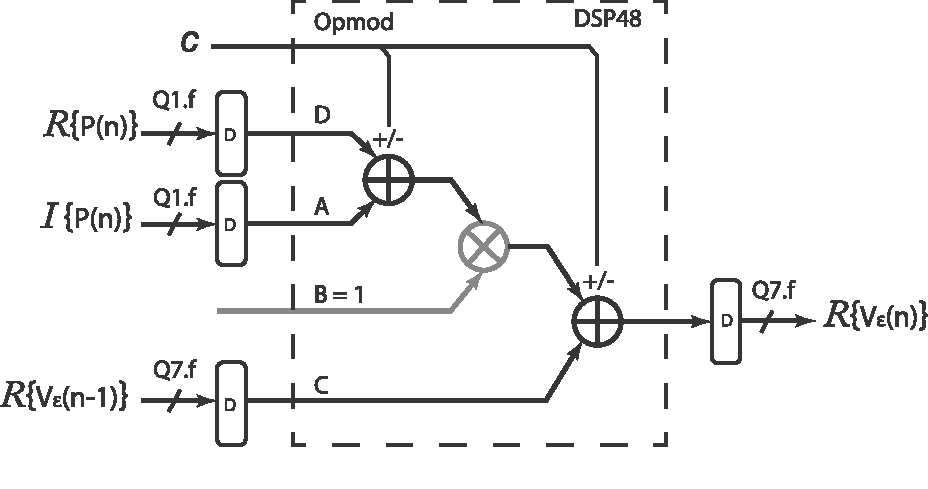
\includegraphics [width=1\columnwidth] {figures/DSP48Acc.pdf} }
	\caption{DSP block based 3-input adder for correlation.}
	\label{fig:DSP48Acc}
\end{figure}
Note that the solution presented in Fig.~\ref{fig:DSP48Acc} is optimised for QPSK modulated pilots (since their amplitudes are identical) as specified in IEEE~802.16, as well as in most OFDM-based standards.
The normalisation performed in (\ref{realimaginaryVi}) allows the correlation to be reduced to two DSP blocks operating as 3-input adders (instead of 4 DSP blocks with multipliers as would be usual).
These methods correspond to \emph{Prop\_1b}, \emph{Prop\_2b}, \emph{Prop\_7b}, and \emph{Prop\_15b} that were investigated for estimation accuracy in Section~\ref{sec:Sim}.

\subsection{Implementation Results}
The circuits were synthesised and fully implemented using Xilinx ISE 13.2, targeting the low-power Xilinx Spartan-6 XC6SLX75T FPGA.
The results are reported in terms of the number of flip-flops (FF), look-up tables (LUT), and DSP48 blocks, along with dynamic power consumption, as summarised in Table~\ref{tab:Imp_Rpt}.
\begin{table}[h]
	\centering
	\caption{Resource utilisation and dynamic power consumption of IFO estimators.}
	\label{tab:Imp_Rpt}
	\renewcommand{\arraystretch}{1.2}

	\begin{tabular}{r|r|r|r|r|r}

       \hline \hline
    		  \makebox[1.1cm][c]{IFO est. Cir.} 	& \#FF & \#LUT  & \#DSP & Fre (MHz) & D. Power \\
    	\hline
		\textbf{conv\_100p}		& 3270 (3\%)	& 1837 (3\%)	& 3 &  142 	&  42	mW \\
		Prop\_1b\_LE			& 328 (1\%)		& 370 (1\%)		& 3 &  136 	&  9		mW\\
		\textbf{Prop\_2b\_LE}	& 350 (1\%)		& 390 (1\%)		& 3 &  136 	&  10 	mW\\
		Prop\_7b\_LE			& 460 (1\%)		& 471 (1\%)		& 3 &  136 	&  12 	mW\\
		Prop\_15b\_LE		      & 735 (1\%)		& 696 (1\%)		& 3 &  134 	&  17 	mW\\

		Prop\_1b\_DSP			& 328 (1\%)		& 306 (1\%)		& 7 &  78   	&  11 	mW\\
		Prop\_2b\_DSP			& 350 (1\%)		& 319 (1\%)		& 7 &  78   	&  12	mW\\
		Prop\_7b\_DSP			& 460 (1\%)		& 379 (1\%)		& 7 &  77   	&  14	mW\\
		Prop\_15b\_DSP			& 735 (1\%)		& 591 (1\%)		& 7 &  77 	&  18 	mW\\
    	\hline \hline
    \end{tabular}
\end{table}

%\todo[inline]{**Thinh: the table above (table 5.1) has some corrupted row titles - you should either increase the row widths or remove all the width specifiers. (ivm)}

\emph{conv\_100p} refers to the conventional approach, implemented using sign-bit correlation over 100 pilots.
\emph{Prop\_fb\_LE}, \emph{Prop\_fb\_DSP}, in which $f$ = 1, 2, 7 and 15 (corresponding to received sample format Q1.$f$), denote the circuits of corresponding wordlengths, implemented using logic elements and DSP48 blocks, respectively.
Referring to the table, the proposed implementation shows that significant improvement in resource usage and dynamic power consumption is possible with the proposed method.

The hardware resources used by \emph{Prop\_fb\_LE} and \emph{Prop\_fb\_DSP} increase gradually, in terms of FFs and LUTs, as the wordlength increases.
The number of FFs used in \emph{Prop\_fb\_DSP} and \emph{Prop\_fb\_LE} is equal, while \emph{Prop\_fb\_DSP} uses fewer LUTs since the DSP blocks are used for the 3-input additions.

The \emph{Prop\_fb\_LE} implementations use 3 DSP blocks to compute $P(n)$, while \emph{Prop\_fb\_DSP} require an additional 4 DSP blocks to perform the correlation.
\emph{Prop\_fb\_LE}, \emph{Prop\_fb\_DSP} both consume far fewer LUT and FF resources than the conventional \emph{conv\_100p} implementation.

For \emph{Prop\_2b\_LE}, the number of FFs and LUTs is reduced by 90\% and 79\% respectively compared to the conventional \emph{conv\_100p} approach.

The maximum frequencies of circuits, reported after place and route, comfortably exceed the timing requirements for IEEE~802.16 synchronisation whose sampling frequency is below 25~MHz.
A post-place-and-route simulation was used to estimate the power consumption of the system at a clock rate of 50{\thinspace}MHz, using the Xilinx XPower tool -- also shown in table \ref{tab:Imp_Rpt}.

\emph{Prop\_fb\_LE} implementations consume less power than the equivalent \emph{Prop\_fb\_DSP} implementations.
All implementations of the proposed method consume significantly less power than the conventional implementation.
\emph{Prop\_2b\_LE} consumes just 22\% of the power consumed by \emph{conv\_100p}.

In subsection \ref{sec:Sim}, we established that \emph{Prop\_2b\_LE} easily outperforms the conventional approach in terms of estimation accuracy.
In this subsection, we have shown that it does so with a significant hardware resource saving, and with significantly reduced power consumption.
In fact, the estimation performance of \emph{Prop\_2b\_LE}, in AWGN and SUI channels (except at very low SNR), is close to the theoretical bound of \emph{PCH}, which would demand a significant proportion of the FPGAs resources if it were implemented conventionally.
Meanwhile, \emph{Prop\_2b\_LE} is extremely efficient, consuming less than 1\% of the resources available on a low-power Spartan-6 XC6SLX75 FPGA.
Beyond IEEE 802.16-2009, the folded resource sharing architecture, which leverages sub-sample spaced OFDM pilots, can be adopted for use in other OFDM standards (including IEEE 802.11 and IEEE 802.22).

%---------------------------------------------------------------------------------
\section{Summary}
%---------------------------------------------------------------------------------

This chapter investigated IFO estimation in OFDM-based systems such as IEEE 802.16. A technique is proposed for efficient implementation of IFO estimation, which aims in particular for a low power and low resource utilisation.
Since IFO estimation contributes significantly to the complexity of a robust synchroniser design, this work is important for multistandard radios, or applications where significant frequency variation is expected. Robust IFO estimation allows for relaxed analogue RF constraints, leading to reduced cost. A modified timing metric is derived which allows for resource sharing to reduce both resource requirements as well as power consumption. The proposed implementation makes use of a four-fold resource sharing architecture to significantly reduce hardware cost, while multiplierless correlation with optimised wordlength is used to improve estimation accuracy in comparison to a conventional implementation approach using signbit correlation.
The method is shown to perform as well as current state-of-the-art methods that employ multiplier-based correlation, and yet with significantly improved power and resource requirements. Dynamic power consumption is reduced by 78\% over even a sign-bit version of the conventional approach, yet it offers better estimation performance in both AWGN and frequency selective channels.
Beyond IEEE 802.16-2009, the folded resource sharing method, which leverages sub-sample spaced OFDM pilots, can be adopted for use in other OFDM standards (including IEEE 802.11 and IEEE 802.22). Multiplierless correlation with word length optimisation is already used within communication systems, however the trade off between the number of pilots and computational accuracy for timing synchronisation is relatively unexplored in the research literature to date.

\chapter{A CFO Estimation Method for OFDM Synchronisation}
\label{chap:CFO}
%%---------------------------------------------------------------------------------
\chapter{A Spectrum Efficient Shaping Method for OFDM Radios}
\label{chap:SpectralLeakage}
%---------------------------------------------------------------------------------

%---------------------------------------------------------------------------------
\section{Introduction}
\label{Sec:Intro}
%---------------------------------------------------------------------------------

This chapter is concerned with the OFDM spectral leakage challenge for OFDM-based CRs.
OFDM signals typically cause large amounts spectral leakage, whereas CRs demand a shaped spectrum confined within the allocated channel in order to reuse free spectral bands without causing ICI to other users occupying adjacent bands.
Some recent OFDM-based standards are defined with the requirements on spectral leakage that are extremely stringent in an effort  to avoid ICI.
Spectral leakage filtering may cause some effects on transmitted signals that lead to a reduction in the effective timing guard.
Therefore, the implementations of spectral leakage filtering need to be able to take into account the parameters of the underlying OFDM signal and its channel characteristics to avoid causing the negative effects on the transmitted signal such as distorsion and ISI.

In this chapter, a novel method that embeds baseband filtering within a cognitive radio (CR) architecture, is proposed.
The method is able to meet the specification for the most stringent 802.11p SEM, meet the specification of the 802.11af strict SEM requirement, and furthermore is able to allow ten additional 802.11af sub-carriers to occupy a single basic channel without violating SEM specifications.
In addition, the method can adaptively change filter performance according to the transmission power to reduce the computation cost while guaranteeing that the emission spectrum remains smaller than the allowed spectral leakage.
The method, performed at baseband, relaxes the otherwise strict RF front-end requirements.
This allows the RF subsystem to be implemented based upon much less stringent 802.11a designs, which can significantly reduce total cost.

The work presented in this chapter has also been discussed in:
\begin{itemize}
\item  T. H. Pham, I. V. McLoughlin, and S. A. Fahmy, ``Shaping Spectral Leakage for IEEE 802.11p Vehicular Communications,'' to appear in \textit{Proceedings of IEEE Vehicular Technology Conference (VTC Spring), Seoul, Korea, May 2014}~\cite{PhamMay2014}.
\item T. H. Pham, S. A. Fahmy, and I. V. McLoughlin, ``Spectrally Efficient Emission Mask Shaping for OFDM Cognitive Radios,''  to be submitted to \textit{IEEE Transactions on Communications (TCOM)}.
\end{itemize}

%---------------------------------------------------------------------------------
\section{Signal Model for Spectral Leakage Filtering}
\label{sec:SigMod}
%---------------------------------------------------------------------------------
Conventionally, there are two methods that can be employed to compress the spectral leakage for OFDM-based system, namely pulse shaping and image spectrum compression. Pulse shaping, recommended in 802.11a, is effective at reducing side lobes. Spectral leakage filtering is designed with respect to the signal model and channel model to avoid the negative effect of filter. In this section, we present the OFDM signal model, 802.11p and 802.11af channel models for compressing the spectral leakage.

\subsection{Signal Model}
We define an OFDM symbol to have inverse fast Fourier transform (IFFT) length and cyclic prefix (CP) length $N$ and $N_{CP}$, respectively, so that the length of the symbol including its CP is $N_{T} = N + N_{CP}$.
A sample $x(m)$ of the OFDM symbol $(0\leq m \leq N_{T}-1)$ can be expressed in the time domain as
\begin{equation}
\label{xm}
x(m) = \frac{1}{N}\sum_{k=0}^{N-1} X(k) e^{i2\pi\frac{k}{N}(m-N_{CP})},
\end{equation}
where $X(k)$ denotes the frequency domain representation of the data sub-carriers.
Since OFDM symbol samples are generally transmitted sequentially, this is equivalent to multiplying symbols with a rectangular window function, $p$.
Then the transmitted OFDM samples can be expressed as
\begin{equation}
\label{xn2}
x(n) = \frac{1}{N}\sum_{l=-\infty}^{\infty} \sum_{k=0}^{N-1} X(k) p(n-l N_{T}) e^{i2\pi\frac{k}{N}(n-N_{CP}-l N_{T}).}
\end{equation}
In a conventional OFDM system, the window function, $p(m)$, is rectangular and simply described as
\begin{equation}
\label{pm}
 p(m) =\begin{cases}1, & m = 0,1, ..., N_{T} \\  0, & otherwise \end{cases}
\end{equation}

CIR, of length $h$, is derived from the delay spread of the channel.
If the CP is shorter than the channel delay, ISI will be present in received symbols.
Channels experienced by the two standards discussed in this chapter will obviously differ, but both tend to experience high levels of delay spread: 802.11p because it is primarily a vehicular communications standard, and 802.11af because it operates in lower attenuation UHF and VHF bands.


The PHYs specified in 802.11p and 802.11af are largely inherited from the well-established 802.11a and 802.11ac OFDM PHYs, respectively.
The major parameters of both new PHYs are presented in Table~\ref{tab:Para}.
However, since the new standards operate in different channel regions and environments, they are subject to different, and much more stringent SEM requirements than their parent standards.
\begin{table}[h]
	\centering
	\caption{ Major parameters of 802.11p and 802.11af OFDM PHYs}
	\label{tab:Para}
	\renewcommand{\arraystretch}{1.2}
	\begin{tabular}{l|c|c|c|c}
		Parameters                      	 		& 802.11p & \multicolumn{3}{c}{802.11af} \\ \hline
		Bandwidth, MHz                  		& 10     & 6    & 7   & 8    \\ \hline
		Used subcarriers, $N_{C}$ 		& 52      & \multicolumn{3}{c}{114}      \\ \hline
		Total subcarriers, $N_{T}$  		& 64      & 144      & 168     & 144     \\ \hline
		FFT points, $N_{FFT}$      		& 64      & \multicolumn{3}{c}{128}      \\ \hline
		Subcarrier spacing $\Delta f$, MHz        	& ${10}/{64}$   & ${6}/{144}$    & ${7}/{168}$   & ${8}/{144}$   \\ \hline
		Sampling frequency, MHz			& 10 & 5.33 & 5.33 & 7.11  \\ \hline
		Fourier transform size         		& 6.4 us  & 24 us    & 24 us   & 18 us   \\ \hline
		CP length                        			& 1.6 us  & 6 us     & 6 us    & 4.5 us
	\end{tabular}
\end{table}

\subsection{802.11p Signal and Channel Models}

802.11p is defined for vehicular channels that tends to experience a larger delay spread than WLAN.
While the 802.11p symbol has 16 samples for CP (i.e. the same as in 802.11a), the guard intervals are lengthened to avoid ISI by reducing the bandwidth from 20\,MHz to 10\,MHz (i.e., a 10\,MHz sampling frequency). However this raises some challenges in the frequency domain.
First, reducing bandwidth requires a higher quality factor front-end filter circuit for the higher frequency carrier compared to 802.11a.
Second, 802.11p shares a 6 sub-carrier spacing frequency guard per side with 802.11a. Given the reduced sampling frequency, this leads to the absolute frequency guard being correspondingly narrower.

Generally, vehicular communication channels with large delay spread will require an increased timing guard, hence narrowing the frequency guard, which leads to more strict filtering constraints.
Empirical channel models in \cite{Acosta-Marum2007,Sen2008} reveal how maximum delay spread varies depending on different propagation models and traffic environments.
For example, the RTV model for suburban street, urban canyon, and expressway have maximum excess delays of 700, 501, and 401\,ns, respectively~\cite{Acosta-Marum2007}.
For the V2V model, measurements in \cite{Sen2008} reveal that the 90\% largest delay spread (found in urban areas) is near 600\,ns, which is equivalent to 6 samples.
Given the fact that the CP is 16 samples, this leaves 10 samples (1~us) remaining. Any spectral leakage filtering necessary to meet the stringent SEM specification must not encroach further than this into the guard time.

\subsection{802.11af Signal and Channel Models}

On the other hand, 802.11af is defined to reuse white space in the UHF band, with three basic channel units (BCUs) of 6\,MHz, 7\,MHz, and 8\,MHz.
Within this chapter, we will confine our consideration to the narrowest (and hence possibly most problematic) 6\,MHz BCU for investigating the performance of the proposed filtering method for 802.11af.

In the 802.11af channel, the measured delay spread is less than 1\,us \cite{Lan2013}, which  is equivalent to the duration of 6 samples in the CP.
Therefore, the 802.11af guard interval of 6\,us is sufficient to avoid ISI, with the remaining 5\,us (i.e., 26 samples) being available for filtering spectral leakage, if necessary.
In the US, FCC rules mandate a very strict SEM to avoid ICI on the adjacent channels of primary users in the UHF band.
For 6\,MHz channels, the signal transmitted by TVBDs shall maintain at least 55\,dB attenuation at the edge of the channel, which is significantly higher than the requirement of the parent 802.11ac standard. In the UK, the Ofcom requirement for 8\,MHz channels is similarly strict.

%---------------------------------------------------------------------------------
\section{Related Work}
%---------------------------------------------------------------------------------

This section investigates state of the art methods from the 802.11a and 802.11ac domain, and considers their application for the newer standards.
Specifically, each method is evaluated, and shown as unsuitable in meeting the strict SEM criteria for 802.11p (and hence very unlikely to satisfy the even more stringent 802.11af SEM).

\subsection{Pulse Shaping}
\label{subsec:Pulse}
%This section investigates the possibility of using pulse shaping technique to achieve the requirement of 802.11p's SEMs.
%Pulse shaping is a technique in which a smoother transition pulse is used instead of a rectangular pulse as in conventional OFDM, resulting in compressed side lobes.
Pulse shaping (using a smooth rather than rectangular pulse), recommended in 802.11a, is effective at reducing side lobes, although it induces distortion in the subcarriers.
One way to avoid the distortion is to add extending parts, i.e. CP and cyclic suffix (CS), concatenated to the conventional OFDM symbol before the beginning and after the end respectively. The extended symbol is then multiplied with a smoothing function.
While the CP in conventional OFDM is used as a guard interval, here it is also occupied, along with the CS, for pulse shaping.

Pulse shaping extends the  $N_{T}$ length of the OFDM signal by a roll-off factor, $\beta$.
One effect of extending the symbol is to reduce spectral efficiency, and thus the CP and CS of consecutive symbols can be overlapped, as shown in Fig.~\ref{fig:PS}. This, in turn, causes ISI in the overlapped region.

In practical terms, pulse shaping using the overlapping method is effectively shortening the OFDM guard interval.
A larger $\beta$ means reduced spectral leakage, at the cost of reducing the effective guard interval since a number of guard interval samples are taken for pulse shaping.
If $\beta N_{T}$ is increased to equal the CP length, the effective guard interval is reduced to zero (i.e. there is no guard interval to prevent channel-induced ISI).
In this chapter, three state-of-the-art smoothing functions for pulse shaping are investigated. We present each in discrete form, before investigating their performance with different roll-off factors.
The first smoothing function, denoted $p_1$, is present in the IEEE~802.11a standard:

%{\small
\begin{eqnarray}
\label{p1m}
&p_1 &=\begin{cases}	sin^2( \frac{\pi}{2}(0.5+\frac{m}{2\beta N_{T}}) ), 			& 0 \leq m < \beta N_{T} \\
					 	1, 															& \beta N_{T} \leq m < N_{T}  \\
					 	sin^2( \frac{\pi}{2}(0.5-\frac{m-N_{T}}{2\beta N_{T}}) ), 	& N_{T} \leq m < (1+\beta)N_{T} \end{cases}
\end{eqnarray}
%}

The second, proposed by Bala et al.~\cite{Bala2013}, is based on a raised cosine function, denoted here as $p_2$:

%{\small
\begin{eqnarray}
\label{p2m}
&p_2 &=\begin{cases}	\frac{1}{2}+\frac{1}{2}cos(\pi(1+\frac{m}{\beta N_{T}})), 			&0\leq m<\beta N_{T} \\
					 	1, 																	&\beta N_{T}\leq m < N_{T}  \\
					 	\frac{1}{2}+\frac{1}{2}cos(\pi(1+\frac{m-N_{T}}{\beta N_{T}})),		& N_{T}\leq m<(1+\beta)N_{T} \end{cases}
\end{eqnarray}
%}

The third, denoted $p_3$, is based on the characteristics of functions with vestigial symmetry as derived by Castanheira and Gameiro~\cite{Castanheira2013}:

%{\small
\begin{eqnarray}
\label{p3m}
&p_3 &=\begin{cases}	\frac{1}{2}+\frac{9}{16}cos( \pi(1 - \frac{m}{\beta N_{T}}) ) & \\
						- \frac{1}{16}cos(3\pi(1 - \frac{m}{\beta N_{T}}) ), 					& 0 \leq m < \beta N_{T} \\
					 	1, 																	& \beta N_{T} \leq m < N_{T}  \\
					 	\frac{1}{2}+\frac{9}{16}cos( \pi \frac{m-N_{T}}{\beta N_{T}}) &\\
						-\frac{1}{16}cos(3\pi \frac{m-N_{T}}{\beta N_{T}}),					&  N_{T} \leq m < (1+\beta)N_{T} \end{cases}
\end{eqnarray}
%}

The compression of OFDM spectral side lobes as a consequence of pulse shaping is investigated by first assuming that the effect of the image spectrum caused by interpolation or digital-to-analogue conversion (DAC) is negligible.
This assumption is noted because the band gap between the wanted spectrum and its image is relatively narrow.
Thus the overlapping image spectrum can influence the effectiveness of the shaped spectral leakage.
The issue will be discussed later in the chapter, where image cancellation is presented separately for 802.11p and 802.11af.

The three smoothing functions are simulated for otherwise identical channels and signals, and compared in Fig.~\ref{fig:Spec_PS}. The figure reveals the spectral envelope attenuation achieved using the three smoothing functions. %, with respect to the transmitted OFDM symbol.

\begin{figure}[t]
    \centerline{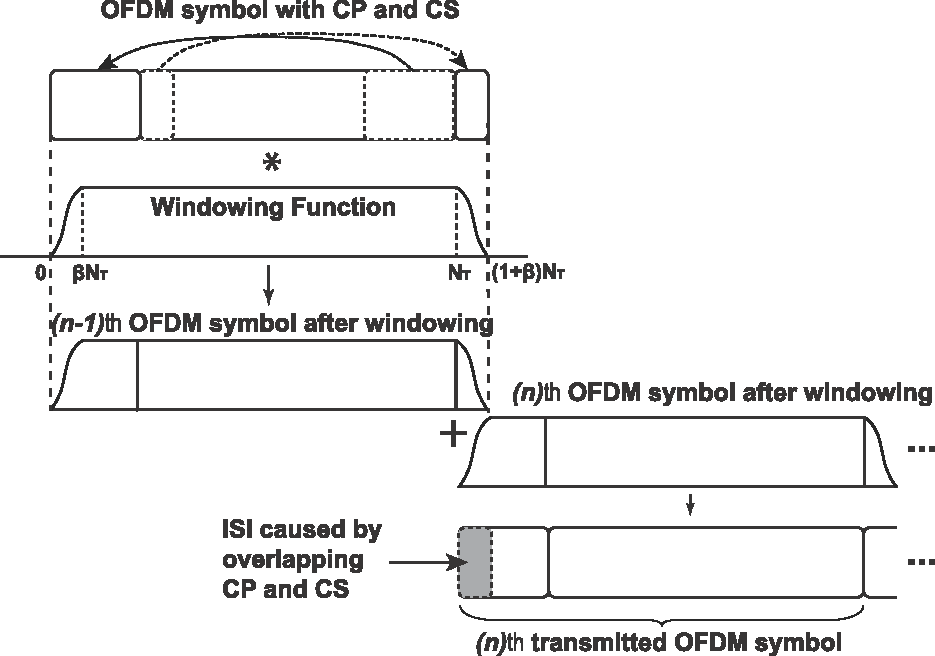
\includegraphics [width=0.9\columnwidth, height=7.5cm] {Figures/w-ofdm} }
	\vspace{-2mm}
    \caption{Pulse Shaping operation performed on OFDM symbols.}
    \label{fig:PS}
\end{figure}


\begin{figure}
	\centering
	\scalebox{1}{
	\begin{tikzpicture}
	\begin{axis}[ xlabel=Frequency (MHz), ylabel= Amplitude (dB), legend columns=3,	legend style={at={(0.5,1.02)}, anchor=south, cells={anchor=west}, draw=none}, xmin=-10, xmax=10,
	x post scale=1.4]
		\addplot+[style={dashed, color=blue}, every mark/.append style={mark=none}] coordinates
						{(-40,-50) (-15,-50) (-10,-40) (-5.5,-32) (-5,-26) (-4.5,0) (4.5,0) (5,-26) (5.5,-32) (10,-40) (15,-50) (40,-50)};
		\addlegendentry{Class C};
		\addplot+[style={dashed, color=violet}, every mark/.append style={mark=none}] coordinates
						{(-40,-65) (-15,-65) (-10,-55) (-5.5,-45) (-5,-35) (-4.5,0) (4.5,0) (5,-35) (5.5,-45) (10,-55) (15,-65) (40,-65)};
		\addlegendentry{Class D};
		\addplot+[black, style={solid, color=gray}, every mark/.append style={mark=none}]  table [x index=0, y index=1] {./Dat/PulseshapeM10.dat};
		\addlegendentry{os};
		\addplot+[black, style={dotted, color=blue, thick}, every mark/.append style={mark=none}]	 table [x index=0, y index=2] {./Dat/PulseshapeM2.dat};
		\addlegendentry{$p_1\_\beta$1};
		\addplot+[black, style={dotted, color=violet, thick}, every mark/.append style={mark=none}]  table [x index=0, y index=3] {./Dat/PulseshapeM2.dat};
		\addlegendentry{$p_2\_\beta$1};
		\addplot+[black, style={dotted,  color=red, thick}, every mark/.append style={mark=none}]	 table [x index=0, y index=4] {./Dat/PulseshapeM2.dat};
		\addlegendentry{$p_3\_\beta$1};
		\addplot+[black, style={solid, color=blue, thin}, every mark/.append style={mark=none}]	 table [x index=0, y index=2] {./Dat/PulseshapeM10.dat};
		\addlegendentry{$p_1\_\beta$5};
		\addplot+[black, style={solid, color=violet, thin}, every mark/.append style={mark=none}]  table [x index=0, y index=3] {./Dat/PulseshapeM10.dat};
		\addlegendentry{$p_2\_\beta$5};
		\addplot+[black, style={solid, color=red, thin}, every mark/.append style={mark=none}]	 table [x index=0, y index=4] {./Dat/PulseshapeM10.dat};
		\addlegendentry{$p_3\_\beta$5};
	\end{axis}
%	\end{semilogyaxis}
	\end{tikzpicture}
	}
\caption{Spectral envelope due to pulse shaping OFDM symbols using three smoothing functions and different roll-off factors for 802.11p. Class C and D spectral emission mask limits are overlaid as dotted lines.}
\label{fig:Spec_PS}
\vspace{-4mm}
\end{figure}
%
In Fig.~\ref{fig:Spec_PS}, \emph{os} shows the original OFDM spectrum without applying pulse shaping.
$p_1\_\beta1$, $p_2\_\beta1$, $p_3\_\beta1$ show the spectra of the OFDM signal using smoothing functions $p_1(m)$ to $p_3(m)$, respectively, and roll-off factor $\beta N_{T}=1$. Plots are also shown for the same functions with roll-of factor $\beta N_{T}=5$.
In the case of using one guard interval sample, the spectral leakage is reduced compared to the original OFDM signal, and  $p_1(m)$ obtains better results than the other two methods, however, the shaped spectra do not meet the emission requirement of class C.
When 5 CP samples are used for pulse shaping, $p_2(m)$ and $p_3(m)$ achieve a significant improvement, and in fact, $p_2\_\beta5$ satisfies class C and almost meets the requirement of class D.

Thus, we can state that, ignoring the presence of an image spectrum as noted previously, the pulse shaping method can take part of the guard interval to apply a smoothing function in order to shape the spectral leakage and nearly meet  stringent SEM requirements.

\begin{figure}
	\centering
	\scalebox{1}{
	\begin{tikzpicture}
	\begin{axis}[ xlabel=Frequency (MHz), ylabel= Amplitude (dB), legend columns=3,	legend style={at={(0.5,1.02), thick}, anchor=south, cells={anchor=west}, draw=none}, xmin=-10, xmax=10,
	x post scale=1.4]
		\addplot+[style={dashed, color=blue}, every mark/.append style={mark=none}] coordinates
						{(-40,-50) (-15,-50) (-10,-40) (-5.5,-32) (-5,-26) (-4.5,0) (4.5,0) (5,-26) (5.5,-32) (10,-40) (15,-50) (40,-50)};
		\addlegendentry{Class C};
		\addplot+[style={dashed, color=violet}, every mark/.append style={mark=none}] coordinates
						{(-40,-65) (-15,-65) (-10,-55) (-5.5,-45) (-5,-35) (-4.5,0) (4.5,0) (5,-35) (5.5,-45) (10,-55) (15,-65) (40,-65)};
		\addlegendentry{Class D};
		\addplot+[black, style={solid, color=lightgray}, every mark/.append style={mark=none}]  table [x index=0, y index=1] {./Dat/PulseshapeM10_inter.dat};
		\addlegendentry{os};
		\addplot+[black, style={solid, color=green}, every mark/.append style={mark=none}]	 table [x index=0, y index=2] {./Dat/PulseshapeM10_inter.dat};
		\addlegendentry{ps1\_$\beta$5};
		\addplot+[black, style={solid, color=red}, every mark/.append style={mark=none}]  table [x index=0, y index=3] {./Dat/PulseshapeM10_inter.dat};
		\addlegendentry{ps2\_$\beta$5};
		\addplot+[black, style={solid,  color=black}, every mark/.append style={mark=none}]	 table [x index=0, y index=4] {./Dat/PulseshapeM10_inter.dat};
		\addlegendentry{ps2\_$\beta$5};
	\end{axis}
	\end{tikzpicture}
	}
\caption{Spectrum of 802.11p OFDM symbols shaped with different window functions, with the image spectrum included.}
\label{fig:Inter_Spec_PS}
\vspace{-4mm}
\end{figure}

To investigate further, Fig.~\ref{fig:Inter_Spec_PS} plots simulation results for pulse shaped 802.11p OFDM symbols with the presence of the image spectrum included.
The image is a consequence of interpolation or DAC response.
The plot shows that pulse shaping yields a response that is similar to, but slightly better than, the original OFDM signal.
However, when the image spectrum is considered, pulse shaping clearly can not achieve meaningful adjacent channel signal compression.
In fact, the band gap between the main spectrum and the image spectrum is insufficient for pulse shaping to achieve any significant spectral leakage decay.

In a practical system, the consequence is that almost all of the side-lobe attenuation may need to be contributed by sharp and hence both high order and accurate analogue filters.
Such filters contribute design complexity, increased component count, manufacturing difficulty, and additional cost to a product.

\subsection{Image Spectrum Cancellation By FIR Filter}
\label{subsec:FIR}
The critical issue for 802.11p signals to meet the stringent mask requirements is that the frequency guards are narrow and the carrier frequency is relatively high (5.9\,GHz) compared to 802.11a.
Similarly, the 802.11af guard bands are even narrower, and the sub-channels are also much narrower.
Interpolation can be used at baseband to increase sampling frequency, and thereby expand the baseband bandwidth.
This then provides a wider frequency transition band, which is easier to fit a filter roll-off response into, however the resulting image spectra (repeats of the original baseband spectrum) must then be removed by filtering.
%, commonly implemented as an FIR filter, may be used to cancel image spectra.
Such filters are commonly implemented using finite impulse response (FIR) form.
A cascaded integrator comb (CIC) implementation is sometimes chosen, since this can combine the interpolation and filtering steps, however while it is computationally efficient it lacks flexibility,
Since this chapter is concerned with the tradeoff between the filter order, duration of impulse response, degree of oversampling, and filter transition band sharpness, flexibility is important and thus general FIR form filters are assumed.

The tradeoff mentioned above exists because the narrow band gap between main and adjacent image spectra mandates a high order filter to remove ICI, which generally implies a high order and thus long impulse response filter.
Unfortunately the long impulse response of the filter has a similar effect to the impulse response of the overall channel in terms of inducing ISI.
Thus the FIR filter also reduces the effective guard interval of OFDM symbols~\cite{farhang2008signal}.
Consequently, its design must contribute to the wider tradeoff between ISI avoidance, spectral efficiency (the transition band width), and degree of filter attenuation needed to meet the SEM requirement.

Several widely used FIR implementation filters are listed in Table~\ref{tab:lengthFIR}. These are all be investigated for image spectrum attenuation, as applied to 802.11p symbols initially, and then evaluated for 802.11af.
%The table lists their attenuation, and length (in taps) in the first two columns.
An empirical formula~\cite{Kapadia2012} is used to estimate the length of each filter in terms of attenuation $A$ and transition band $\Delta\omega$.
The specifications of the stringent 802.11p class D SEM are used to calculate the required number of taps with L-fold interpolation, in terms of L.

\begin{table}[h]
	\centering
	\caption{Popular window-based FIR filter lengths}
	\label{tab:lengthFIR}
	\renewcommand{\arraystretch}{1.5}
	\begin{tabular}{@{}lp{2cm}p{3.4cm}p{2.5cm}@{}}
       \toprule
    		  Window 	& Stopband Attenuation  & Filter Length, N   & Length for 802.11p\\
    	\midrule
		Hamming, 	$HM$		& $-26.5$dB	& $\frac{6.22\pi}{\Delta\omega}$							&  $N \approx 31 L$ \\
		Hanning, $HN$				& $-31.5$dB	& $\frac{6.65\pi}{\Delta\omega}$							&  $N \approx 33 L$ \\
		Backman, $BM$			& $-42.7$dB	& $\frac{11.1\pi}{\Delta\omega}$							&  $N \approx 55 L$ \\
[1ex]		Kaiser, $KS$				& --- 		&\parbox{3cm}{	$\frac{A-7.95}{2.23 \Delta\omega}, A>21$ \\
[1ex]												$\frac{5.79}{\Delta\omega}, A<21$}			& $N \approx 33 L$ \\
[1ex]		Chebyshev, $CW$		      & ---		& $\frac{2.06A -16.5}{2.29 \Delta\omega}$					& $N \approx 67 L$ \\
    	\bottomrule
    \end{tabular}
\end{table}

It is noticeable that the required lengths of these FIR filters for 802.11p are all longer than the 1.6\,us guard interval of the 802.11p symbol.
For example, the Hanning window requires filter length $N \approx 33\times L$ samples (each sample duration is $\frac{1}{L.10MHz}$ ), equivalent to a duration of 3.3~us.
%Thinh: I added "1.6us" above... is that correct? How did you compute the filter time in us? Is this example correct: if N=33L and each sample duration is L/10MHz then the duration is 3.3us}
To avoid ISI, the maximum length of the FIR filter is derived by taking into account the guard interval and the CIR.
By assuming that the delay spread of the vehicular channel is constrained to a maximum of 600~ns (as discussed in Section~\ref{sec:SigMod}) based on the results stated in \cite{Acosta-Marum2007,Sen2008}, the CIR is equivalent to 6 samples of the 802.11p guard interval (the sampling frequency of 802.11p is 10\,MHz).
Therefore, a remaining effective guard interval of 10 samples is available for filtering.
However, when the filter is used in a transmitter, a matched filter is required at the receiver~\cite{farhang2008signal} with equivalent length, meaning that the remaining guard interval is effectively halved: only 5 samples remain for transmitter filtering.

Given that L-fold interpolation is used at the transmitter, the permitted FIR filter length becomes $5 \times L$, constituting one of the rules for the FIR filter design process.

Theoretically, in the conventional approach, a value of $L$ can be chosen based on the baseband sampling frequency ($F_s=$10\,MHz for 802.11p) and the DAC maximum frequency, $F_{DAC}^{max}$, such that $F_{DAC}=L.F_s \le F_{DAC}^{max}$.

In the proposed method, the baseband frequency of the OFDM symbol is increased by a factor of $M$ over the critical sampling frequency (where $M$ is a power of two). Thus, to maintain the same DAC sampling frequency, $F_{DAC}=L'\cdot M\cdot Fs$, only $L'$-fold interpolation is required.
It is clearly preferable that $L'/M$ is an integer.
For comparison between the proposed and conventional approaches, $L$ should also be an integer, and in this chapter, assuming $F_{DAC}^{max}$=80\,MHz, we choose $L=8$ for the conventional method, and compare with two values of $L'$ ($2$ and $4$).

\begin{figure}
	\centering
	\scalebox{1}{
	\begin{tikzpicture}
	\begin{axis}[ xlabel=Frequency (MHz), ylabel= Amplitude (dB), legend columns=4,	legend style={at={(0.5,1.02, ultra thick)}, anchor=south, cells={anchor=west}, draw=none}, xmin=-20, xmax=20,
	x post scale=1.4]

		\addplot+[style={dashed, color=black}, every mark/.append style={mark=none}] coordinates
						{(-40,-40) (-15,-40) (-10,-28) (-5.5,-20) (-5,-10) (-4.5,0) (4.5,0) (5,-10) (5.5,-20) (10,-28) (15,-40) (40,-40)};
		\addlegendentry{Class A};
		\addplot+[style={dashed, color=green}, every mark/.append style={mark=none}] coordinates
						{(-40,-40) (-15,-40) (-10,-28) (-5.5,-20) (-5,-16) (-4.5,0) (4.5,0) (5,-16) (5.5,-20) (10,-28) (15,-40) (40,-40)};
		\addlegendentry{Class B};
		\addplot+[style={dashed, color=blue}, every mark/.append style={mark=none}] coordinates
						{(-40,-50) (-15,-50) (-10,-40) (-5.5,-32) (-5,-26) (-4.5,0) (4.5,0) (5,-26) (5.5,-32) (10,-40) (15,-50) (40,-50)};
		\addlegendentry{Class C};
		\addplot+[style={dashed, color=violet}, every mark/.append style={mark=none}] coordinates
						{(-40,-65) (-15,-65) (-10,-55) (-5.5,-45) (-5,-35) (-4.5,0) (4.5,0) (5,-35) (5.5,-45) (10,-55) (15,-65) (40,-65)};
		\addlegendentry{Class D};

		\addplot+[smooth, style={solid, color=green, thin}, every mark/.append style={mark=none}]	 table [x index=0, y index=2] {./Dat/filtered_spec.dat};
		\addlegendentry{KS};
		\addplot+[smooth, style={solid, color=cyan, thin}, every mark/.append style={mark=none}]  table [x index=0, y index=3] {./Dat/filtered_spec.dat};
		\addlegendentry{HM};
		\addplot+[smooth, style={solid, color=red, thin}, every mark/.append style={mark=none}]	 table [x index=0, y index=4] {./Dat/filtered_spec.dat};
		\addlegendentry{HN};
		\addplot+[smooth, style={solid, color=blue, thin}, every mark/.append style={mark=none}]	 table [x index=0, y index=5] {./Dat/filtered_spec.dat};
		\addlegendentry{BM};
		\addplot+[smooth, style={solid, color=black, thin}, every mark/.append style={mark=none}]	 table [x index=0, y index=7] {./Dat/filtered_spec.dat};
		\addlegendentry{CW};
	\end{axis}
	\end{tikzpicture}
	}
	\vspace{-2mm}
\caption{Spectra of OFDM symbols for 802.11p using different FIR interpolation filters, with $L=8$.}
\label{fig:FirSpec}
\vspace{-4mm}
\end{figure}

To visualise the spectral performance, a simulation is performed, with $L=8$, to evaluate filtered spectra using each window function, for 802.11p symbols.
The spectral responses are plotted in Fig.~\ref{fig:FirSpec}, where the same OFDM signal as in Fig.~\ref{fig:Inter_Spec_PS} has been filtered by the FIR interpolation filters, and compared to the SEMs.
In the figure, the filtered spectra obtained by using Kaiser, Hamming, Hanning, Blackman, and Chebyshev windows are compared (denoted using the abbreviations in Table~\ref{tab:lengthFIR}).
In each case, two prominent auxiliary peaks, visible beside the main spectrum, are the biggest impediments to satisfying the SEM criteria.
In detail, the Blackman filtered spectrum slightly exceeds the class A limits, whereas the remaining filters are able to meet the requirements of classes A and B but not of classes C and D. In fact, none of the filters are even close to class C and D compliance.
Hence, given the effective guard interval of 802.11p, FIR filtering clearly does not provide a solution.

The simulation results show that the common filtering methods used at interpolated baseband are not even close to meeting the strict SEM requirements of 802.11p.
Although not shown here, this is of course equally true of the more stringent 802.11af SEM.
This result implies that 802.11p and 802.11af implementations must rely on sharp front end RF and analogue filtering, which typically results in an increased total system cost and reduced power efficiency.

%---------------------------------------------------------------------------------
\section{A Spectrum Efficient Shaping Method}
%---------------------------------------------------------------------------------
The discussions above have revealed that the main challenge to conforming with strict SEMs is the narrow frequency guard which must accommodate a very sharp filter transition between pass and stop bands, since the stop-band attenuation is high.
In this section, we briefly explain the method before building upon its foundation to derive a CR architecture for OFDM spectral leakage mitigation which we will then evaluate for both 802.11p and 802.11af.

\subsection{New Spectral Leakage Filtering Method}

In a conventional approach, pulse shaping is only employed with small roll-off factors.
This is because large roll-off factors involve longer filters, reducing the effective guard interval.
Given the narrow frequency guard of the OFDM spectrum for the new standards, and the amount left after accounting for the effects of CIR and matching filters, pulse shaping under such constraints is unable to cancel the image spectrum: in fact, even if the entire guard interval was to be used, this may be insufficient for the very stringent class D SEM in 802.11p, and the SEM of 802.11af.
Thus our new method takes a different approach.
Instead of using a large proportion of the guard interval for FIR filtering, we allow the pulse shaping to occupy a significant portion of the guard space, with large roll-off factors.
To obtain the significant spectral leakage reduction necessary, the frequency guard needs to be increased.
It thus involves introducing a frequency guard extension technique.
Then, given a wider frequency guard, pulse shaping with large roll-off factors can achieve significant side lobe compression of the OFDM signal, and the required transition band for FIR filtering is extended, which means a shorter FIR filter is able to attenuate the image spectrum.

The method thus involves three steps:

\begin{itemize}
\item The IFFT length is multiplied by a factor $M$, and the sampling frequency similarly increased by a factor $M$, to maintain the same subcarrier spacing.
Given this, the allocation vector is formed to add data symbols at lower sub-carriers that are the same as those in the original IFFT, while the remaining sub-carriers are zero-padded.
\item Next, pulse shaping is applied in the normal way, to meet the given SEM constraint.
\item Finally, $L'$-fold interpolation is used to allow simple filtering to remove the image spectrum.
\end{itemize}

Based on the proposed approach, we build a flexible CR architecture which is demonstrated to achieve the SEM requirements for both 802.11p (all classes A, B, C and D) as well as 802.11af in the UHF band.

\subsection{Novel CR Filtering Architecture}

A CR architecture for OFDM implies the agility to handle non-contiguous (NC) transmission of symbols (NC-OFDM) as well as the ability to adapt to different frequency bands, bandwidths and timing synchronisation regimes.
For the purposes of this chapter, a CR architecture is developed which combines  transmission of NC-OFDM symbols with switched sampling frequency, supporting both 802.11p and 802.11af.
In particular, the architecture adaptively extends the frequency guard as required, and performs both pulse shaping and FIR interpolation filtering to meet the most strict SEM requirements of both standards.
It should be understood that this CR architecture is designed to demonstrate compliance with the more difficult standards: it could trivially be de-rated to the much less stringent 802.11a and 802.11ac parent standards.

The proposed CR-based transmitter architecture structure is presented in Fig.~\ref{fig:Struc}, as implemented on a Xilinx FPGA for experimental purposes.
\begin{figure}[t]
    \centerline{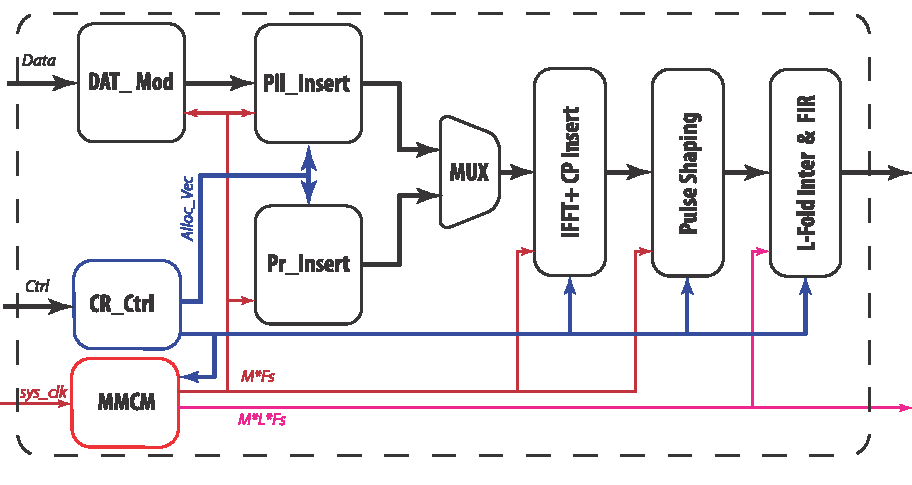
\includegraphics [width=0.9\columnwidth] {Figures/CRTx_shaping} }
	\vspace{-2mm}
    \caption{The CR-Based architecture for adaptive OFDM spectral leakage shaping.}
    \label{fig:Struc}
\end{figure}
As can be seen, the architecture consists of the baseband sub-modules, including %data modulation ($DAT_Mod$), pilot insertion ($Pil_Insert$), preamble insertion ($Pr_Insert$), IFFT and CP adding ($IFFT+CP insert$), $Pulse shaping$, L-fold interpolation and FIR filtering ($L-Fold Inter \& FIR$).
\emph{Pil\_Insert} which flexibly inserts data symbols and pilots from the data modulator, \emph{DAT\_Mod}, into an OFDM symbol according to the current allocation vector (\emph{Alloc\_Vec}).
\emph{Pre\_Insert} inserts the preamble symbol while \emph{IFFT+CP Insert} is an IP core that with flexibly reconfigurable IFFT length and CP insertion.
\emph{PulseShaping} performs pulse shaping with a smoothing function for which the roll-off factor can be changed from small, for relaxed spectral shaping, to large, for more stringent spectral shaping.
\emph{L-Fold Inter\&FIR} performs $L'$-fold interpolation, with $L'$ being controllable on a symbol-by-symbol basis. After interpolation, the FIR block is used to filter out the image spectrum.
In addition, for the CR architecture, the cognitive control sub-module (\emph{CR\_Ctrl}) is used to modify sub-module parameters to match SEM requirements imposed from the higher layers (i.e.\ it adjusts timing, bandwidth, frequency band and SEM requirements).
The mixed-mode clock manager (\emph{MMCM}) is another integrated IP core used to manage the sampling clock ($\mathit{F_s}$), which is set according to the filter performance requirements and operating frequency band.

In addition, the \emph{MMCM} allows the transmitter to reduce the degree of filtering (i.e. degree of spectral leakage shaping) when transmission power is reduced: since transmit power reduction naturally reduces ICI.
This is particularly important for lower power operating modes in which a lower sampling frequency, less filtering complexity, and reduced transmission amplitude all contribute to power savings.

Compare this with the 802.11p prototype presented in \cite{Choi2014}, which was adopted for direct device-to-device communication between smartphones.
That innovative prototype was able to adaptively increase transmission power to extend communication range.
However, the system was based on an 802.11a hardware solution and baseband, and did not investigate the increased spectral leakage when the transmitted signal was amplified to increase range (at which point it would not be likely to meet the 802.11p SEM requirement).

By contrast, the method proposed and implemented in this chapter, is able to apply a more stringent SEM filter when transmission power is increased such that ICI exceeds a given threshold.
In particular, \emph{CR\_Ctrl} is invoked to change the IFFT length to $M$ times the original IFFT, while \emph{Alloc\_Vec} extends the frequency guard and \emph{MMCM} increases $\mathit{F_s}$ according to the required IFFT length.
Moreover, \emph{CR\_Ctrl} changes \emph{PulseShaping} to use a large roll-off factor, reduces the $L$-fold interpolation (since $L'\times M$ is constant) and shortens the FIR length to meet the more stringent SEMs.
On the other hand, when a device and access point are in closer proximity, the transmission power can be reduced such that the spectral leakage is small, and thus filtering can be relaxed.
In this case, \emph{CR\_Ctrl} is invoked to change the IFFT length back to the original, and employ \emph{PulseShaping} with a small roll-off factor. Moreover, \emph{L-Fold Inter\&FIR} switches back to a normal range in order to reduce the amount of computation.
It should be noted that the additional computation needed for signal processing in the baseband (which uses low cost, low power components), can be more than compensated for by relaxing the specification of the RF front-end design since the analogue filtering requirements are so much less strict.

The following Section presents the application of the proposed CR architecture in performing stringent filtering to achieve the SEM specifications of both 802.11p and 802.11af respectively.

%---------------------------------------------------------------------------------
\section{Simulation Results and Discussion}
%---------------------------------------------------------------------------------
\subsection{Configuration and Performance Evaluation for 802.11p}
Based on the signal model and environmental factors discussed in Section~\ref{sec:SigMod}, the CIR length is assumed to not exceed 60\,~ns.
Therefore, the effective guard interval, equivalent to the length of 10 samples of the original CP, i.e., $10 \times 100=1000$\,ns, is used for the pulse shaping and FIR filter.
By choosing a DAC sampling frequency of 80\,MHz, the sampling frequency for 802.11p is increased by 8 times ($L'.M = 8$) over the original nominal rate of 10~MHz.
Based on this configuration, two optional systems, denoted as \emph{Prop1} and \emph{Prop2}, will now be explored for 802.11p:

\emph{Prop1} doubles the size of the IFFT, i.e., $M=2$, which means doubling the sampling frequency to extend the frequency guard, after which 4-fold interpolation, i.e., $L'=4$, is required to obtain a sampling frequency of 80\,MHz.

\emph{Prop2} quadruples the size of the IFFT, i.e., $M=4$; Then applies 2-fold interpolation, i.e., $L'=2$ to achieve the 80\,MHz sampling frequency.

Based on the results in subsection~\ref{subsec:Pulse}, $p_2(m)$ is employed with $\beta N_{T}=5 \times M$. i.e.\ equivalent to the length of 5 samples of the original CP, i.e., 500\,ns.
It should be noted that, after extending the frequency guard, the number of samples in the symbol, including CP, is increased $M$ times.
Fig.~\ref{fig:OverSpec} plots the shaped spectrum of the proposed method after interpolation in the baseband, at a sample frequency of 80\,MHz.
The original spectrum denoted \emph{Conv}, and the specifications for classes C and D are also shown.
The main spectrum of \emph{Prop1} and \emph{Prop2} almost satisfy class D.
The image spectrum of \emph{Prop1} is present at $\pm$20\,MHz and $\pm$40\,MHz whereas \emph{Prop2} has an image spectrum at $\pm$40\,MHz only.

\begin{figure}
	\centering
	\scalebox{1}{
	\begin{tikzpicture}
	\begin{axis}[ xlabel=Frequency (MHz), ylabel= Amplitude(dB), legend columns=4,	legend style={at={(0.5,1.02)}, anchor=south, cells={anchor=west}, draw=none}, xmin=-40, xmax=40,
	x post scale=1.4]
		\addplot+[style={dashed, color=blue}, every mark/.append style={mark=none}] coordinates
						{(-40,-50) (-15,-50) (-10,-40) (-5.5,-32) (-5,-26) (-4.5,0) (4.5,0) (5,-26) (5.5,-32) (10,-40) (15,-50) (40,-50)};
		\addlegendentry{Class C};
		\addplot+[style={dashed, color=violet}, every mark/.append style={mark=none}] coordinates
						{(-40,-65) (-15,-65) (-10,-55) (-5.5,-45) (-5,-35) (-4.5,0) (4.5,0) (5,-35) (5.5,-45) (10,-55) (15,-65) (40,-65)};
		\addlegendentry{Class D};
		\addplot+[black, style={solid, color=green}, every mark/.append style={mark=none}]  table [x index=0, y index=1] {./Dat/OverSpec.dat};
		\addlegendentry{Conv};
		\addplot+[black, style={solid, color=red}, every mark/.append style={mark=none}]	 table [x index=0, y index=2] {./Dat/OverSpec.dat};
		\addlegendentry{Prop1};
		\addplot+[black, style={solid, color=blue}, every mark/.append style={mark=none}]  table [x index=0, y index=3] {./Dat/OverSpec.dat};
		\addlegendentry{Prop2};
%		\addplot+[black, style={solid,  color=black, thin}, every mark/.append style={mark=none}] table [x index=0, y index=4] {./Dat/OverSpec.dat};
%		\addlegendentry{HN};
	\end{axis}
	\end{tikzpicture}
	}
	\vspace{-2mm}
\caption{Spectrum of 802.11p signal of the proposed CR architecture after interpolation.}
\label{fig:OverSpec}
\end{figure}

A simpler, shorter-length FIR filter is needed to cancel the image spectra, since they lie much further away in frequency than for the original approach, \emph{Conv}.
The remaining guard interval for the transmitter filter and matched filter is 500\,ns.
Therefore, the maximum impulse response available for the image rejection FIR filter is 250\,ns, which is equivalent to $2.5 \times M.L'$ samples at the 80\,MHz sampling frequency.

FIR filters are designed for \emph{Prop1} and \emph{Prop2} respectively, using a Kaiser window. For \emph{Prop1}, since the frequency guard is still relatively narrow, an FIR filter with an impulse length of 20 samples is required to cancel the image spectrum.
Fig.~\ref{fig:OptSpec1} shows the result of spectrum filtering for \emph{Prop1}, with the original OFDM spectrum (\emph{Conv}) and SEMs for classes C and D overlaid.
It can be seen that there are still two small peaks caused by the image spectrum, but these are compressed by the FIR filter to meet the class D requirement.
Some distortion is noticeable in the main spectrum due to the effects of the FIR filter.

\emph{Prop2} has a wider frequency guard compared to \emph{Prop1} and thus its FIR filter only requires a length of 12 samples to cancel the image spectrum. A remaining effective guard interval of 200\,ns is reserved.
Fig.~\ref{fig:OptSpec2} plots the result of this degree of spectral filtering for \emph{Prop2} and with respect to the class C and D SEMs.
Clearly the image spectrum of \emph{Prop2} can be cancelled by a short-length FIR filter, while suffering less distortion (rounding) to the main passband.
%whilst that for $\mathit{Prop}1$ still remains too large in magnitude.
%Hence, $\mathit{Prop}2$ meets the class D specification.

\begin{figure}
	\centering
	\scalebox{1}{
	\begin{tikzpicture}
	\begin{axis}[ xlabel=Frequency (MHz), ylabel= Amplitude (dB), legend columns=4,	legend style={at={(0.5,1.02, ultra thick)}, anchor=south, cells={anchor=west}, draw=none}, xmin=-40, xmax=40,
	x post scale=1.4]
		\addplot+[style={dashed, color=blue}, every mark/.append style={mark=none}] coordinates
						{(-40,-50) (-15,-50) (-10,-40) (-5.5,-32) (-5,-26) (-4.5,0) (4.5,0) (5,-26) (5.5,-32) (10,-40) (15,-50) (40,-50)};
		\addlegendentry{Class C};
		\addplot+[style={dashed, color=violet}, every mark/.append style={mark=none}] coordinates
						{(-40,-65) (-15,-65) (-10,-55) (-5.5,-45) (-5,-35) (-4.5,0) (4.5,0) (5,-35) (5.5,-45) (10,-55) (15,-65) (40,-65)};
		\addlegendentry{Class D};
		\addplot+[smooth, style={solid, color=green}, every mark/.append style={mark=none}]  table [x index=0, y index=1] {./Dat/OptSpec1.dat};
		\addlegendentry{Conv};
		\addplot+[smooth, style={solid, color=red, thick}, every mark/.append style={mark=none}]	 table [x index=0, y index=2] {./Dat/OptSpec1.dat};
		\addlegendentry{Prop1};
%		\addplot+[smooth, style={densely dashed, color=blue, very thin}, every mark/.append style={mark=none}]  table [x index=0, y index=3] {./Dat/OptSpec1.dat};
%		\addlegendentry{OPT2};
%		\addplot+[smooth, style={solid, color=black, very thin}, every mark/.append style={mark=none}]	 table [x index=0, y index=4] {./Dat/OptSpec1.dat};
%		\addlegendentry{HN};
	\end{axis}
	\end{tikzpicture}
	}
	\vspace{-2mm}
\caption{Spectrum of 802.11p signal using option \emph{Prop1} with 20th order FIR filtering.}
\label{fig:OptSpec1}
\end{figure}

\begin{figure}
	\centering
	\scalebox{1}{
	\begin{tikzpicture}
	\begin{axis}[ xlabel=Frequency (MHz), ylabel= Amplitude (dB), legend columns=4,	legend style={at={(0.5,1.02, ultra thick)}, anchor=south, cells={anchor=west}, draw=none}, xmin=-40, xmax=40,
	x post scale=1.4]
		\addplot+[style={dashed, color=blue}, every mark/.append style={mark=none}] coordinates
						{(-40,-50) (-15,-50) (-10,-40) (-5.5,-32) (-5,-26) (-4.5,0) (4.5,0) (5,-26) (5.5,-32) (10,-40) (15,-50) (40,-50)};
		\addlegendentry{Class C};
		\addplot+[style={dashed, color=violet}, every mark/.append style={mark=none}] coordinates
						{(-40,-65) (-15,-65) (-10,-55) (-5.5,-45) (-5,-35) (-4.5,0) (4.5,0) (5,-35) (5.5,-45) (10,-55) (15,-65) (40,-65)};
		\addlegendentry{Class D};
		\addplot+[smooth, style={solid, color=green}, every mark/.append style={mark=none}]  table [x index=0, y index=1] {./Dat/OptSpec2.dat};
		\addlegendentry{Conv};
%%IVM		\addplot+[smooth, style={densely dashed, color=red, very thin}, every mark/.append style={mark=none}]	 table [x index=0, y index=2] {./Dat/OptSpec2.dat};
%%IVM		\addlegendentry{Prop1};
		\addplot+[smooth, style={solid, color=blue, thick}, every mark/.append style={mark=none}]  table [x index=0, y index=3] {./Dat/OptSpec2.dat};
		\addlegendentry{Prop2};
%		\addplot+[smooth, style={solid, color=black, very thin}, every mark/.append style={mark=none}]	 table [x index=0, y index=4] {./Dat/OptSpec2.dat};
%		\addlegendentry{HN};
	\end{axis}
	\end{tikzpicture}
	}
	\vspace{-2mm}
\caption{Spectrum of 802.11p signal for \emph{Prop2} with 12th order FIR filtering.}
\label{fig:OptSpec2}
\end{figure}

Overall, the simulation results demonstrate that the proposed CR architecture can  meet the specification of class D, the most stringent of the four 802.11p SEMs.
\emph{Prop2} obtains better performance in terms of distortion and effective guard interval compared to \emph{Prop1}, but pays the cost of a higher computational requirement due to the increased IFFT size.

\subsection{Configuration and Performance Evaluation for 802.11af}

Based on the discussion in Section~\ref{sec:SigMod}, if the CIR length is assumed to not exceed 1\,us, this is equivalent to 6 samples in the 802.11af CP.
Therefore, the effective guard interval, equivalent to a length of 26 samples of the original CP, is available for use by the pulse shaping and FIR filters.

By choosing a DAC sampling frequency of 48\,MHz, the output sampling frequency of 802.11af is increased by 8 times ($L'.M =8$) compared to the original nominal frequency (6\,MHz).
Simulation results for shaping the spectral leakage of 802.11af are presented here.
The proposed method is compared to the conventional approach which make use of state-of-the-art pulse shaping and FIR filtering.
In the conventional approach, pulse shaping uses 2 samples in the CP for a smoothing function, and the length of the FIR filter for cancelling the image spectrum is allowed to extend to 96 ($\frac{26-2}{2} \times 8$) to avoid ISI.
Again, the FIR filter is designed using a Kaiser window, with a cut-off frequency set to attempt to compress the signal spectrum to meet the FCC mandated SEM.

Our proposed method quadruples the size of the IFFT (i.e. $M=4$), to extend the frequency guard.
Pulse shaping is configured to employ $p_2(m)$ from Subsection~\ref{subsec:Pulse}, with $\beta N_{T}=20 \times M$. That is equivalent to the length of 20 samples of the original CP.
Then 2-fold interpolation (i.e. $L'=2$), is required to obtain the sampling frequency of 48\,MHz.
The maximum allowed FIR filter length for cancelling the image spectrum without inducing ISI is equivalent to 3 samples of the original CP.
Fig.~\ref{fig:80211af} illustrates the results of shaping the spectral leakage for 802.11af using this proposed CR architecture.

\begin{figure}
	\centering
	\scalebox{1}{
	\begin{tikzpicture}
	\begin{axis}[ xlabel=Frequency (MHz), ylabel= Amplitude (dB), legend columns=4,	legend style={at={(0.5,1.02, ultra thick)}, anchor=south, cells={anchor=west}, draw=none}, xmin=-9, xmax=9,
	x post scale=1.4]
		\addplot+[style={dashed, color=violet}, every mark/.append style={mark=none}] coordinates
						{(-24,-69) (-21,-69) (-15,-53) (-9,-53) (-8.99,-55) (-3.1,-55) (-3,0) (3,0) (3.1,-55) (8.99,-55) (9,-53) (15,-53) (21,-69) (24,-69)};
		\addlegendentry{802.11af SEM};
		\addplot+[smooth, style={solid, color=red}, every mark/.append style={mark=none}]  table [x index=0, y index=1] {./Dat/80211af.dat};
		\addlegendentry{Conv};
		\addplot+[smooth, style={solid, color=blue,thick}, every mark/.append style={mark=none}] table [x index=0, y index=2] {./Dat/80211af.dat};
		\addlegendentry{Prop};

	\end{axis}
	\end{tikzpicture}
	}
	\vspace{-2mm}
\caption{Spectrum of 802.11af signal using the proposed CR architecture.}
\label{fig:80211af}
\end{figure}
%
Because of the limited length, the band transition of the FIR filter is not narrow enough.
This results in the spectrum of the conventional method, \emph{Conv}, exhibiting two side lobes, as well as introducing visible distortion in the main spectrum.
Thus, the conventional method is far from able to meet the SEM requirement for 802.11af.
One method that might be considered for achieving this is to deactivate the outer sub-carriers (instead, use null-subcarriers).
This can extend the frequency guard, but clearly results in a loss of spectral efficiency.
Reducing transmission power is also possible, but is similarly unattractive since it would adversely impact range -- in fact the power reduction needed to bring the \emph{Conv} transmission within the SEM envelope is not small.
For example, the 802.11af prototype hardware in \cite{Lan2013} requires the transmitted power to be attenuated by 20dB to satisfy the SEM specifications.

On the other hand, the spectrum of the proposed CR architecture, denoted in Fig. ~\ref{fig:80211af} as \emph{Prop}, comfortably meets the SEM specification without impacting either range or spectral efficiency.

\subsection{802.11af Spectral Efficiency}

Another way of investigating performance is to compute spectral efficiency, given a flexible allocation of subcarriers.
In other words to adjust the number of occupied subcarriers until the transmission profile fits within the 802.11af SEM, and using the unoccupied subcarrier space for filter roll off.
In the conventional method (Fig. ~\ref{fig:80211af}), about 35~dBc additional filtering would be needed to suppress the image spectrum at the edge of the channel bandwidth (3\,MHz), from -20\,dBc, to -55\,dBc.

With a 96th order FIR filter as mentioned above for \emph{Conv}, the transition band needed to achieve such suppression is estimated, based on the Kaiser window formula in Table~\ref{tab:lengthFIR}, as being 0.83\,MHz.
This is equivalent to 21 subcarrier spacings which would need to be trimmed from each side of the 802.11af channel.
Thus the number of occupied sub-carriers would need to be reduced from the standard 114 subcarriers to below 100 in order to give \emph{Conv} a sufficient guard interval for FIR filtering.

However, the window formula is only an estimate, and hence the system is simulated here to explore further.
In this case, the number of sub-carriers is reduced step-wise in pairs, from the edges working inwards, until the SEM is just satisfied.
Fig.~\ref{fig:80211af2} plots results with 94 and 92 sub-carriers occupied (\emph{Conv\_92s} and \emph{Conv\_92s}), showing that 92 sub-carriers meets the SEM requirement whereas 94 sub-carriers does not, by a small margin.

Referring back to Fig.~\ref{fig:80211af}, we also see a clear frequency gap between the spectrum of the proposed approach and the SEM.
This gap could potentially be exploited to pack in several more occupied sub-carriers.
We therefore undertake simulations to explore this phenomenon, and find that the proposed method is able to pack in up to 124 employed sub-carriers while still satisfying the SEM.
This is also illustrated in Fig.~\ref{fig:80211af2} as \emph{Prop\_124s}.

The results demonstrate that the proposed CR architecture can not only meet the stringent SEM requirement of 802.11af but could also be used to enhance spectral efficiency beyond that.
Compared to the approach of trimming off edge carriers needed by an equivalent transmission power conventional system in order to satisfy the SEM, the proposed approach to CR spectrum shaping increases spectral efficiency by 32\%.

\begin{figure}
	\centering
	\scalebox{1}{
	\begin{tikzpicture}
	\begin{axis}[ xlabel=Frequency (MHz), ylabel= Amplitude (dB), legend columns=4,	legend style={at={(0.5,1.02, ultra thick)}, anchor=south, cells={anchor=west}, draw=none}, xmin=-9, xmax=9,
	x post scale=1.4]
		\addplot+[style={dashed, color=violet}, every mark/.append style={mark=none}] coordinates
						{(-24,-69) (-21,-69) (-15,-53) (-9,-53) (-8.99,-55) (-3.1,-55) (-3,0) (3,0) (3.1,-55) (8.99,-55) (9,-53) (15,-53) (21,-69) (24,-69)};
		\addlegendentry{802.11af SEM};
		\addplot+[smooth, style={solid, color=red}, every mark/.append style={mark=none}]  table [x index=0, y index=1] {./Dat/80211af_92.dat};
		\addlegendentry{Conv\_92s};
		\addplot+[smooth, style={solid, color=green}, every mark/.append style={mark=none}]  table [x index=0, y index=1] {./Dat/80211af_94.dat};
		\addlegendentry{Conv\_94s};
		\addplot+[smooth, style={solid, color=blue, thick}, every mark/.append style={mark=none}] 	 table [x index=0, y index=2] {./Dat/80211af_124.dat};
		\addlegendentry{Prop\_124s};
	\end{axis}
	\end{tikzpicture}
	}
	\vspace{-2mm}
\caption{Fitting Filtered Spectrum of 802.11af signal to SEMs.}
\label{fig:80211af2}
\end{figure}

%---------------------------------------------------------------------------------
\section{Summary}
%---------------------------------------------------------------------------------
In this chapter, shaping the OFDM leakage spectrum has been investigated at baseband within a CR architecture, in order to meet stringent spectral emission mask (SEM) requirements.
In particular, this research considers two relatively new standards, 802.11p and 802.11af, which are defined for the physical layer and largely based upon existing standards.
In both cases, the extended physical layers are scaled to encourage reuse of existing hardware, devices and designs, but the resulting systems are then subject to much more stringent SEMs.
The research relies upon a combination of interpolation, IFFT length adjustment, pulse shaping and FIR image suppression filtering, to mitigate against spectral leakage into adjacent channels.
Simulations show that the proposed architecture can meet the specification of the four 802.11p classes A to D, as well as the stringent FCC-imposed SEM for 802.11af in the UHF
band.
The proposed method is also shown able to improve the achievable spectral efficiency for reuse of Television White Spaces in the 802.11af standard by 32\%, given equivalent transmission power, compared to conventional approaches which need to drop the outermost subcarriers in order to meet SEM requirements.
In addition, the architecture has the ability to adaptively change the degree of spectral leakage filtering in response to transmission power.
The computation of filtering can be reduced when transmission power is low, but when transmission power is high, it is able to extend to meet the strict SEM specification of both 802.11p and 802.11af.
Furthermore, the architecture is capable of adjusting clock rate, bandwidth, and frequency band on a symbol-by-symbol basis, in order to implement an agile CR solution.
%The work presented in this chapter is firstly published in [C1] and then extended to be submitted to [J4].
\chapter{A Spectrum Efficient Shaping Method}
\label{chap:SpectralLeakage}
%%!TEX root = main_thesis.tex
%---------------------------------------------------------------------------------
\chapter{An Architecture for Multi-Standard Cognitive Radios}
\label{chap:MSCR}
%---------------------------------------------------------------------------------
\definecolor{F1}{HTML}{a1dab4}
\definecolor{F2}{HTML}{225ea8}
\definecolor{F3}{HTML}{41b6c4}
%---------------------------------------------------------------------------------
\section{Introduction}
%---------------------------------------------------------------------------------
Cognitive radios that support multiple bands, multiple standards and adapt operation according to environmental conditions are becoming more attractive as the demand for higher bandwidth and more efficient spectrum use increases.
Traditional implementations in custom ASICs cannot support such flexibility, with standards changing at a faster pace, while software implementations of baseband communications fail to achieve the performance required.
Hence, FPGAs offer an ideal platform bringing together flexibility, performance, and efficiency.
In this chapter, we show how we can incorporate our contributions in previous chapters into a flexible architecture for multi-standard cognitive radios (MSCR).
We show that combining partial reconfiguration (PR) with parameterised  modules offers flexibility while minimising reconfiguration time.
To the best of our knowledge, we have not encountered work on dynamically reconfigurable OFDM baseband processing for multiple standards.

The work presented in this chapter has also been discussed in:
\begin{itemize}
\item T. H. Pham, S. A. Fahmy, and I. V. McLoughlin, ``Efficient Multi-Standard Cognitive Radios on FPGAs,'' PhD Forum Poster in \textit{Proceedings of the International Conference on Field Programmable Logic and Applications (FPL), Munich, Germany, September 2014}~\cite{Pham2014a}.
\item T. H. Pham, S. A. Fahmy, and I. V. McLoughlin, ``Efficient OFDM-based baseband processing for Multi-Standard Cognitive Radios on FPGAs,'' in preparation for submission to \emph{ACM Transactions on Embedded Computing Systems}.
\end{itemize}

%---------------------------------------------------------------------------------
\section{Related Work}
%---------------------------------------------------------------------------------
Most practical CRs are built using powerful general purpose processors to achieve flexibility through software, but they can fail to offer the computational throughput required for advanced modulation and coding techniques and they often have high power consumption.
GNU Radio~\cite{gnuradio} has been a widely used platform in academia.
It is a software application that runs on a computer or an embedded ARM processor platform, e.g. on the Ettus USRP E100.
Computational limitations mean that while it has been successful for investigating CR ideas, it is not feasible for implementing advanced embedded radios using complex algorithms.
Other software based frameworks like Iris~\cite{Sutton2010}, have some limited support for FPGAs but suffer from poor bandwidth between software and hardware.
Moreover, the compilation time and reconfiguration time of software defined radio systems can be long making them unsuitable for adapting to fast changing conditions.

In an application area with fast moving standards and requiring support for multiple standards, custom ASIC implementation is unlikely to be agile or cost effective enough to cope with fast-changing standards and operating requirements.
In order to address this, Delorme et al.~\cite{Delorme2008} presented a heterogeneous reconfigurable hardware platform for Cognitive Radio.
It can adapt its hardware structure to support standards like GSM, UMTS, and wireless LAN.
Most processing components run as embedded software on the nodes in a network-on-chip processor, while the channel coder and the mapping of the RX chain are implemented inside an FPGA.
Partial reconfiguration (PR) is used to switch the channel coder from one context to an another depending on SNR.
A processor manages data movement between the different processors, the ASIC, and the FPGA. The need for a large data buffer and inefficient data transfer mechanisms results in increased power consumption and reduced throughput.

Other platforms do not propose specific methods for managing a radio's dynamic behaviour.
KUAR~\cite{Minden2007} is a mature radio platform built around a fully-featured Pentium PC with a Xilinx Virtex II FPGA.
The baseband processing is accelerated on FPGA and limited to NC-OFDM waveforms based on the IEEE 802.16 standard.
Projects at Virginia Tech~\cite{athanaswires} have shown dynamically assembled radio structures on FPGAs, where the target radio system is defined at a high-level with datapaths connecting relatively large functional modules.
The modules are wrapped, and each of them consists of a PR module with complied partial bit-streams stored in dynamic library.
Their online assembly method eliminates the need for run time compilation, thus affording flexibility.
A flexible radio controller can insert and remove compiled modules to adapt to current conditions.
However, by using low-level reconfiguration circumventing the official PR flow, it is unclear how this approach can be mapped to newer architectures as they appear.

%---------------------------------------------------------------------------------
\section{Proposed OFDM Baseband for MSCR}
%---------------------------------------------------------------------------------
\begin{figure}
%\centering
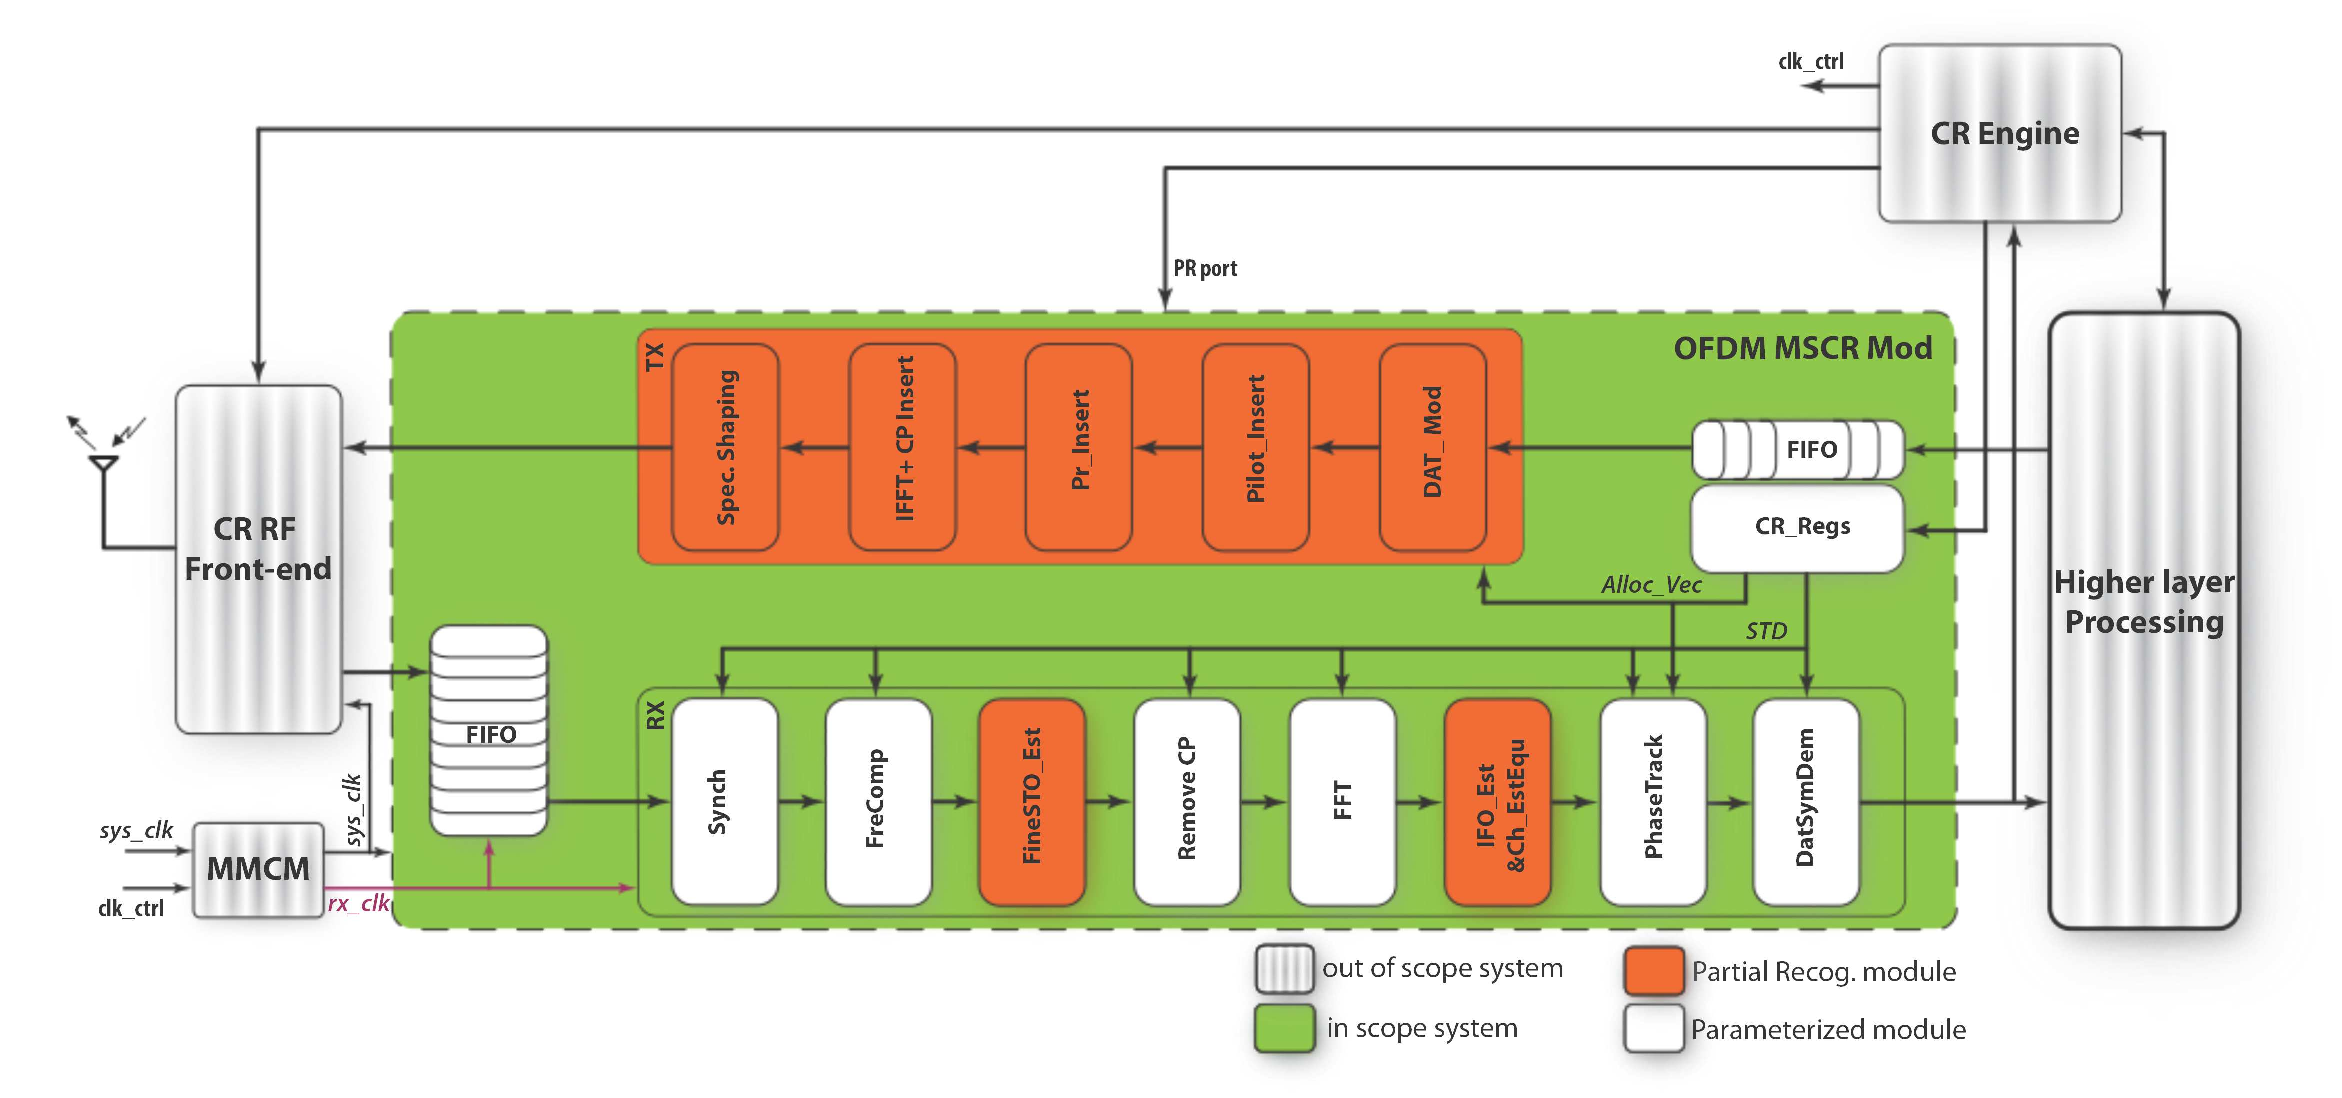
\includegraphics[width=1.05\columnwidth]{Figures/MSCRFig.eps}
\caption{The structure of a generic MSCR system}
\label{fig:struc}
\end{figure}

Fig.~\ref{fig:struc} illustrates the proposed structure of baseband modulation for our OFDM-based MSCR.
A mix of partially reconfigurable and parameterised modules make up the baseband implementation.
FIFOs are included to help overcome the reconfiguration latency when PR modules are reconfigured.
While a sink module is reconfiguring, these FIFOs store samples from the source until the module is ready to process data.
Since these modules are now just a small part of the system, buffering is significantly reduced over a more general implementation.

\subsection{System Description}

We developed a prototype MSCR baseband that supports transmitting and receiving non-contiguous OFDM (NC-OFDM) signals.
This system can perform with different OFDM symbol lengths and frame formats specified differently according to multiple standards such as IEEE~802.11~\cite{IEEE80211}, IEEE~802.16~\cite{IEEE80216}, and IEEE~802.22~\cite{IEEE80222}.
The main specifications of these standards are summarised in Table~\ref{Tab:spec}.

\begin{table}[h]
\centering
\caption{System specifications of three supported OFDM-based standards.}{
\renewcommand{\arraystretch}{1.3}
\begin{tabular}{@{}llll@{}}
\toprule
Specifications 			& IEEE~802.11 				& IEEE~802.16				& IEEE~802.22 		\\ \midrule
Frequency band			& 2.4--2.5~GHz				& 5--6~GHz					& 54--862~MHz		\\
Channel Width			& 10~MHz					& 10~MHz					& 8~MHz			\\
Sampling Frequency		& 10~MHz					& 11.52~MHz				& 9.136~Mhz		\\
FFT size ($N$)		& 64						& 256						& 2048			\\
CP Length				& 16						& 32						& 512				\\
Number of data carriers		& 48						& 192						& 1440			\\
Number of pilots			& 4						& 8						& 240				\\
\end{tabular}
\label{Tab:spec}
}
\end{table}

The CR implementation is divided into a control plane and data plane.
The data plane performs data processing on the sample data stream.
It tranceives data streams to/from the RF front end through two AXI (Advanced eXtensible Interface) stream interfaces.
For transmission, data is sent from higher layers and modulated by the data plane.
Modulated sample streams are then transferred to the RF front end to convert to analogue signals and subsequently up-converted before transmission on the RF channel.
For the receiver side, the received signals are down-converted to the baseband followed by analogue to digital conversion to form a sample stream.
The sample stream is demodulated and processed in the data plane before being transferred to a higher layer.

To support multiple standards, the data plane must provide the flexibility of switching baseband modules to the parameters specified by different standards.
AXI Stream interfaces are used for inter-module communication in the data plane as well as for communication with software.
With partial reconfiguration, modules that that swap into the same region must share the same interfaces, so this is a suitable abstraction.
The AXI Stream protocol also reduces the requirement for buffering, hence optimising resource usage and total power consumption~\cite{Liu2009}.
Each module has one slave interface to receive data from the previous module and one master interface to send processed data to the subsequent module.

The control plane is a cognitive radio (CR) engine that is required to perform adaptive based on the requirements of the application, ultimately deciding which base standard to use, and which sub-carriers to enable.
A bus register interface between the control and data planes allows them to communicate.
The CR engine also includes the PR controller that is responsible for loading bitstreams stored in DRAM into the corresponding PR regions through the ICAP (Internal Configuration Access Port) interface~\cite{Vipin2012} when necessary.

The control plane can be implemented in a number of ways.
It can be standalone software running on a processor core. It can also be hardware in a separate part of the FPGA.
Alternatively, for maximum flexibility and programming support, it can run on top of an operating system on the processor.
By ensuring that symbol data is processed and moved through the data plane independently of the processor in the control plane, we are able to achieve high throughput.
Normally, the data plane processes data streams based on a specified standard.
An allocation vector determines which sub-carriers to enable, allowing the radio to respond to varying channel occupancy conditions.
When the frequency band of the current operating mode is mostly occupied by PUs and IUs, the CR engine instructs the baseband to switch to another standard or frequency band that is currently (or will soon be) free for transmission.
The PR controller inside the CR engine is required to download the bitstreams of PR modules according to the new standard.
In the meantime, the CR engine configures the system by writing relevant parameters to registers in $CR\_Regs$ such as allocation vectors (Alloc\_vec), symbol modulation type (MOD), and standard (STD).

The scope of this chapter focuses on the managing the baseband adaptation in a way that avoids long configuration time.
We do not explore the cognitive functions, nor discuss sensing, which can be implemented in a variety of ways.
The system takes advantage of combining PR with parameterised modules to offer flexibility while minimising reconfiguration time.
The CR system is designed to be capable of operating in burst mode in which it transmits packets as soon as data is available~\cite{Ai2006}.
If a data packet is ready to be sent but reconfiguration is in progress, it is buffered in a FIFO.
It is then flushed out of FIFO for transmission after reconfiguration is completed.
Since the resource requirements for the transmitter are significantly less than the receiver, reconfiguration time is also shorter.
We discuss the resource utilisation and reconfiguration time of the transmitter in Section~\ref{sec:PerAna}.
Short reconfiguration time means there is no critical disruption of the processing chain and loss of transmitted packets.
Hence, for the transmitter, we use a single PR region with the whole transmission chain for simplicity and flexibility.

The receiver subsystem, by contrast, is required to continuously receive and process data frames.
Furthermore, the hardware usage of the receiver subsystem is much larger than the transmitter, resulting in longer reconfiguration time.
One way to avoid losing data frames, is to use a large FIFO to store received samples from the RF front end during reconfiguration, but this can be problematic as this results in significant resource usage.
Our aim here is to reduce reconfiguration time in the receive chain to mitigate the need for such large FIFOs.

We propose making some modules parameterised, while others are reconfigured using PR.
We explore how to optimise this mix in Section~\ref{sec:7module}.
Now smaller FIFOs can be used and reconfiguration can be applied at a finer granularity to minimise the impact of reconfiguration on buffer storage requirements.
After reconfiguration is complete, it is necessary to flush the FIFOs and ``catch up'' with the received samples.
This can be done by increasing the processing clock rate until the FIFOs are no longer full.
A Mixed-Mode Clock Manager (MMCM) is used for this purpose, modifying the processing clock (rec\_clk) to a higher frequency.
It is then reduced back to the sampling rate (sys\_clk) to reduce power consumption.
The MMCM module is also required to change the processing rate of data plane according to the different sampling rates specified in different standards, shown in Table~\ref{Tab:spec}.

\subsection{Module Description}\label{sec:7module}

In this section, we detail the design of each functional module shown in Fig.~\ref{fig:struc}, showing how to build a multi-standard implementation.
There is a tradeoff between the simplicity, flexibility, but long reconfiguration latency of a PR module and the increased hardware overhead, complexity, but faster configuration of a parameterised module.
The comparison between the hardware usage of parameterised modules for multiple standards and that of individual specified standard modules is evaluated.
In cases where the hardware overhead for parameterisation is a threshold of the maximum area of a stand-alone module, it is judged as better parameterised.
For those modules that require significant changes (i.e. the parameterised overhead is greater than this threshold) or are required to support unspecified parameters for future standards (such as the preamble), PR can be used on a per-module basis.
Separate bitstreams for each implementation are generated to be mapped to a PR region.
Hence, when switching the entire baseband from one standard to another, only part of the FPGA needs to be reconfigured.

\subsubsection{FIFO Buffer (FIFO)}
There are two FIFOs at the transmitter side and the receiver side to buffer data sent from the higher layer and the RF front end, respectively.
The FIFO buffers are implemented using Xilinx FIFO IP cores with 2 port AXI stream interface configuration.
In the normal operation of data stream, one data word is written to the buffer by the higher layer/the RF front end, while another one is read out from the buffer by the transmitter side/receiver side in each system clock cycle.
Therefore, the FIFOs normally operate in an almost empty state.
When reconfiguration is required to switch the baseband, the transmitter processing and receiver processing are suspended.
The FIFO buffers store incoming data to avoid losing frames.
Because the system performs in burst mode, the transmitter streams are not continuous, therefore, the transmitter FIFO can flush stored data during  gaps between bursts.
The data buffer is not a critical issue for the transmitter side.

The receiver must, however, process continuously to detect incoming frames, and so, there is no spare time to flush data that has been buffered in the FIFOs during reconfiguration.
Therefore, the receiver FIFO is configured with independent clocks as shown in Fig.~\ref{fig:FIFO}.
In order to flush stored data in the received FIFO after reconfiguration, the MMCM increases the receiver processing rate (rx\_clk) to be higher than the sampling rate of the RF front end to help empty the FIFO faster.
Once the receiver FIFO is almost empty the processing rate is returned to the sampling rate to minimise power consumption.
Since the FIFO IP cores support independent write and read clocks, this functionality is seamless to the stream processing.
\begin{figure}
\centering
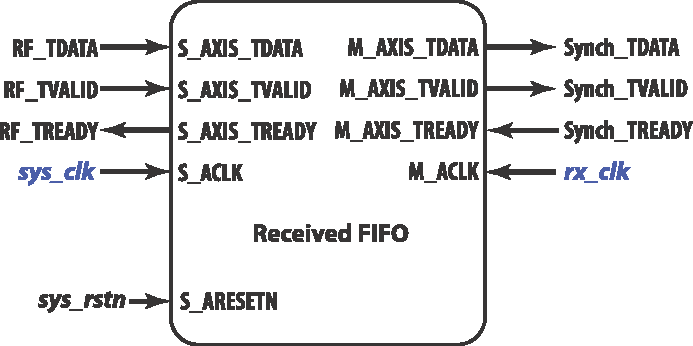
\includegraphics [width=0.5\columnwidth]{Figures/MSCR_RX_FIFO.pdf}
\caption{The receiver FIFO module.}
\label{fig:FIFO}
\end{figure}

\subsubsection{Synchronisation (Synch)}
Our CR system communicates in burst mode.
Hence, is must detect the presence of a frame and estimate the frequency offset required, based upon the preamble of the received frame.
The \emph{Synch} module performs estimation as discussed in Chapter~\ref{chap:Synchronisation}.
Fig.~\ref{fig:Sync} shows a block diagram of its implementation.

The timing metrics are calculated by using auto-correlation on received samples.
\emph{Coarse Time} detects the new frame and roughly estimates the start of a frame using blind estimation that provides generality for application to multiple standards.
By parameterising the length of $L$, the synchronisation module can effectively perform for three current supported standards as well as being extensible for future standards.

This module is implemented as a parameterised version with parameter $L$ whose values are defined together with the length of FFT ($N$), shown in Table~\ref{Tab:L}.
Combinations of $L$, and $N$ allow it to support multiple standards.
The parameterised values consist not only of the required combinations for 802.11, 802.16, and 802.22, but also support other combinations for future standards.
\begin{table}[h]
\centering
\caption{Parameterised values according to supported standards}{
\begin{tabular}{|l||*{6}{c|}}\hline
\theadset\theadfont\backslashbox[3em]{N}{L}
&\makebox[2.3em]{\thead{16}}&\makebox[2.3em]{\thead{32}}&\makebox[2.3em]{\thead{64}} &\makebox[2.3em]{128}&\makebox[2.3em]{\thead{256}}&\makebox[2.3em]{\thead{512}}\\\hline\hline
64 		& 802.11 & & & & & \\\hline
128 	& & & & & & \\\hline
256 	& & & 802.16 & & & \\\hline
512 	& & & & & & \\\hline
1024 	& & & & & & \\\hline
2048 	& & & & & & 802.22\\\hline
\end{tabular}
\label{Tab:L}
}
\end{table}

\begin{figure}
\centering
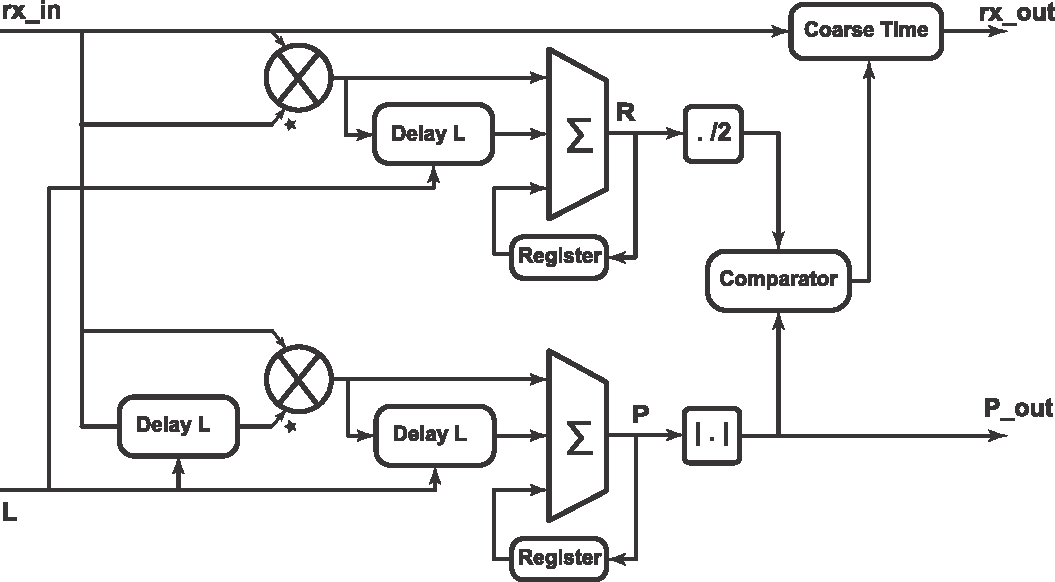
\includegraphics [width=0.8\columnwidth]{Figures/MSCR_RX_Sync.pdf}
\caption{Block diagram of Synchronisation module.}
\label{fig:Sync}
\end{figure}

\subsubsection{Frequency Compensation}
The \emph{FreComp} module performs fractional CFO estimation based on the value of $P$ passed from the previous module \emph{Synch}, as described in Chapter~\ref{chap:Synchronisation}.
Fractional CFO estimation and compensation are mathematically expressed as:
\begin{eqnarray}
\label{fractionalCFO}
\widehat{\Delta f } &=& \frac{\angle P}{2\pi \frac{L}{N}} \nonumber \\
\widehat{r[d]} &=& r[d] e^{-j2\pi\widehat{\Delta f} \frac{d}{N}}
\end{eqnarray}
where $\widehat{\Delta f }$ is estimated fractional CFO, $\angle P$ denotes the angle of P.
Fig.~\ref{fig:FFO} illustrates the process for frequency compensation.
A phase rotation sub-module is used to compensate fractional CFO by rotating the received sample phase by the correct angle.
This is calculated and accumulated based on estimated fractional CFO.
\begin{eqnarray}
\label{AccumCFO}
\phi[d] &=& \phi[d-1] + \frac{\angle P}{L} \nonumber \\
\widehat{r[d]} &=& r[d] e^{-j \phi[d]}
\end{eqnarray}

According to (\ref{AccumCFO}), the computation of \emph{FreComp} depends on the periodic length of short preamble that is used to calculate $P$.
Assuming that $L$ is normally defined as a power of two value, the division by $L$ can be effectively computed by a right shift.
Therefore, this module can be effectively implemented to support multiple standards by parameterising a right shifter according to the value of $L$.
\begin{figure}
\centering
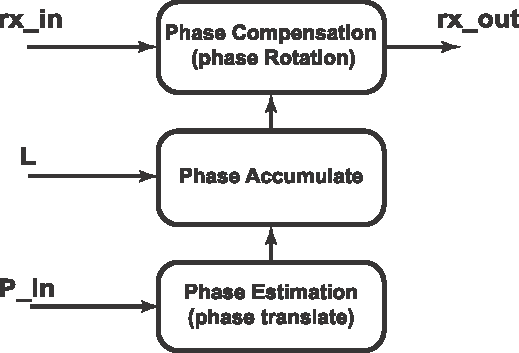
\includegraphics [width=0.4\columnwidth]{Figures/MSCR_RX_FFO.pdf}
\caption{Block diagram of frequency compensation module.}
\label{fig:FFO}
\end{figure}

\subsubsection{Fine STO Estimation}
\emph{FineSTO\_Est} estimates the starting sample of each OFDM symbol.
The RF front-end for MSCR need to access a wide range of frequencies, shown in Table~\ref{Tab:spec}. Depending on the standard being used, the CFO may be large, resulting in the presence of IFO.
Therefore, the implementation of \emph{FineSTO\_Est} is based on the algorithm presented in Chapter~\ref{chap:CFO} that is also robust to IFO.
The metric for fine STO estimation is expressed as:
\begin{equation}
\label{ProposedR}
S[d] =\sum_{m =0}^{L-1}   |r[d+m+L]|^2  |a[m]|^2,
\end{equation}
when $|a[m]|$ denotes the normalised amplitude of the preamble at the transmitter.

Fig.~\ref{fig:STO} shows the block diagram of fine STO estimation.
The metric is calculated based on a multiplierless correlation between received samples and transmitted preamble.
\emph{Peak Detect} finds the maximum value of correlation that is employed to accurately estimate the STO and \emph{Fine Time} determines the exact first sample of the next OFDM symbol (long preamble symbol).
However, multiplierless correlation is not flexible and the implementation depends on the preamble which is different for each standard.
Therefore, we employ PR module for the {FineSTO\_Est} module to obtain flexibility.
Each supported standard is implemented separately to a bitstream to be reconfigured at runtime by the \emph{CR engine} when the underlying standard is switched.
The PR region must be large enough to house the largest bitstream among the supported standards.
\begin{figure}
\centering
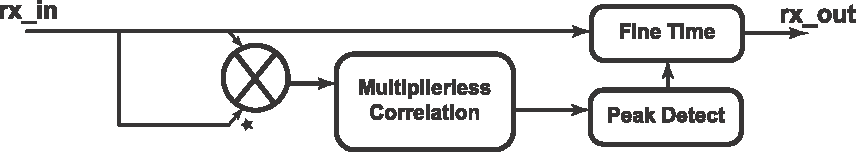
\includegraphics [width=0.6\columnwidth]{Figures/MSCR_RX_STO.pdf}
\caption{Block diagram of fine STO estimation module.}
\label{fig:STO}
\end{figure}

\subsubsection{Remove Cyclic Prefix}
\emph{RemoveCP} removes the cyclic prefix attached to each OFDM symbol.
The performance of this module depends on the length of CP $L_{CP}$ specified differently in each standards.
\emph{RemoveCP} consists of a counter to count from the beginning of each symbol and remove the CP samples if the counted value is smaller than $L_{CP}$
This module can be parameterised by adjusting $L_{CP}$ to support multiple standards.

\subsubsection{FFT}
\emph{FFT} is based on the Xilinx FFT/IFFT IP core, which supports modification of the FFT length at runtime to support different standards. When the standard is changed, the length of the FFT is modified using the relevant input. This reconfiguration completes within a few clock cycles.

\subsubsection{IFO Estimation and Channel Equalisation}
\emph{IFO\_Est\&Ch\_EstEqu} corrects IFO and performs channel equalisation.
IFO results in a cyclic shift in the frequency domain.
IFO is determined based on the method in Chapter~\ref{chap:CFO}:

\begin{equation}
\label{integerCFO}
\hat{\epsilon} =\underset{\tilde{\epsilon}}{\operatorname{argmax}}  \left|\sum_{k=0}^{N-1} Y^{*}[k-1] Y[k]  X^{*}[k-\tilde{\epsilon}]  X[k-1-\tilde{\epsilon}]\right|
\end{equation}
where $\epsilon$ denotes the value of IFO, $\hat{\epsilon}$, $\tilde{\epsilon}$ are estimated and trial values of $\epsilon$, respectively,
$Y(k)$ and $X(k)$ denote the $k^{th}$ frequency symbol index of the received subcarriers and the known transmitted preamble, respectively, and the OFDM symbol size $N$ is equal to the FFT size.

Fig.~\ref{fig:IFO} illustrates the block diagram of IFO estimation and channel equalisation.
\emph{IFO Correction} is performed effectively by cyclically shifting OFDM symbol corresponding to the estimated IFO estimation.

After compensating for IFO, the effects of the channel and residual STO must be taken into account to compensate the received sub-carriers.
Using information of the second preamble symbol, the effect of the channel can be estimated.
The estimation and compensation of channel and residual effects can be expressed as:
\begin{eqnarray}
\label{ChEqu}
Y[k] &=& X[k] * H[k] + N[k] \nonumber \\
H[k] &=& \frac{Y[k]-N[k]}{X[k]} \nonumber \\
\hat{H}[k] &=& \frac{Y[k]}{X[k]}\\
\label{ChCom}
\hat{R}[k] &=& \frac{R[k]}{\hat{H[k]}}
\end{eqnarray}
where $X[k]$, $Y[k]$ are the transmitted and received carriers in the preamble, respectively.
$H[n]$ represents for the channel and residual STO effect and $N[k]$ is the AWGN.
The equalization taps are estimated in (\ref{ChEqu}), and the compensation for received data carriers is given in (\ref{ChCom})
in which $R[k]$, $\hat{R}[k]$ denote received and compensated data carriers, respectively.

Since we use QPSK sub-carrier modulation, amplitude is not a concern. So, the complex division of channel estimation and compensation can be equivalently performed by multiplying by the conjugation of $X[k]$ and $\hat{H[k]}$, respectively.

This module depends on the second preamble that is specified differently for each standard.
Therefore, PR is used for the \emph{IFO\_Est\&Ch\_EstEqu} module to obtain effective standard-specific implementations.
\begin{figure}
\centering
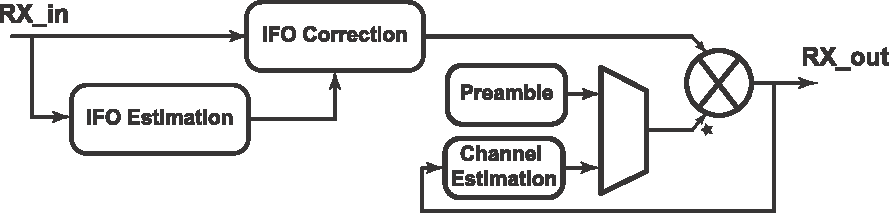
\includegraphics [width=0.7\columnwidth]{Figures/MSCR_RX_IFOCh.pdf}
\caption{The block diagram of IFO estimation and channel equalisation}
\label{fig:IFO}
\end{figure}

\subsubsection{Phase Tracking}
\emph{PhaseTrack} estimates the residual common phase error in each OFDM symbol after channel equalisation.
The \emph{PhaseTrack} implementation is based on an algorithm presented by Troya et al. \cite{Troya2007}.
The estimation is computed on the pilot symbols inserted in the OFDM symbol. The transmitted pilots are typically assigned
the values $\pm 1$. The residual phase error causes a phase rotation on received pilots.
\begin{eqnarray}
\label{PhaseTrack}
P_{k,l} = cos\theta_{l} -\alpha.k.sin \theta_{l} + j (sin\theta_{l} -\alpha.k.cos\theta_{l}),
\end{eqnarray}
where $P_{k,l}$ denotes the phase of received pilot which has frequency index $k$ in the $l^{th}$ OFDM symbol.
$cos\theta_{l} + j sin\theta_{l}$ is the residual common phase error of the $l^{th}$ OFDM symbol, and $\alpha$ is the slope of the phase distortion.
The residual common phase error is generally estimated for the supported standards as below:
\begin{eqnarray}
\label{CPE}
cos\theta_{l} &=& \frac{1}{N_P} \sum_{k \in S_P} \Re\{P_{k,l}\}, \\ \nonumber
sin\theta_{l} &=& \frac{1}{N_P} \sum_{k \in S_P} \Im\{P_{k,l}\}, \\ \nonumber
\end{eqnarray}
where $N_P$ denotes the number of received pilots employed for estimation, $S_P$ is a set of used pilot frequency indices.
The Fig.~\ref{fig:Phase} shows the block diagram of PhaseTrack. \emph{Pilot Extract} finds the employed pilots for phase tracking in the OFDM symbol based on allocation vector ($Alloc.~Bits$).
\emph{Phase Accumulator} computes the residual common phase error according to (\ref{CPE}).
The phase error is compensated for by multiplying the data carriers by the complex conjugate of the estimated common phase error.
To support multiple standards, $N_P$ is parameterised and $S_P$ can be determined through the allocation vector with the value shown in Table~\ref{tab:alloc_vec}

\begin{table}[h]
\centering
\caption{Allocation vector coding.}{
\label{tab:alloc_vec}
\renewcommand{\arraystretch}{1.3}
\begin{tabular}{@{}ll@{}}
\toprule
Subcarrier Type		&  Allocation Bits 	\\ \midrule
Null					&  00				\\
Data				&  10				\\
Positive pilot			&  01				\\
Negative pilot		&  11				\\
\end{tabular}
}
\end{table}
\begin{figure}
\centering
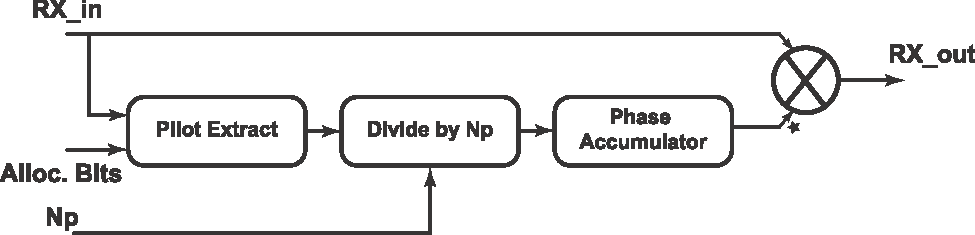
\includegraphics [width=0.7\columnwidth]{Figures/MSCR_RX_Phase.pdf}
\caption{Block diagram of phase tracking module.}
\label{fig:Phase}
\end{figure}

\subsubsection{Data symbol demodulation (\emph{DatSymDem})}
In the final step, the received bits are extracted from the data symbol by a data symbol demodulation block named \emph{DatSymDem}.
In the present implementation, this only supports QPSK modulation, but can be extended to support different data symbol modulations such as 16-QAM or 64-QAM in future, using the same basic interface.
All data symbols go through this module, and 2 bits are assigned to the output according to the sign bits of the real and imaginary parts of data symbol.


%---------------------------------------------------------------------------------
\section{Performance Analysis and Discussion}
\label{sec:PerAna}
%---------------------------------------------------------------------------------
\subsection{Latency and Stalling for PR-Based Baseband}

%\begin{figure*}[!t]
\begin{figure}
\centering{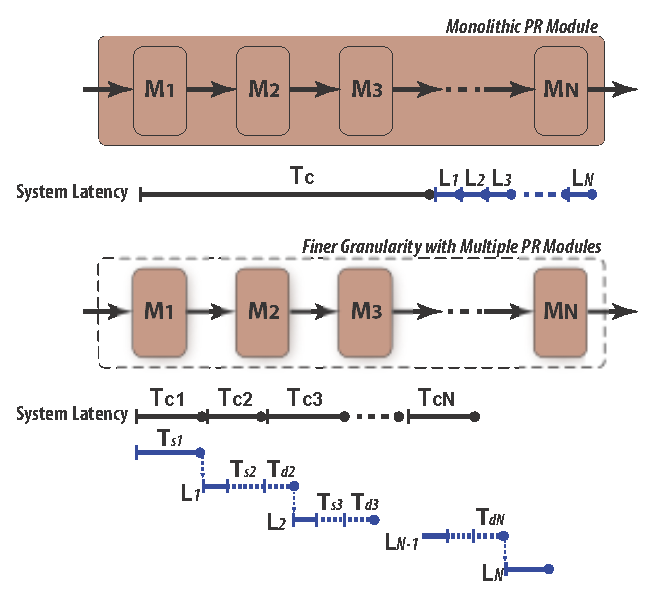
\includegraphics[width=1\columnwidth]{Figures/CRTiming.eps}}
\caption{Comparison of reconfiguration latency for a single and multiple PR modules.}
\label{fig:timing}
\end{figure}

One crucial challenge when implementing CR systems on reconfigurable hardware is long reconfiguration time when modifying the baseband.
PR can take a significant amount of time, especially for a large monolithic module.
In the case of the CR receiver, the system would have to stall during reconfiguration, potentially causing the loss of data packets and possibly even the loss of synchronisation.
A large FIFO would be required to store a stream of received samples long enough to overcome the reconfiguration latency when a large PR module is reconfigured.
A longer reconfiguration time would demand a larger FIFO, resulting in significantly increased hardware resource and power consumption.

We evaluate baseband latency for a monolithic PR module, as well as for a system employing a finer granularity with multiple PR modules, and a mix of PR and parameterised modules for the case when the system switches to a new baseband.
Fig.~\ref{fig:timing} illustrates this latency. We consider a system consisting of $N$ modules. $T_{c}$ refers to the reconfiguration time.
We assume that a module can not process data during its reconfiguration time.
$L_{i}$ is the computation latency of the $i^{th}$ module. Received data can, of course, be processed during the computation latency. In the case of a large monolithic PR module employed for the system, the system reconfiguration latency, $L_{sys}$, and halting time, $T_{hlt}$ that would require a FIFO to buffer received data which would otherwise be lost, is calculated as follow:

\begin{eqnarray}
\label{Mono}
L_{sys} &=& T_{c} + \sum_{i = 1}^{N}    (L_{i}) \nonumber \\
T_{hlt} &=& T_{c},
\end{eqnarray}

Finer granularity is possible by dividing the system into multiple sub-modules, each of which is implemented in a separate PR region. When a module is completely configured, it can process the received data while the following module is configured. Therefore, the system reconfiguration latency and halting time for the case of multiple PR modules can be calculated as follow;

\begin{eqnarray}
\label{Gran}
L_{sys} &=&  \sum_{i = 1}^{N} (T_{ci}) + T_{dN} + L_{N} \nonumber \\
T_{hlt} &=&  \sum_{i = 1}^{N}  (T_{si}),
\end{eqnarray}
where $T_{di}$ refers to the processing delay of the following module and $T_{si}$ is the stalling time to wait for configuration of the following module. If the computation latency of a module, $L_{i}$, is greater than the reconfiguration time of the following module,  $T_{ci+1}$, the following module has to delay operation by a duration $T_{di}$ before it receives input data for processing. Otherwise, the previous module is halted a duration $T_{si}$ until the following module is completely configured. The following module begins processing data just after its configuration is done ($T_{di} = 0$).

\begin{equation}
\label{DelayTime}
T_{di} = \begin{cases} Max(T_{ci}, T_{di-1}+L_{i-1}) - T_{ci}  	& i = 2..N, \\
						0 										& i = 1 \end{cases}  \\
\end{equation}
\begin{equation}
\label{HaltTime}
T_{si} = \begin{cases} T_{ci} - min(T_{ci}, T_{di-1}+L_{i-1}), 	&  i = 2..N, \\
					  T_{c1}									&  i=1 \end{cases}  \\
\end{equation}

Substituting the above equations into (\ref{Gran}),
\begin{eqnarray}
\label{Gran2}
L_{sys} &= & \sum_{i = 1}^{N}(T_{ci}) + L_{N} +   \nonumber \\
		& & (Max(T_{cN}, (Max( ... ) - T_{cN-1}) + L_{N-1}) - T_{cN})  \nonumber \\
T_{hlt} &= &\sum_{i = 1}^{N}(T_{ci})  -  \sum_{i = 2}^{N}  (min(T_{ci}, T_{di-1}+L_{i-1})),
\end{eqnarray}

We can see that system reconfiguration latency and halting time in the case of multiple PR modules is theoretically reduced thanks to being able to overlap the reconfiguration and data processing periods. Practically, the reconfiguration times are usually significantly greater than the processing latencies. This leads to $T_{di} = 0$ and  $min(T_{ci}, T_{di-1}+L_{i-1}) = L_{i-1}$ resulting in the approximated equations for (\ref{Gran2}) as below:
\begin{eqnarray}
\label{Gran3}
L_{sys} &= & \sum_{i = 1}^{N}(T_{ci}) + L_{N}    \nonumber \\
T_{hlt} &=  &\sum_{i = 1}^{N}(T_{ci})  -  \sum_{i = 1}^{N-1}  (L_{i}),
\end{eqnarray}

In addition, because of the optimisation in hardware compilation, the overhead of partitioning into multiple PR modules leads to the fact that $\sum_{i = 1}^{N}(T_{ci})$ is clearly greater than $T_{c}$, in (\ref{Mono}). Therefore, system reconfiguration latency, $L_{sys}$, and halting time, $T_{hlt}$ in (\ref{Gran2}) may be greater than that in (\ref{Mono}).
Generally, the finer granularity approach is only efficient in terms of system reconfiguration latency and halting time if the gain of overlapping the reconfiguration and data processing is greater than the overhead of partitioning into multiple PR modules.

Through the above analysis and comparison, we propose a new method employing a mix of PR modules and parameterised modules to obtain a significant reduction in system reconfiguration latency and halting time. For each module in the processing chain, commonalities across different operation modes are analysed. For modules requiring only minor modifications, parameterised versions are created.
For the $i^{th}$ module to be parameterised, the configuration time of this module can be eliminated because the parameterised modules can switch operating mode within one clock period. This approximately results in the following simplified equations;
\begin{eqnarray}
\label{Pro}
T_{ci} &\approx & 0   \nonumber \\
T_{si} &\approx & 0 \nonumber \\
T_{di} &\approx & T_{di-1} +  L_{i-1},
\end{eqnarray}

The above equations show the increasing efficiency of overlapping reconfiguration and data processing leading to a significant reduction in the system reconfiguration latency and halting time.

\subsection{Analysing the Proposed OFDM MSCR Approach}
We analyse the results of applying this method to the full receiver baseband  implemented on a xilinc Virtex~6 FPGA (XC6VLX240T).
We compare a large monolithic PR module, finer granularity PR, and the proposed mixture of PR and parameterisation.
To compute the configuration time of a PR module, we generate bitstreams for all modes.
The area of a PR region must satisfy the needs of the largest implementation it will house.
For the monolithic PR module, it is required that the PR module be able to contain the 802.22 OFDM baseband implementation, which is the largest receiver implementation among the three target implementations.

Similarly for the fine-grained approach, the configurations of the PR modules are computed based on the sub-modules of the 802.22 OFDM-based  implementation.
Table~\ref{tab:Resouces} reports the hardware resource usage for each sub-module and transmitter, receiver system for 802.22 on the Virtex~6 device. $M_1$, $M_2$, $M_3$, $M_4$, $M_5$, $M_6$, $M_7$, $M_8$ denote the functional modules of the OFDM based system: synchronisation, frequency compensation, fine STO estimation, remove CP, FFT, IFO estimation and channel equalisation, phase tracking, data symbol demodulation, respectively. $M_R$, $M_T$ are the monolithic receiver and transmitter sub-systems, respectively.
%Because we employ the multiplyless correlation for Fine STO estimation, DSP blocks are not used in this module but resulting in increased number of used slides.

We then determine the bitsteam size for each functional block according to the number of occupied CLB, DSP, BRAM columns that provide sufficient required resources for the block on FPGA floorplan. %\todo[inline]{How?} 
Fig.~\ref{fig:Bitstream} illustrates the bitstream sizes of each PR module, which we use to calculate configuration time later. The bitstream sizes of the sub-modules are relatively small compared to the monolithic PR module for the receiver sub-system. The $M_3$ bitstream is the largest among the sub-modules. The bitstream of the receiver is nearly triple the size of the transmitter.
\begin{table}[hb]
	\centering
	\caption{Resources for 802.22 OFDM-based implementation}
	\label{tab:Resouces}
	\begin{tabular}{l|c|c|c}
        \hline \hline
    			  \makebox[4.2cm][c]{$modules$}	&  \makebox[2cm][c]{Slices}  &   \makebox[2cm][c]{DSP} &   \makebox[2cm][c]{BRAM} \\
	\hline
		$M_1$(\textit{Synch})     				& 498 		& 5	& 0 \\
		$M_2$(\textit{FreComp})				& 474		& 4 	& 0 \\
		$M_3$(\textit{FineSTO\_Est})			& 2414	& 0 	& 0 \\
		$M_4$(\textit{RemoveCP})			& 23  		& 0	& 0 \\
		$M_5$(\textit{FFT})	  			& 1179  	& 15	& 11 \\
		$M_6$(\textit{IFO\_Est\&Ch\_EstEqu})	  	& 1249 	& 6	& 0 \\
		$M_7$(\textit{Phasetrack})	  		& 523  	& 3	& 0 \\
		$M_8$(\textit{DatSymDem})	  		& 4	  	& 0	& 0 \\
		$M_R$(Receiver)  					& 6363  	& 33	& 11 \\
		$M_T$(Transmitter)					& 1668  	& 15	& 11 \\
	\hline \hline
    \end{tabular}
\end{table}

\begin{figure}
\centering
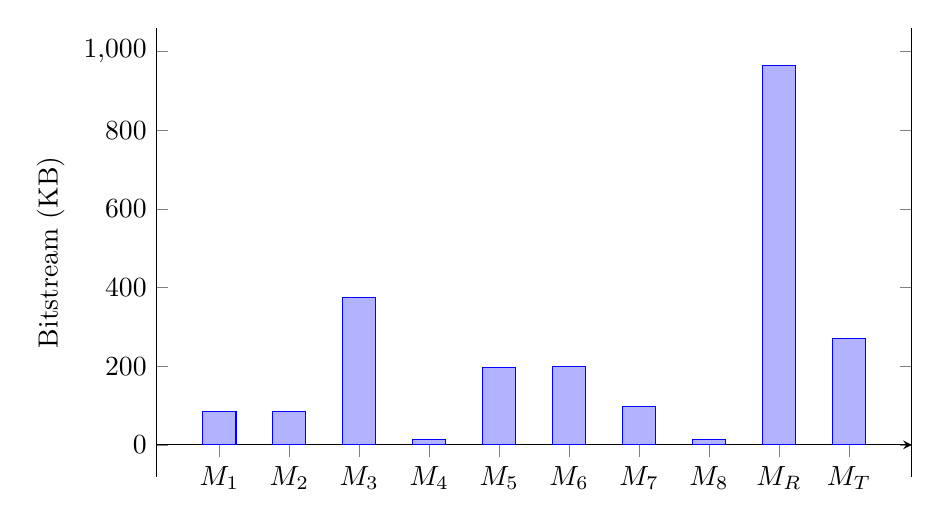
\begin{tikzpicture}[scale=1]
        \begin{axis}[
           axis x line=center,
           bar width=12pt,
           symbolic x coords={ $M_1$,$M_2$,$M_3$,$M_4$,$M_5$,$M_6$, $M_7$, $M_8$, $M_R$, $M_T$ },
           xtick=data,
	enlargelimits=true,
	ylabel={Bitstream (KB)},
	ylabel style={align=center},
%	xlabel={PR modules},
	ybar, x post scale=1.4]
            \addplot coordinates {
                ($M_1$,84.03) ($M_2$,84.03) ($M_3$,374.91) ($M_4$,14.54) ($M_5$,197.15) ($M_6$, 200.38)
                ($M_7$, 98.58) ($M_8$, 14.54) ($M_R$, 964.75) ($M_T$, 269.87)
               };
        \end{axis}
    \end{tikzpicture}
\caption{Bitstream sizes for PR modules.}
\label{fig:Bitstream}
\end{figure}

Processing latencies for functional modules are shown for the three standards in Fig.~\ref{fig:Latency}. We can see that 802.11 has the shortest latency because this standard uses the shortest FFT length, and hence the shortest symbol length for OFDM modulation.
It should be noted that during this latency the module still receives input data for processing.
The processing chain must be halted when the latency time has ended but the reconfiguration of the following module has not yet been completed. 
The worst case halting time is a case of the shortest latency and the longest reconfiguration time.
Therefore, the latencies for 802.11 are used to calculate system halting time.
%The latency of the synchronisation module depends on the timing offset that is the duration from the time between receiving input samples and the time when the first sample of the coming frame is received. The synchronisation module does not output data if no frame is detected. Generally, the synchronisation latency is calculated as $L_{1} = \mathit{Offset} + \mathit{processing time}$ \todo[inline]{Don't you have a symbol for processing time defined earlier??}.
%To evaluate the processing latency of the synchronisation module, the timing offset is considered to be equal to 0. We will consider the presence of timing offset later for calculating the system halting time and FIFO requirements.
\begin{figure}
\centering
\begin{tikzpicture}
        \begin{axis}[
           ylabel={Module Latencies (cycle)},
	ylabel style={align=center},
           xtick = data,
	axis x line=center,
           bar width= 6pt,
%	nodes near coords,
	legend style={at={(0.5, 1)}, anchor=south, legend columns=-1},
           symbolic x coords={$M_1$,$M_2$,$M_3$,$M_4$,$M_5$,$M_6$, $M_7$, $M_8$ },
	enlargelimits=true,
  	ybar, x post scale=1.4]
	\addplot[fill=F1] coordinates {
		($M_1$,137) ($M_2$,45) ($M_3$,84) ($M_4$,17) ($M_5$,216) ($M_6$, 153) ($M_7$, 66) ($M_8$,11)
           };
	\addplot[fill=F2] coordinates {
		($M_1$,153) ($M_2$,61) ($M_3$,100) ($M_4$,33) ($M_5$,616) ($M_6$, 553) ($M_7$, 252) ($M_8$,11)
           };
 	\addplot[fill=F3] coordinates {
		($M_1$,1048) ($M_2$,110) ($M_3$,1428) ($M_4$,513) ($M_5$,4226) ($M_6$, 4617) ($M_7$, 1273) ($M_8$,11)
            };
   	\legend{802.11, 802.16, 802.22}
        \end{axis}
\end{tikzpicture}
\caption{The latency of sub-modules for three standards}
\label{fig:Latency}
\end{figure}

Partial reconfiguration is performed with a high throughput ICAP controller that supports a data rate of 380\,MBps, closet to the theoretical limit of the FPGA.
%We also factor in the required sampling frequency for each chosen standard.
We use a sampling frequency of 10 MHz (i.e. the clock period = 0.1 us) that is typically defined for the 802.11p standard. %\todo[inline]{These sentences contradict!}
Compute latency is calculated for the 802.11 standard, as shown in Fig.~\ref{fig:CfgLat}.
%The values of latency are scaled by a factor of 10 for better observation.
As can be seen, the latency is very small in comparison to the configuration time.%\todo[inline]{Does that mean the graph is wrong? if the scales are different, use different axes!}
It is clear that overlapping reconfiguration and data processing is not sufficient to hide reconfiguration delay, and so the finer granularity approach may not improve significantly over the monolithic PR module.
\begin{figure}
\centering
\begin{tikzpicture}[scale=0.9]
%        \begin{axis}[
%           ylabel={Time (us)},
%	ylabel style={align=center},
%           xtick = data,
%	axis x line=center,
%           bar width= 9pt,
%%	nodes near coords,
%	legend style={at={(0.5, 1)}, anchor=south, legend columns=-1},
%           symbolic x coords={$M_1$,$M_2$,$M_3$,$M_4$,$M_5$,$M_6$, $M_7$, $M_8$ },
%	enlargelimits=true,
%  	ybar, x post scale=1.4]
%	\addplot[fill=F1] coordinates {
%		($M_1$,221.14) ($M_2$,221.14) ($M_3$, 986.61) ($M_4$, 38.27) ($M_5$, 518.82) ($M_6$, 527.33) ($M_7$, 259.41) ($M_8$,38.27)
%           };
%	\addplot[fill=F2] coordinates {
%		($M_1$,137) ($M_2$,45) ($M_3$, 84) ($M_4$, 17) ($M_5$, 21.6) ($M_6$, 153) ($M_7$, 33) ($M_8$, 01)
%           };
%	\legend{Configuration Time, Latency}
%        \end{axis}
 	\begin{axis}[
           ylabel={Configuration Time (us)},
	ylabel style={align=center, color=green},
 	ymin=0,
	width= 0.6*\textwidth,
           xtick = data,
	axis x line=center,
           bar width=10pt,
           symbolic x coords={0, $M_1$,$M_2$,$M_3$,$M_4$,$M_5$,$M_6$, $M_7$, $M_8$ },
	enlargelimits=0.15,
    	axis y line*=none,
  	ybar, x post scale=1.5]
	\addplot[fill=F1,shift={(-8pt,0)}] coordinates {
 		($M_1$,221.14) ($M_2$,221.14) ($M_3$, 986.61) ($M_4$, 38.27) ($M_5$, 518.82) ($M_6$, 527.33) ($M_7$, 259.41) ($M_8$,38.27) 
 		};
 	\end{axis}

	\begin{axis}[
           ylabel={Latency (us)},
	ylabel style={at={(1.05,0.5)}, color=blue},
 	ymin=0,
	width= 0.6*\textwidth,
           xtick = data,
	axis x line=center,
           bar width= 10pt,
	legend style={at={(0.5, 1.1)}, anchor=south, legend columns=2},
           symbolic x coords={0, $M_1$,$M_2$,$M_3$,$M_4$,$M_5$,$M_6$, $M_7$, $M_8$, 1},
	enlargelimits=0.15,
	axis y line*=right,
  	ybar, x post scale=1.5]
	\addplot [fill=F1] coordinates {($M_1$,0) ($M_2$,0) ($M_3$,0) ($M_4$, 0) ($M_5$, 0) ($M_6$, 0) ($M_7$, 0) ($M_8$, 0)};
	\addplot [fill=F2] coordinates {
 		($M_1$,13.7) ($M_2$,4.5) ($M_3$, 8.4) ($M_4$, 1.7) ($M_5$, 2.16) ($M_6$, 15.3) ($M_7$, 3.3) ($M_8$, 0.1)
		};
 	\legend{Configuration Time, Latency}
 	\end{axis}

\end{tikzpicture}
\caption{The configuration time and latency of sub-modules for OFDM-based MSCR system}
\label{fig:CfgLat}
\end{figure}

The system halting time is an accumulated value of the halting time in each module described in (\ref{HaltTime}). During the halting time, the processing chain is halted and a FIFO is required to buffer input samples. Because the halting time of the synchronisation module depends on the time when a new frame is detected. The timing offset must be taken into account. Given a scenario of a transmission, shown in Fig.~\ref{fig:tx-rx} when a standard switch is required, Both the transmitter and receiver spend time to reconfigure the system for the new baseband standard. In the proposed receiver, the synchronisation module is a parameterised module, so this module can change its function within a clock period and hence quickly process input samples. However, a new frame cannot be sent so quickly because the transmitter is still being reconfigured, resulting in a timing offset in the receiver. It is thus reasonable that the minimum timing offset can be chosen as the configuration time of the transmitter whose hardware characteristics were reported in Table~\ref{tab:Resouces}.
\begin{figure}
\centering
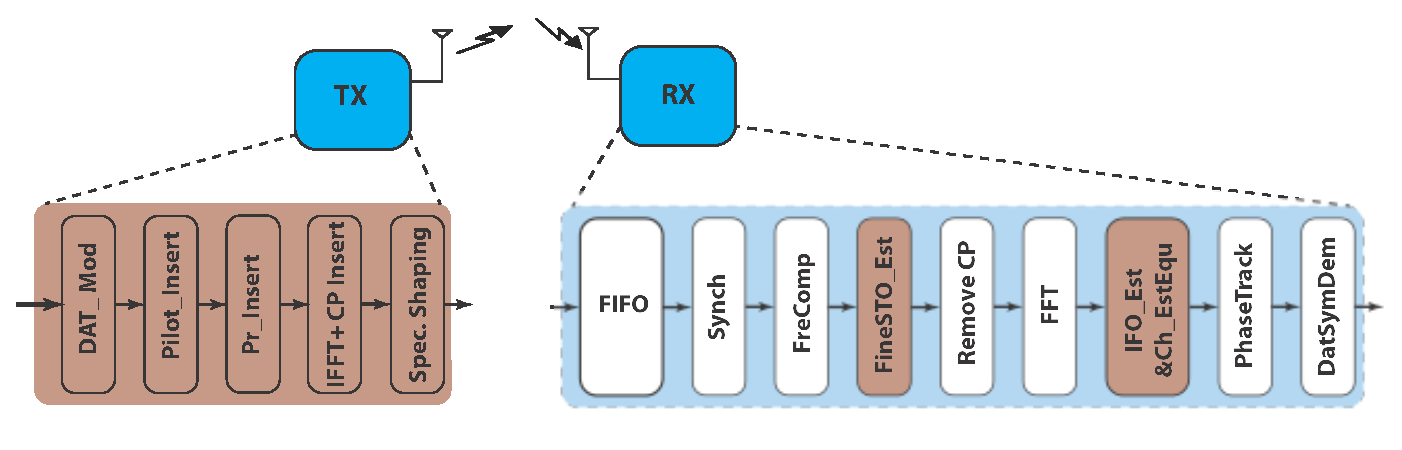
\includegraphics [width=1\columnwidth]{Figures/CR_Tx-Rx.eps}
\caption{A scenario of a transmission}
\label{fig:tx-rx}
\end{figure}

\definecolor{M1}{HTML}{FFFFd9}
\definecolor{M2}{HTML}{edF8b1}
\definecolor{M3}{HTML}{c7e9b4}
\definecolor{M4}{HTML}{7Fcdbb}
\definecolor{M5}{HTML}{41b6c4}
\definecolor{M6}{HTML}{1d91c0}
\definecolor{M7}{HTML}{225ea8}
\definecolor{M8}{HTML}{253494}
\definecolor{MR}{HTML}{081d58}
\begin{figure}
\centering
\begin{tikzpicture}
\begin{axis}[
	xbar stacked,
	legend style={at={(0.7, 1.1)}, anchor=south, legend columns=3},
    	ytick=data,
    	axis y line*=none,
    	axis x line*=bottom,
	tick label style={font=\footnotesize},
    	bar width= 20pt,
    	xlabel={Time (us)},
    	yticklabels={Mon, Mul , Pro},
    	xmin=0,
%    	xmax=600,
    	area legend,
    	y=12mm,
    	enlarge y limits={abs=0.625}, x post scale=1.4
	]
	\addplot [M1,fill=M1] coordinates {(0,0) (221.14,1) (0 ,2) };
	\addplot [M2,fill=M2] coordinates {(0,0) (214.28,1) (0,2) };
	\addplot [M3,fill=M3] coordinates {(0,0) (984.36,1) (258.22,2) };
	\addplot [M4,fill=M4] coordinates {(0,0) (034.07,1) (0,2) };
	\addplot [M5,fill=M5] coordinates {(0,0) (517.97,1) (0,2) };
	\addplot [M6,fill=M6] coordinates {(0,0) (516.53,1) (495.63,2) };
	\addplot [M7,fill=M7] coordinates {(0,0) (251.76,1) (0,2) };
	\addplot [M8,fill=M8] coordinates {(0,0) (034.97,1) (0,2) };
	\addplot [MR,fill=MR] coordinates {(2538.82,0) (0,1) (0,2)};
	\legend{$Ts_1$,$Ts_2$,$Ts_3$,$Ts_4$,$Ts_5$,$Ts_6$, $Ts_7$, $Ts_8$ , $Ts_R$}
\end{axis}
\end{tikzpicture}
\caption{ The halting time comparison of the system for three different approaches.}
\label{fig:Halt}
\end{figure}
%\todo[inline]{Fix the colours so they print ok in black and white.}

Fig.~\ref{fig:Halt} shows the system halting time of the three approaches. $Mon$, $Mul$, $Pro$ denote the halting time of the monolithic PR module approach, the multiple PR module approach, and the proposed approach, respectively. %\todo[inline]{Why not put them in the same order in the graph?}
$Ts_n$ is the halting time of the corresponding $M_n$ functional module. $Ts_R$ is the halting time of the monolithic receiver sub-system.

We can see that the halting time of the multiple PR module approach is greater than that of the monolithic PR module approach, because the gain achieved by overlapping reconfiguration and data processing is less than the overhead incurred by partitioning into multiple PR modules. The proposed approach can significantly reduce the halting time to less than one-third of that of the monolithic PR module approach. This results in a reduction in FIFO buffering requirements.
\begin{figure}
\centering
\begin{tikzpicture}[scale=0.9]
 	\begin{axis}[
           ylabel={System reconfiguration latency (us)},
	ylabel style={align=center, color=green},
 	ymin=0,
	width= 0.6*\textwidth,
           xtick = data,
	axis x line=center,
           bar width= 14pt,
           symbolic x coords={0, $Mon$, $Mul$, $Pro$},
	enlargelimits=0.2,
    	axis y line*=none,
  	ybar, x post scale=1.2]
	\addplot[fill=F1,shift={(-10pt,0)}] coordinates {($Mon$,4190.82) ($Mul$,2811.12) ($Pro$,753.97)  };
 	\end{axis}

	\begin{axis}[
           ylabel={FIFO requirement (KSs)},
	ylabel style={at={(1.1,0.5)}, color=blue},
 	ymin=0,
	width= 0.6*\textwidth,
           xtick = data,
	axis x line=center,
           bar width= 14pt,
	legend style={at={(0.5, 1.1)}, anchor=south, legend columns=2},
           symbolic x coords={0, $Mon$, $Mul$, $Pro$, 1},
	enlargelimits=0.2,
	axis y line*=right,
  	ybar, x post scale=1.2]
	\addplot [fill=F1] coordinates {($Mon$,0) ($Mul$,0) ($Pro$,0) };
	\addplot [fill=F2] coordinates {($Mon$,64) ($Mul$,64) ($Pro$,16)  };
 	\legend{Latency, FIFO}
 	\end{axis}

\end{tikzpicture}
\caption{A comparison of the three approaches in terms of system reconfiguration latency and FIFO requirements.}
\label{fig:LatFIFO}
\end{figure}

\begin{table}[hb]
	\centering
	\caption{Memory resources for 32 bit AXI4 interface FIFOs implementation}
	\label{tab:FIFOResouces}
	\begin{tabular}{c|c|c}
        \hline \hline
    			  \makebox[4.2cm][c]{FIFO size (KSs)}	&  \makebox[3cm][c]{18K BRAM}  &  \makebox[3cm][c] {36K BRAM} \\
	\hline
%		4     		& 0 	&  4 \\
		8			& 1	&  7 \\
		16			& 1	&  14  \\
		32			& 0 	&  29 \\
		64	  		& 0  & 58 \\
		128	  		& 0	 & 116 \\
	\hline \hline
    \end{tabular}
\end{table}
Fig.~\ref{fig:Halt} compares the three approaches in terms of system reconfiguration latency and FIFO buffering requirements. The system latencies are computed in the worst case which is the latency for the 802.22 standard. The FIFO requirements are calculated based on multiplying the sampling frequency by the halting time, followed by rounding up to the next power of two.  Table~\ref{tab:FIFOResouces} reports
required resources for 32 bit AXI4 interface FIFO implementation with some different availabe size configurations. 
%\todo[inline]{Why do you have to round up? FIFOs can be any length} 
The system reconfiguration latency of the proposed method is significantly reduced to 18~\% and 27~\% of the system reconfiguration latency of the monolithic PR module and the multiple PR module approaches, respectively. The FIFO requirement for the proposed approach is only 16 kilo-samples (KSs) while the other approaches require a FIFO to store up to 64~KSs.
%\todo[inline]{I thought we said we need actual FIFO implementation results?Also, I need to understand what this system latency number means.}

%---------------------------------------------------------------------------------
\section{Summary}
%---------------------------------------------------------------------------------
We have shown that configuring a radio baseband composed of multiple modules can be made more efficient in terms of time, and buffering requirements, by mixing parameterisation and PR.
Implement the whole baseband as a single PR module leads to long reconfiguration time, during which no processing can be performed, and hence significant FIFO buffering to prevent loss of samples in the receiver.
Breaking the baseband chain into multiple PR modules could be beneficial as it would allow individual modules to start processing as the complete their reconfiguration, overlapping this processing with the reconfiguration of the next module. However, since reconfiguration time is significantly higher than the computational latency, we find that the benefit is outweighed by the overhead of multiple PR modules.
Our proposed approach only applies PR to modules where different modes are very different in hardware, with other modules designed to be parameterisable. As a result, overall halting time is reduced by more than half.
The FIFO buffering requirement of the proposed method is also decreased to 25~\% of that required for the other methods.
We are working on finalising a demonstrator for this approach.
\chapter{A Novel Architecture for Multiple Standard Cognitive Radios}
\label{chap:MSCR}
%%!TEX root = main_thesis.tex
%---------------------------------------------------------------------------------
\chapter{Conclusions and Future Work}
\label{chap:conclusion}
%---------------------------------------------------------------------------------
This thesis has presented techniques for implementing robust, low-power cognitive radios using modern FPGAs. We have shown that the computational performance of FPGAs allows us to develop techniques for more advanced synchronisation, leading to robustness in fading channels, that we can control spectral leakage to satisfy even very strict constraints defined by recent standards, and that a multi-standard radio can be built to minimise reconfiguration time by mixing the use of partial reconfiguration and parameterised modules. The contributions made serve as important building blocks in developing a functional dynamically reconfigurable OFDM cognitive radio.

This chapter concludes the thesis, highlighting the contributions and suggesting ideas for future research.

\section{Summary of Contributions}

This thesis has worked towards the implementation of dynamically configurable cognitive radios on FPGAs.
With this goal in mind, we identified key challenges including robust synchronisation and shaping spectral leakage.
We proposed novel contributions in the field to address these challenges, in each case focusing on applicability in efficient hardware implementations.
We have also explored the system-level challenge of reconfiguration time in radios implemented with partial reconfiguration, and proposed a mixed parametrisation approach for minimising reconfiguration time.

\subsection{Robust, Efficient Synchronisation}

In Chapter~\ref{chap:BackgroundLiterature}, we presented the theory behind OFDM and demonstrated the importance of robust synchronisation, especially in complex channels like those in moving vehicles, or when building flexible radios with less tuned components.
We proposed a multiplierless correlation method for basic timing synchronisation in Chapter~\ref{chap:multiplierlesscorrelator} that can reduce power and area while maintaining performance close to full cross correlation.
We presented a more complex timing metric and its efficient implementation in Chapter~\ref{chap:Synchronisation}, showing robust CFO and STO synchronisation in frequency selective channels, and a computational complexity close to less robust standard methods.
In Chapter~\ref{chap:CFO} we presented a novel method for CFO estimation that tolerates larger CFO variations than existing methods, allowing for flexible radios to be built with support for wide ranging frequency bands without overly expensive RF components.
These methods together offer practical implementations that are more robust than any other published implementations.

\subsection{OFDM Spectrum Shaping}
We discussed in Chapter~\ref{chap:BackgroundLiterature} that OFDM suffers from large sidelobes due to the addition of subcarrier sync pulses.
In the context of cognitive radios opportunistically accessing radio spectrum, typically leads to a reduction in usable bandwidth as some subcarriers are switched off to reduce potential interference with adjacent channels.
In Chapter~\ref{chap:SpectralLeakage}, we presented a novel method incorporating filtering at the baseband that can offer much better sidelobe suppression, meeting even very stringent requirements in modern CR standards. We demonstrated this approach applied to 802.11p and 802.11af waveforms, and demonstrated its feasibility in hardware.
We also showed that the proposed architecture could flexibly adjust this shaping for moving bands in a CR setting.

\subsection{Multi-Standard Radio Design}

In Chapter~\ref{chap:MSCR}, We presented a detailed analysis of incorporating partial reconfiguration for adapting an FPGA-based CR.
We showed that while PR offered low resource utilisation, long reconfiguration time could be a concern. We showed that mixing PR modules with parametrised modules offered a significant reduction in reconfiguration time, allowing radios to be implemented with internal buffering to overcome data loss during reconfiguration.
We also showed how a clock frequency tuning technique could offer seamless recovery following reconfiguration.

\section{Future Research Directions}

Our achievements in this thesis have helped us identify crucial questions to be explored in future along this line. And while we have been able to test our designs in hardware, building a fully functional radio system is something that still requires some engineering design effort.

\subsection{Increasing Spectrum Efficiency with Shaping for NC-OFDM}
The shaping approach presented in Chapter~\ref{chap:SpectralLeakage} offers high out of band attenuation, avoiding interference with neighbouring channels, while allowing use of subcarriers close to adjacent channels.
It could also be applied to in-band shaping in the context of con-contiguous OFDM signals, where some intermediate subcarriers are switched off due to the presence of other uses in intermediate bands.
This could result in significant efficiency improvements in the case of highly fragmented bands, since narrow spaces can still be used effectively

\subsection{Efficiently Adaptive Shaping Spectral Leakage}
The static strict SEMs in radio systems can guarantee that the systems mitigate the effect of ICI. However, the implementation and power cost may be significant.
In practice, adjacent channels are not always occupied and the communication range can change from time to time. Therefore, statically maintaining a very strict SEMs may be wasteful in terms of computation.
One approach would be to dynamically modify the SEM based on occupancy of adjacent channels and current transmit power.
This would mean that in some cases the SEM would be relaxed compared to the static implementation, allowing improved computational efficiency and lower computational power.

\subsection{Standardised Software Interface for Multi-Standard Radio Platform}
We have discussed that there are a variety of different cognitive radio platforms, many of which do include some FPGA capability. However, this interface between higher layers and hardware baseband processing is often implemented in an ad-hoc manner. Our group is exploring how a standardised interface might be proposed to allow higher layer cognitive stacks to be coupled with different baseband systems, including both the data stream interface, and the control. This must entail minimal latency, and enable the strengths of the baseband in terms of high data stream throughput.

\subsection{Alternative MultiCarrier Modulations Techniques}
While OFDM is well established, other multicarrier schemes have been proposed which offer advantages. Demonstrating efficient mapping of these schemes to high performance baseband hardware is important for them to gain traction.
Generalised Frequency Division Multiplexing (GFDM) is a new modulation scheme that overcomes some of OFDM's limitations.
In GFDM, out of band spectrum is compressed by an adjustable pulse shaping filter for individual subcarriers. Transmission efficiency is increased thanks to a two-dimensional data process (grouping data symbols across subcarriers and time slots).
However, it suffers from higher bit error rates (because of the interference between subcarriers and time slots) and requires increased computational resources to implement the prototype filter.
A similar structure means a radio supporting both OFDM and GFDM could be developed, allowing experimentation with this new standard, while offering backwards compatibility.

\subsection{Higher Layer Knowledge to Minimise Reconfiguration Time}
As radios support more standards, switching between them can become time-consuming since many modules need to be reconfigured. One way of overcoming this is using knowledge about the most likely reconfiguration options to prepare the require partial bitstreams in advance, or even to drive the design decision to parameterise some modules that would otherwise use PR.
This information could be forthcoming from higher layers through collaborative decision making or modelling of the dynamic properties of the channel.

\section{Summary}

This thesis has presented key contributions to allow for the design of dynamically reconfigurable cognitive radios on FPGAs. FPGAs, especially recent devices like the Xilinx Zynq, offer an ideal platform for building radios with flexible baseband processing and high level software control. We are confident that these contributions will help make this vision a reality in the near future.

\chapter{Conclusion and Future Work}
\label{chap:conclusion}




% -------------------------------------------------------------------------------- %
% --------------------------- Part III. The Back Matters ------------------------- %
% -------------------------------------------------------------------------------- %
\appendix
%%---------------------------------------------------------------------------------
\chapter{Appendix}
\label{chap:Appendix}
%---------------------------------------------------------------------------------
\section{Kronecker Product}\label{appen:Kronecker}
The Kronecker product is also called matrix direct product and is
usually represented as $\otimes$. For example, the Kronecker product
a $2\times2$ matrix $A$ and a $3\times2$ matrix $B$ is define as
\begin{eqnarray}\label{Kronecker}
    A\otimes B &=& \left(%
\begin{array}{cc}
  a_{11}B & a_{12}B \\
  a_{21}B & a_{22}B \\
\end{array}%
\right)\nonumber\\
&=&\left(%
\begin{array}{cccc}
  a_{11}b_{11} & a_{11}b_{12} & a_{12}b_{11} & a_{12}b_{12} \\
  a_{11}b_{21} & a_{11}b_{22} & a_{12}b_{21} & a_{12}b_{22} \\
  a_{11}b_{31} & a_{11}b_{32} & a_{12}b_{31} & a_{12}b_{32} \\
  a_{21}b_{11} & a_{21}b_{12} & a_{22}b_{11} & a_{22}b_{12} \\
  a_{21}b_{21} & a_{21}b_{22} & a_{22}b_{21} & a_{22}b_{22} \\
  a_{21}b_{31} & a_{21}b_{31} & a_{22}b_{31} & a_{22}b_{32} \\
\end{array}%
\right)
\end{eqnarray}
The result is a $6\times4$ matrix, where any elements from the $A$
is multiplied with any elements from $B$. For general case, the
Kronecker product of a $M\times N$ matrix $A$ and a $P\times Q$
matrix $B$, the resulting matrix is $MP\times NQ$, and the elements
of the resulting matrix is defined as
\begin{equation}\label{Kronecker2}
    c_{\alpha,\beta}=a_{ij}b_{kl}
\end{equation}
where
\begin{eqnarray}
% \nonumber to remove numbering (before each equation)
  \alpha &=& P(i-1)+k \\
  \beta &=& Q(j-1)+l
\end{eqnarray}
      % Appendix and Publications
%\chapter* {Publication}
\addcontentsline{toc}{chapter}{\numberline{}\hspace{-0.24in}{\bf
Publication}}




% Include the references
\newpage
\addcontentsline{toc}{chapter}{References}
\bibliographystyle{ieeetr}      % Use the IEEE bibiography style
\bibliography{ConfirRpt_macro,ConfirRpt}  % Include the BibTex files





\end{document}      % End of the text



% ------------------
% End of the File
% ------------------
